%%____________________________________________________________________________||
\chapter{Transfer factors}
\label{app:nominal-tf}
The nominal values of the transfer factors from the control regions to the signal region are shown in Figures~\ref{fig:tfSyst_nominal_mu}
-\ref{fig:tfSyst_nominal_mumug}. Missing entries do not meet the requirement of statistical uncertainty from simulated
events of less than $50\%$.
\begin{figure}[!h]
  \centering
\subfloat[$\mj \rightarrow (\znunu)$]{
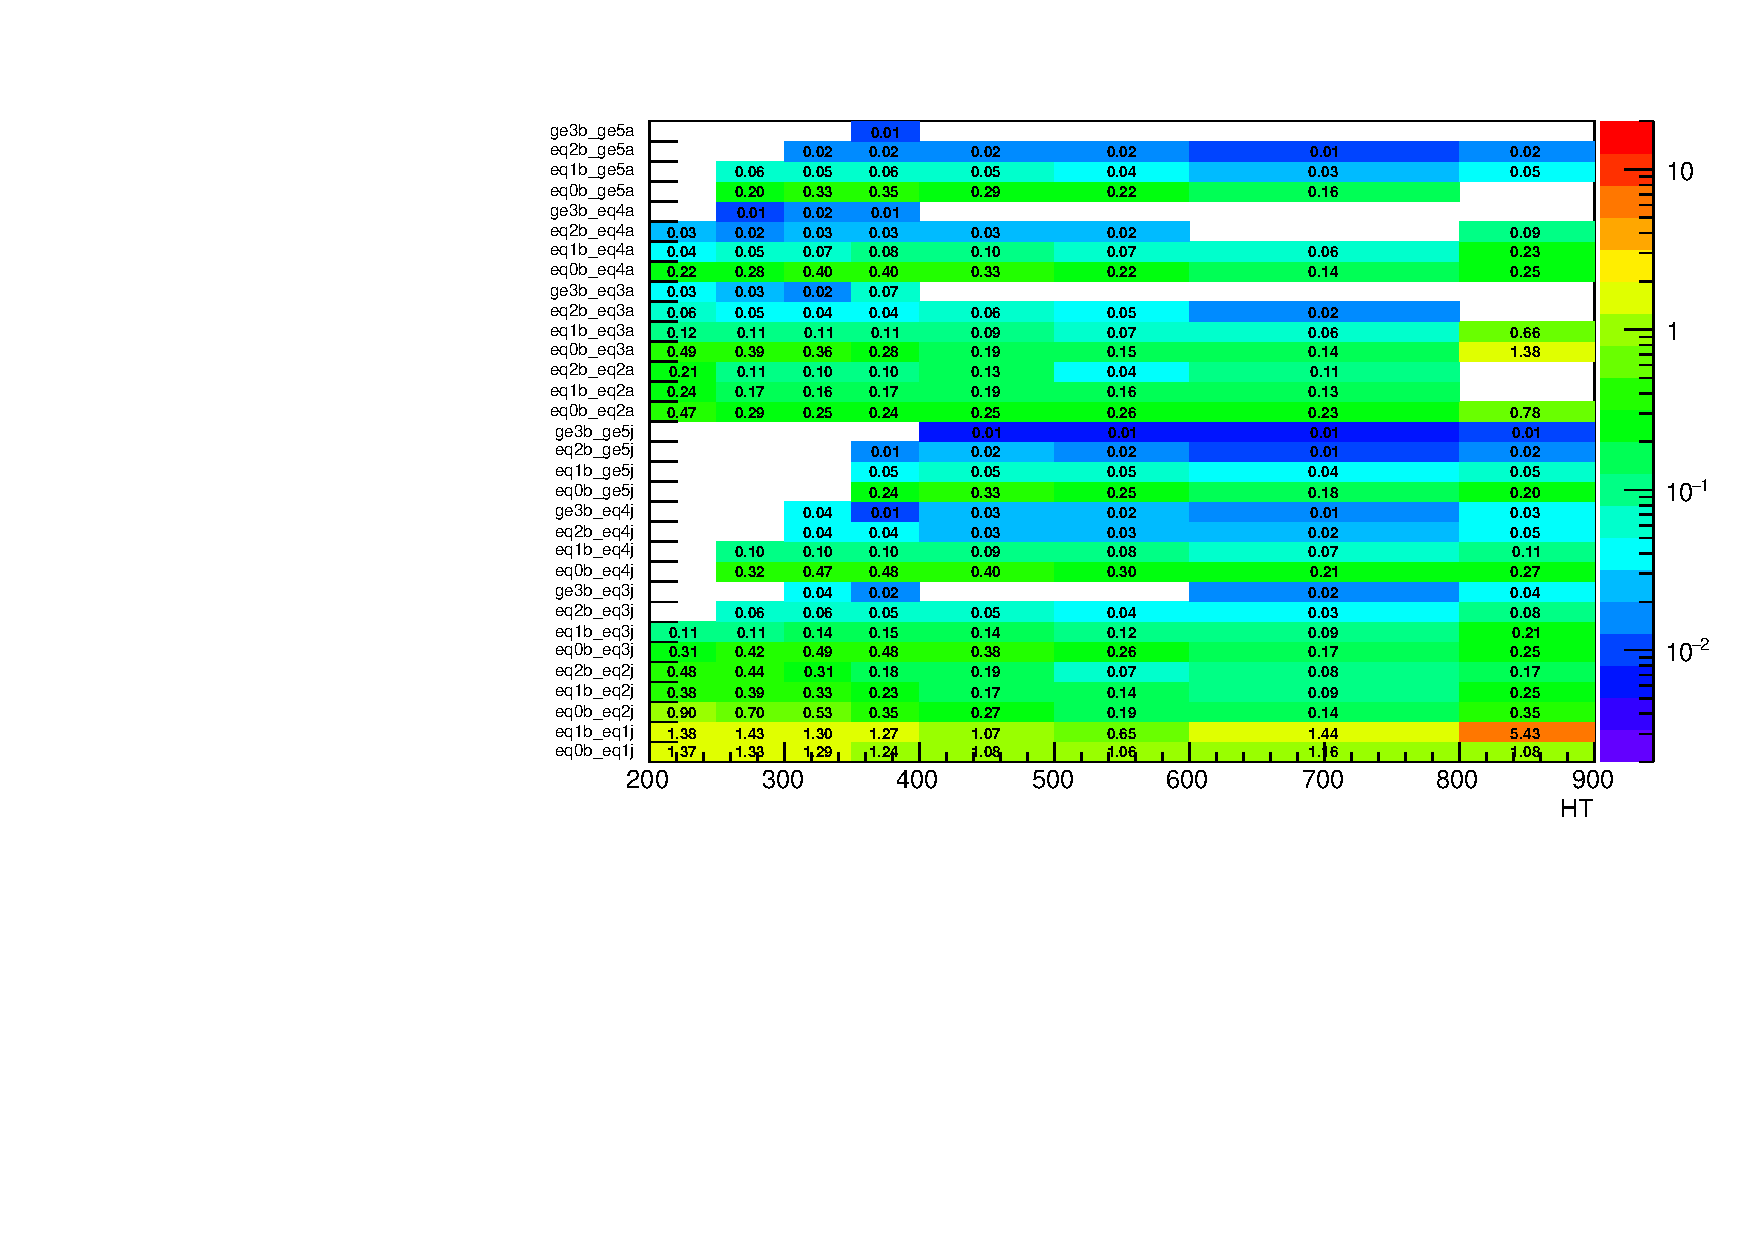
\includegraphics[width=0.49\textwidth]{Figures/backgroundPrediction/mcSystematics12p9fb/Zinv/mu/tfh_ht_mht_all.pdf}
  }~~
\subfloat[$\mj \rightarrow (\ttW)$]{
    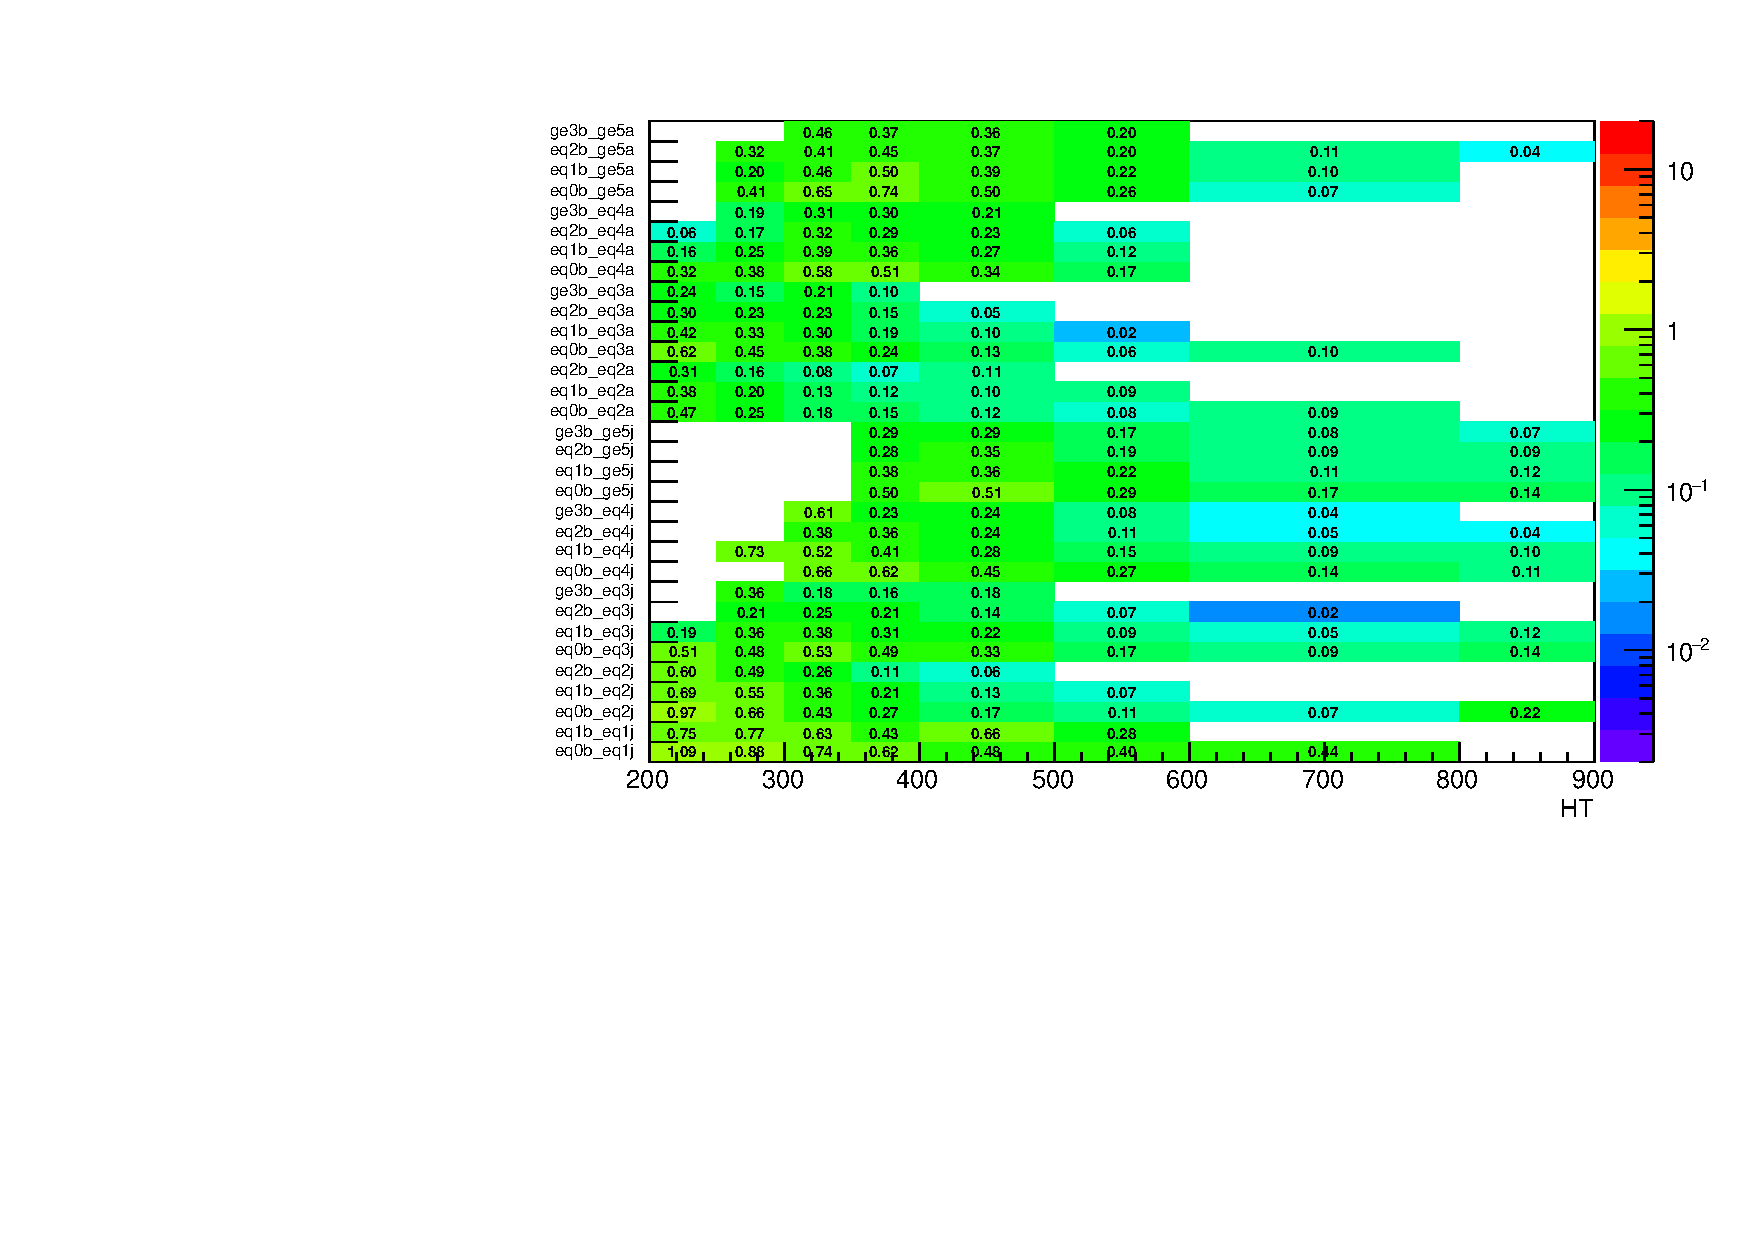
\includegraphics[width=0.49\textwidth]{Figures/backgroundPrediction/mcSystematics12p9fb/Ttw/mu/tfh_ht_mht_all.pdf}
  }
\caption{\label{fig:tfSyst_nominal_mu} The $\mj$ transfer factors as a function of \scalht and jet category.}
\end{figure}

\begin{figure}[!h]
  \centering
\subfloat[$\mmj \rightarrow (\znunu)$]{
    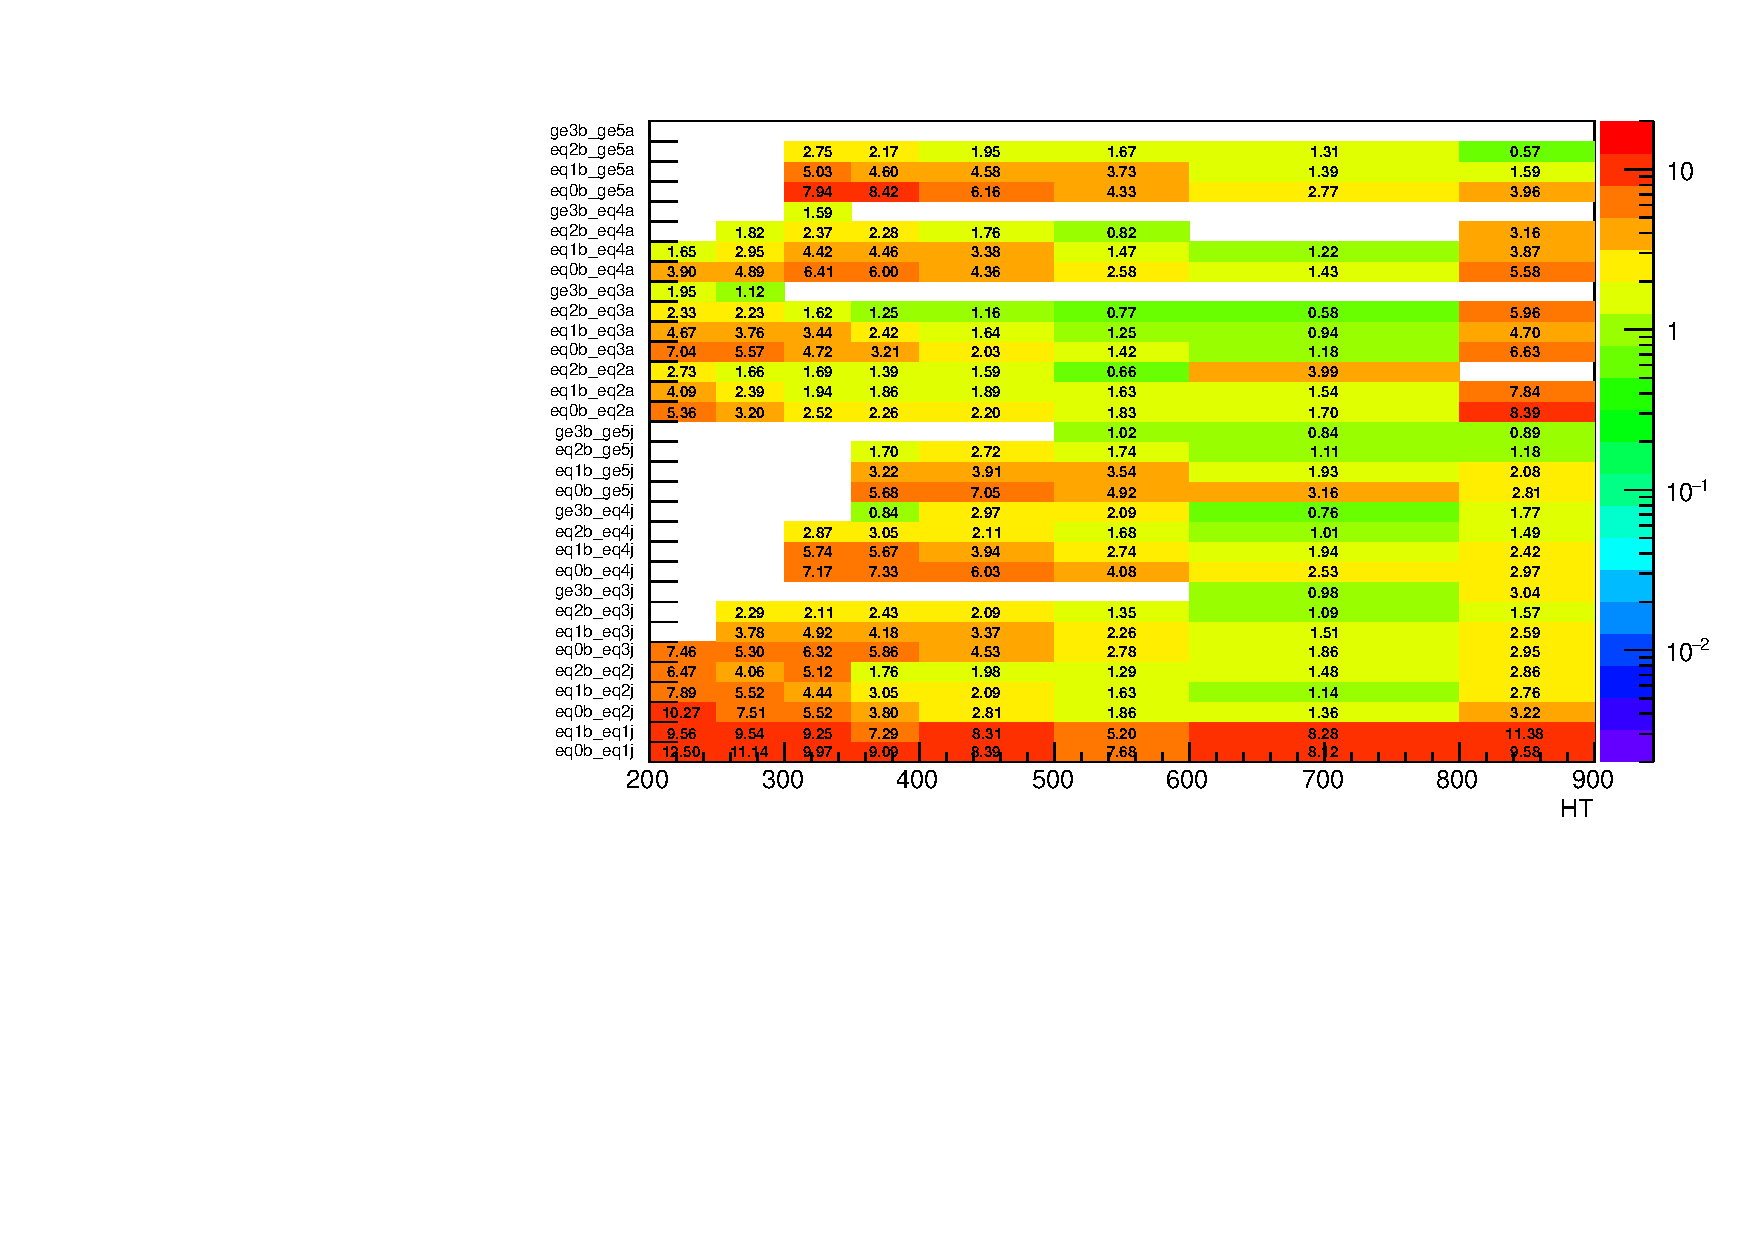
\includegraphics[width=0.49\textwidth]{Figures/backgroundPrediction/mcSystematics12p9fb/Zinv/mumu/tfh_ht_mht_all.pdf}
    }~~
\subfloat[$\gj \rightarrow (\znunu)$]{
    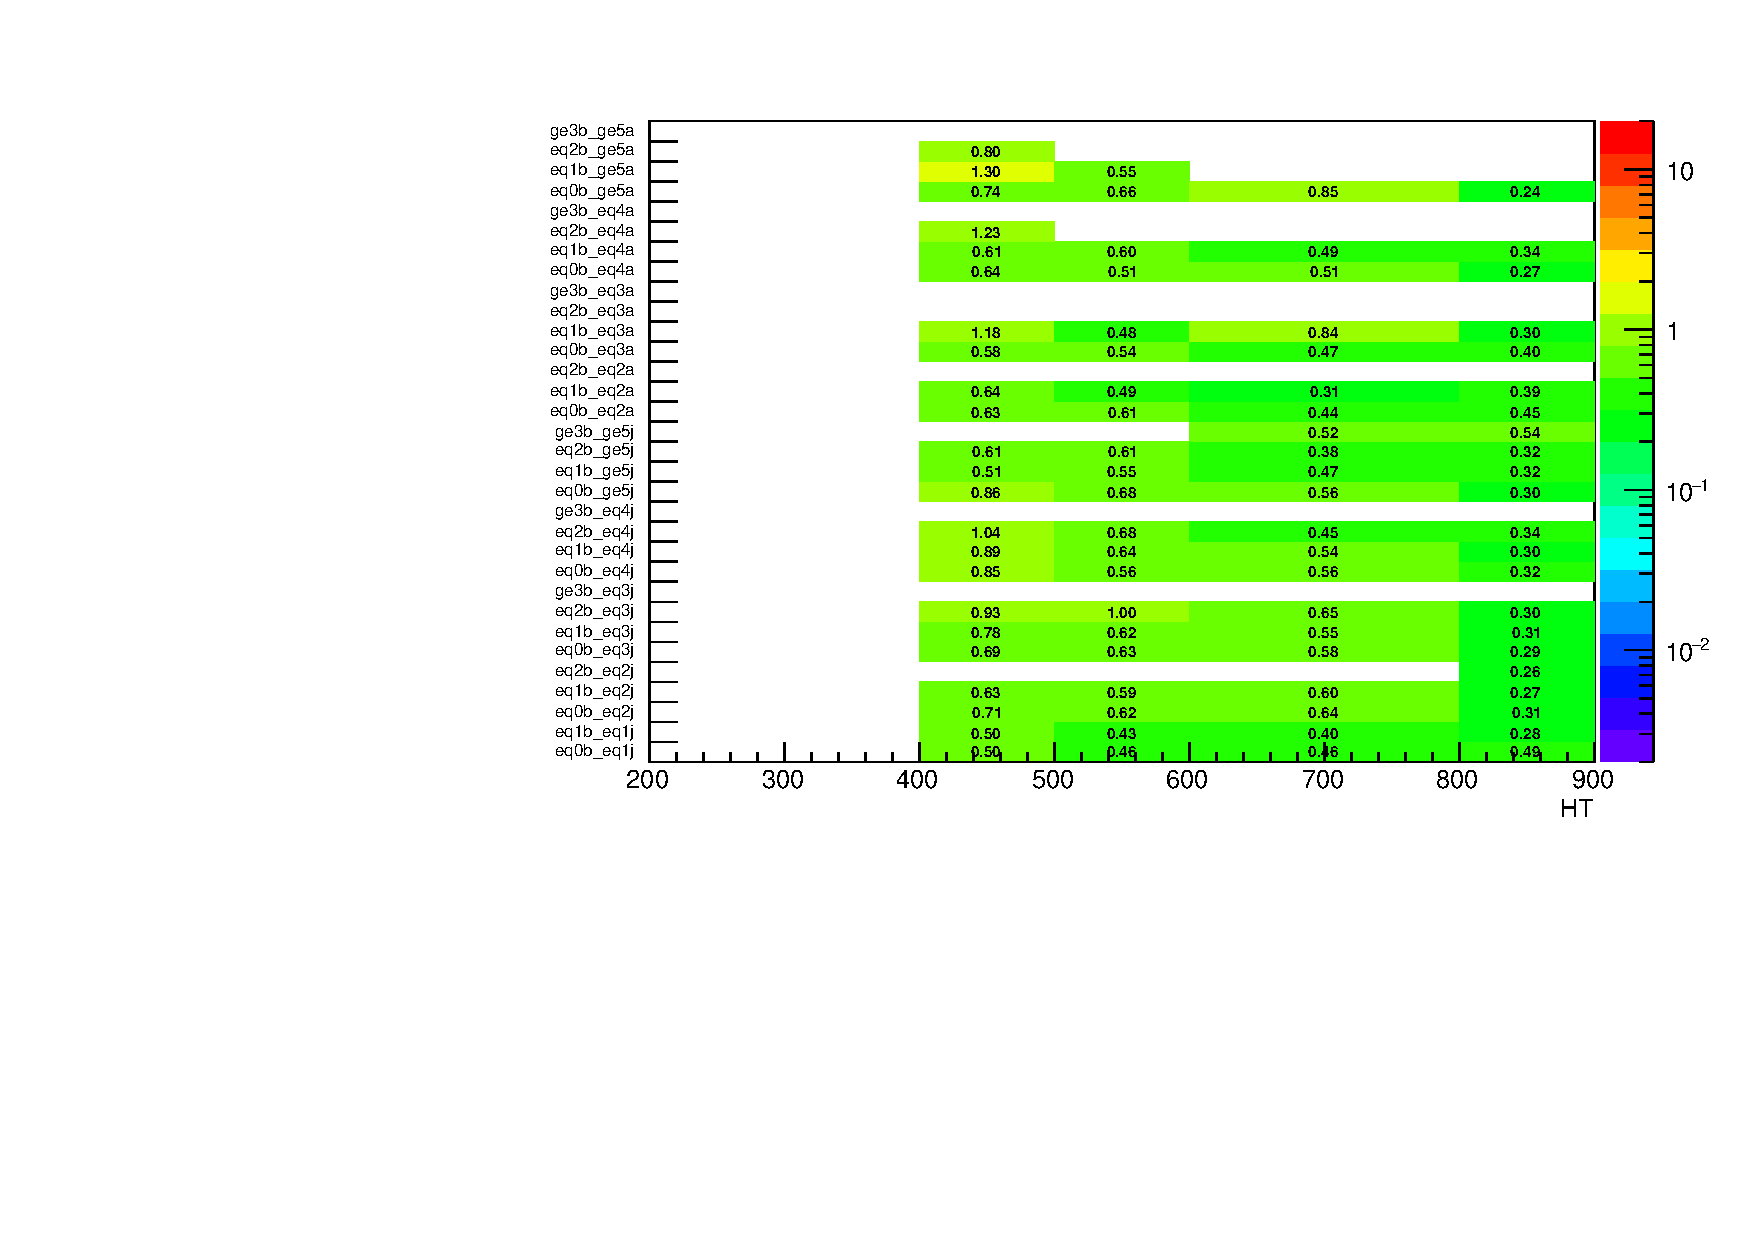
\includegraphics[width=0.49\textwidth]{Figures/backgroundPrediction/mcSystematics12p9fb/Zinv/gj/tfh_ht_mht_all.pdf}
    }
\caption{\label{fig:tfSyst_nominal_mumug} The $\mmj$ and $\gj$ transfer factors as a function of \scalht and jet category.}
\end{figure}


% \section{Jet energy scale}
% \begin{figure}[!h]
%   \centering
%   \subfloat[JEC up variation]{
%     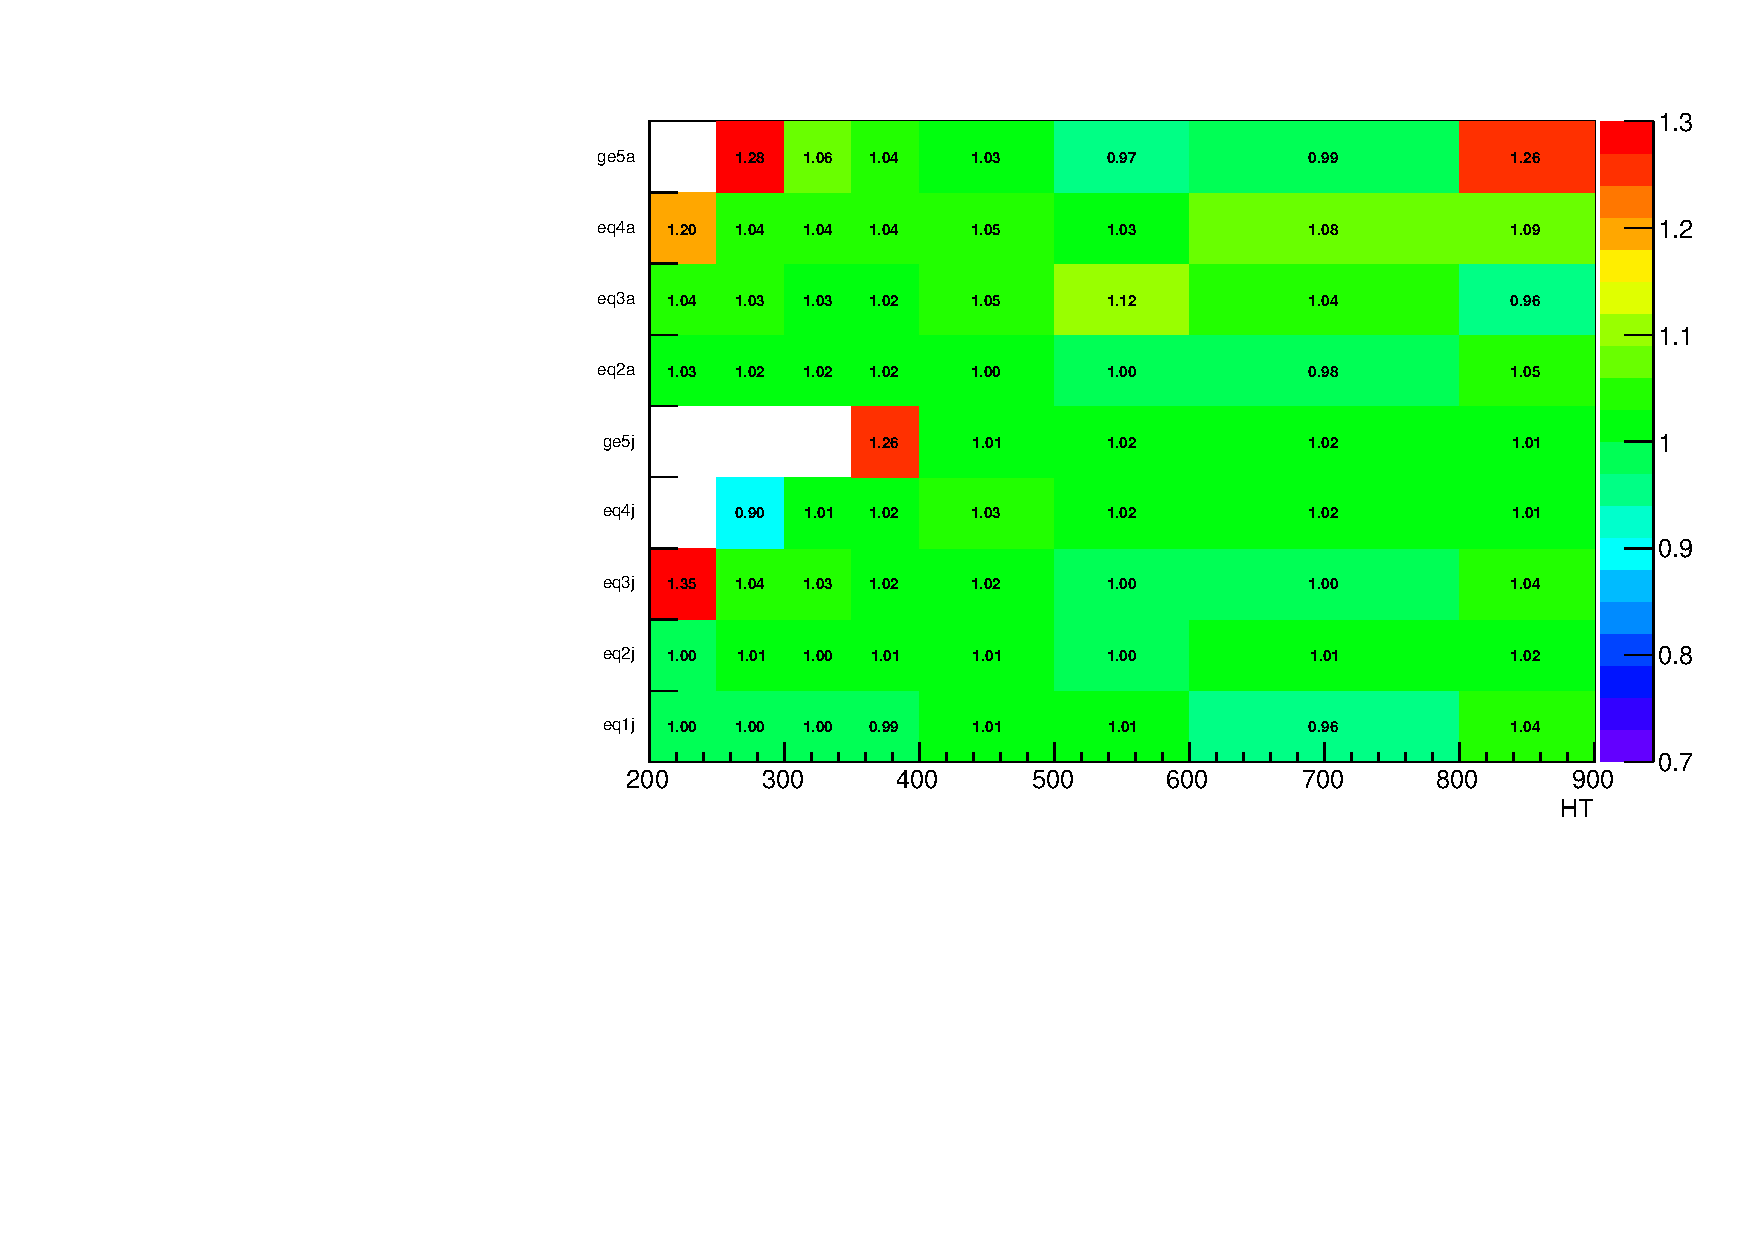
\includegraphics[width=0.4\textwidth]{Figures/backgroundPrediction/mcSystematics12p9fb/Zinv/muMergeNb/ratiotfh_ht_mht_alljecWeight_UpIncNb.pdf}
%   } ~~
%   \subfloat[JEC down variation]{
%     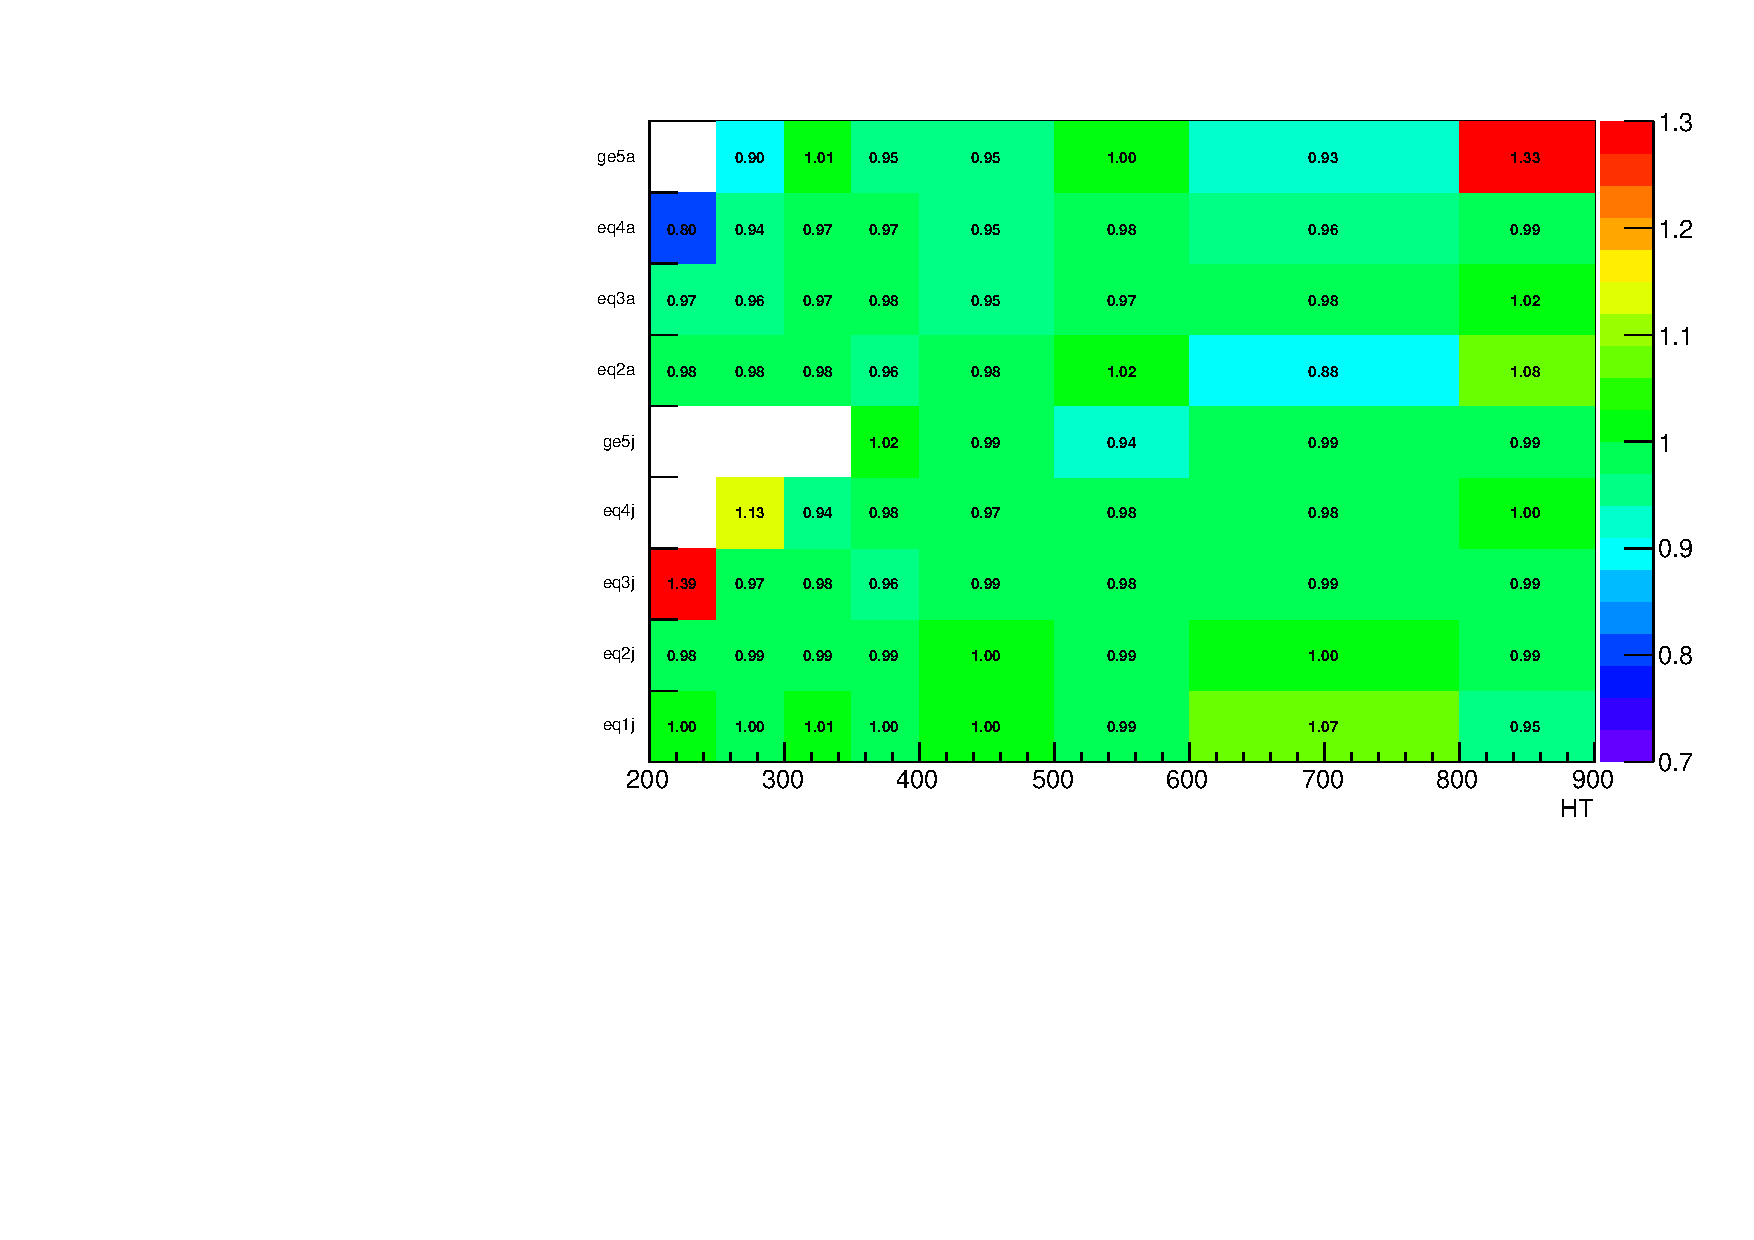
\includegraphics[width=0.4\textwidth]{Figures/backgroundPrediction/mcSystematics12p9fb/Zinv/muMergeNb/ratiotfh_ht_mht_alljecWeight_DownIncNb.pdf}
%   }\\
%
%   \caption{\label{fig:tfSyst_jec_muToZinv} The relative change in the
%   $\mj \rightarrow (\znunu)$ transfer
%   factors when varying JEC in MC within its uncertainties, as a function of \scalht and jet category. 
%   Variations corresponding to $+1\sigma$ ($-1\sigma$) are shown in the left (right) figure. 
%   }
% \end{figure}
%
% \begin{figure}[!h]
%   \centering
%   \subfloat[JEC up variation]{
%     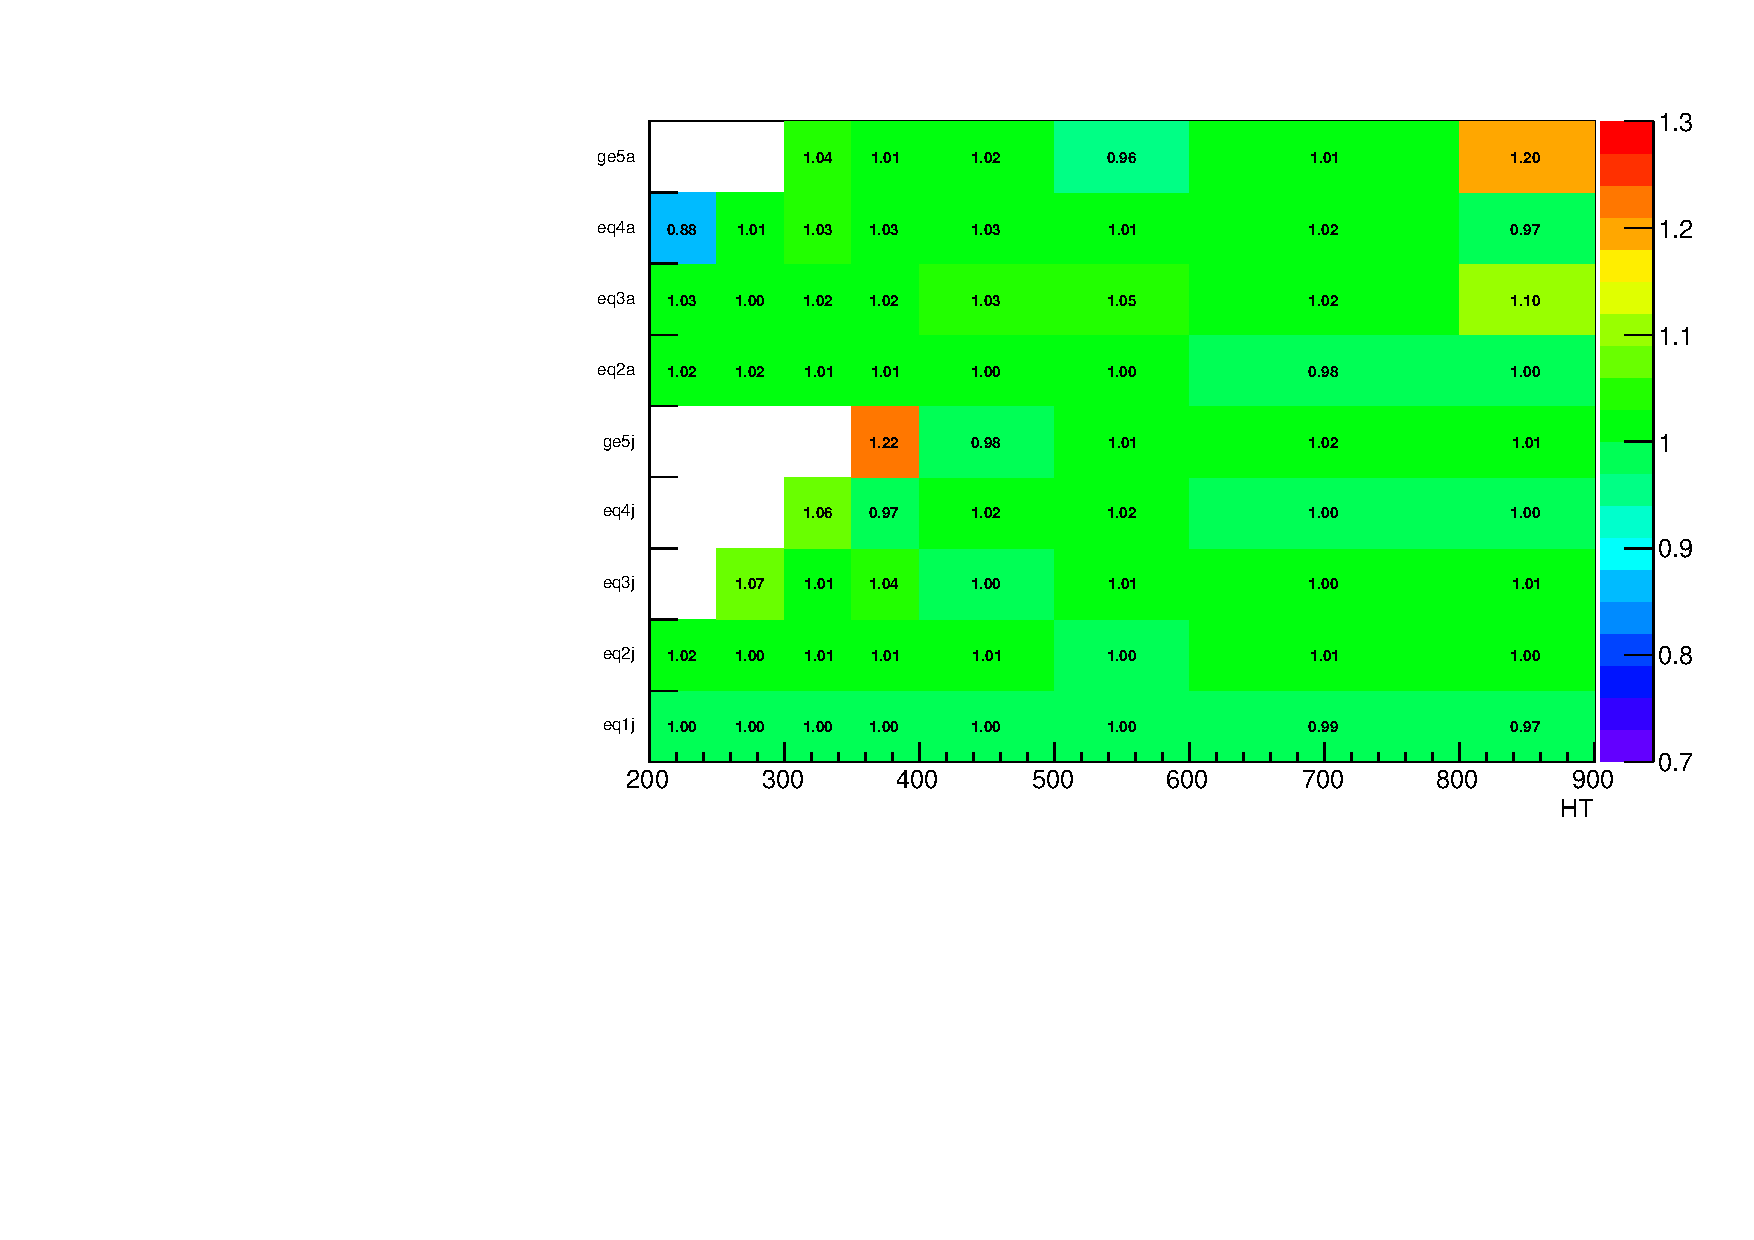
\includegraphics[width=0.4\textwidth]{Figures/backgroundPrediction/mcSystematics12p9fb/Zinv/mumuMergeNb/ratiotfh_ht_mht_alljecWeight_UpIncNb.pdf}
%   } ~~
%   \subfloat[JEC down variation]{
%     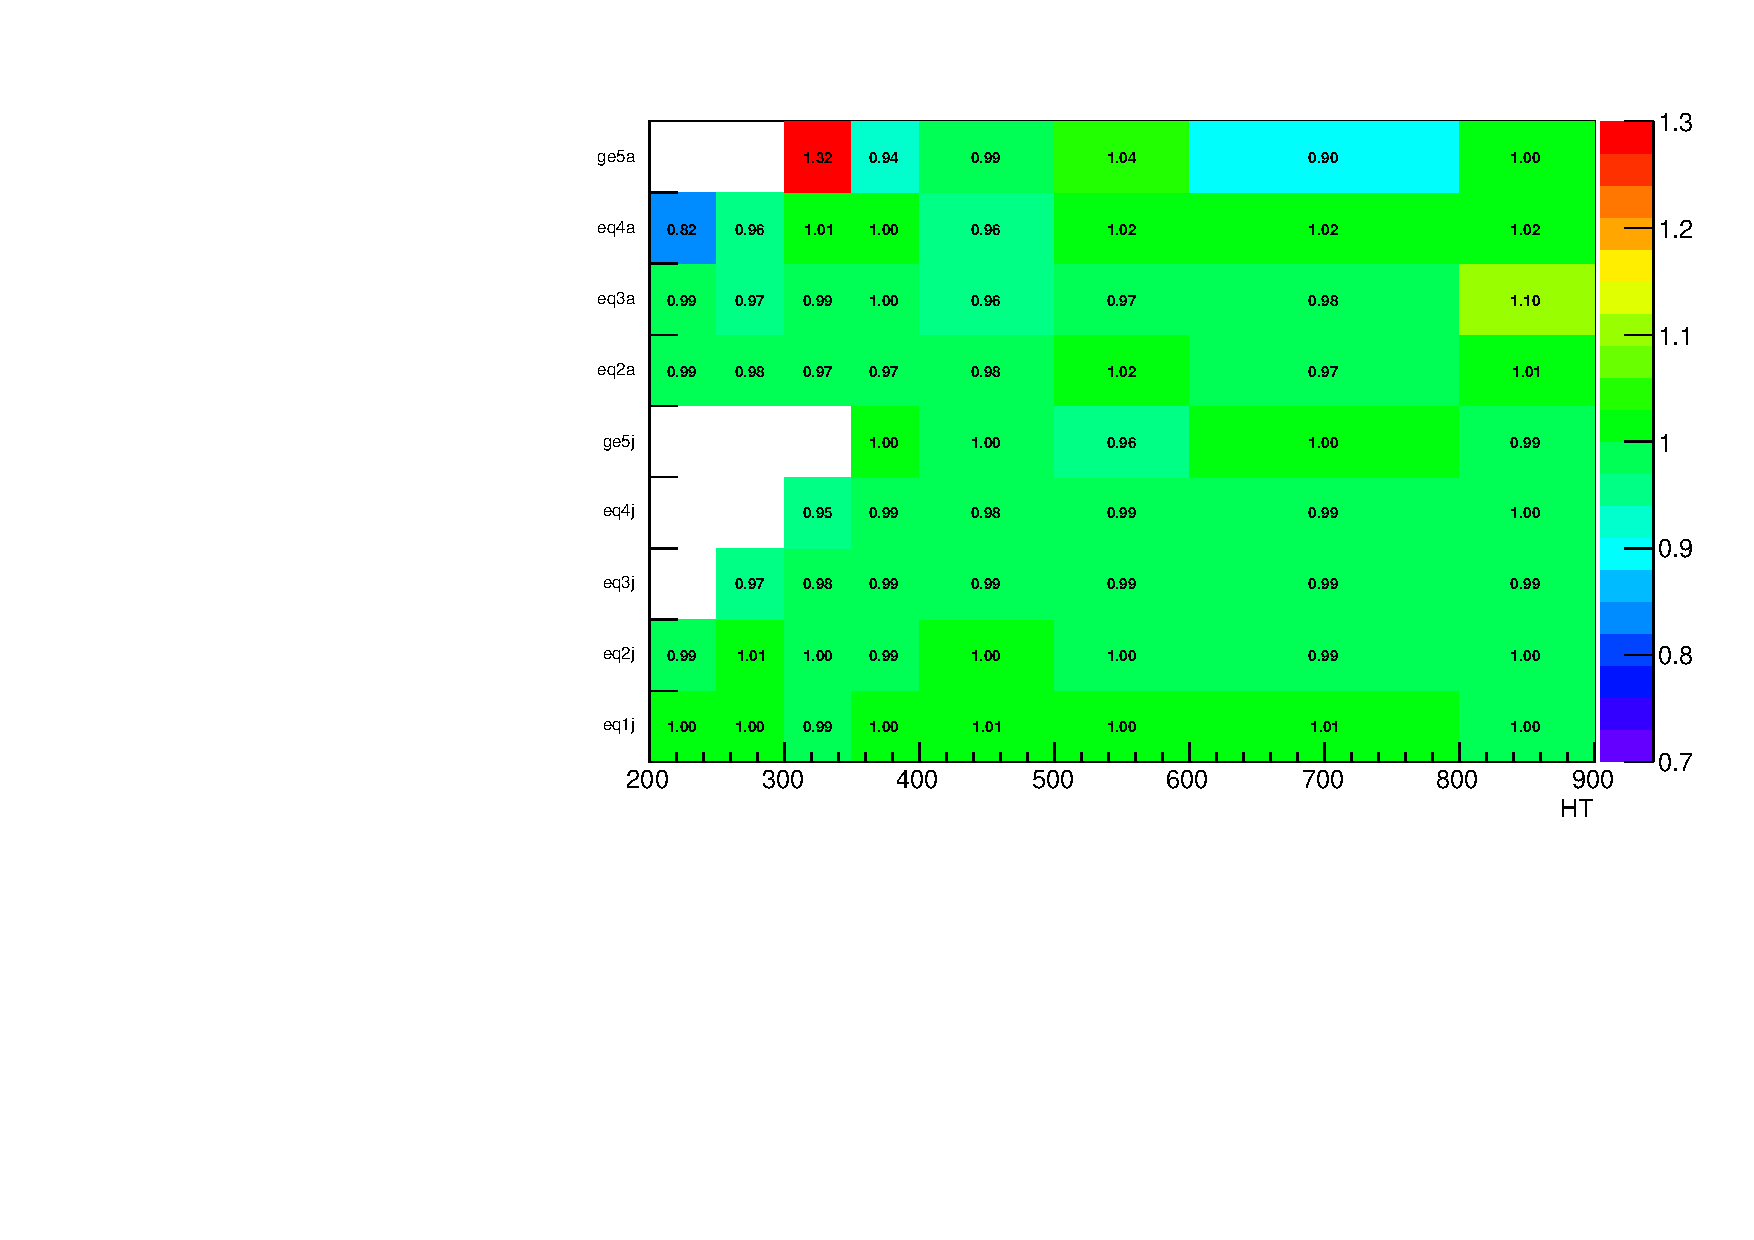
\includegraphics[width=0.4\textwidth]{Figures/backgroundPrediction/mcSystematics12p9fb/Zinv/mumuMergeNb/ratiotfh_ht_mht_alljecWeight_DownIncNb.pdf}
%   }\\
%
%   \caption{\label{fig:tfSyst_jec_mumuToZinv} The relative change in
%   the $\mmj \rightarrow (\znunu)$ transfer
%   factors when varying JEC in MC within its uncertainties, as a function of \scalht and jet category. 
%   Variations corresponding to $+1\sigma$ ($-1\sigma$) are shown in the left (right) figure. 
%   }
% \end{figure}
%
% \begin{figure}[!h]
%   \centering
%   \subfloat[JEC up variation]{
%     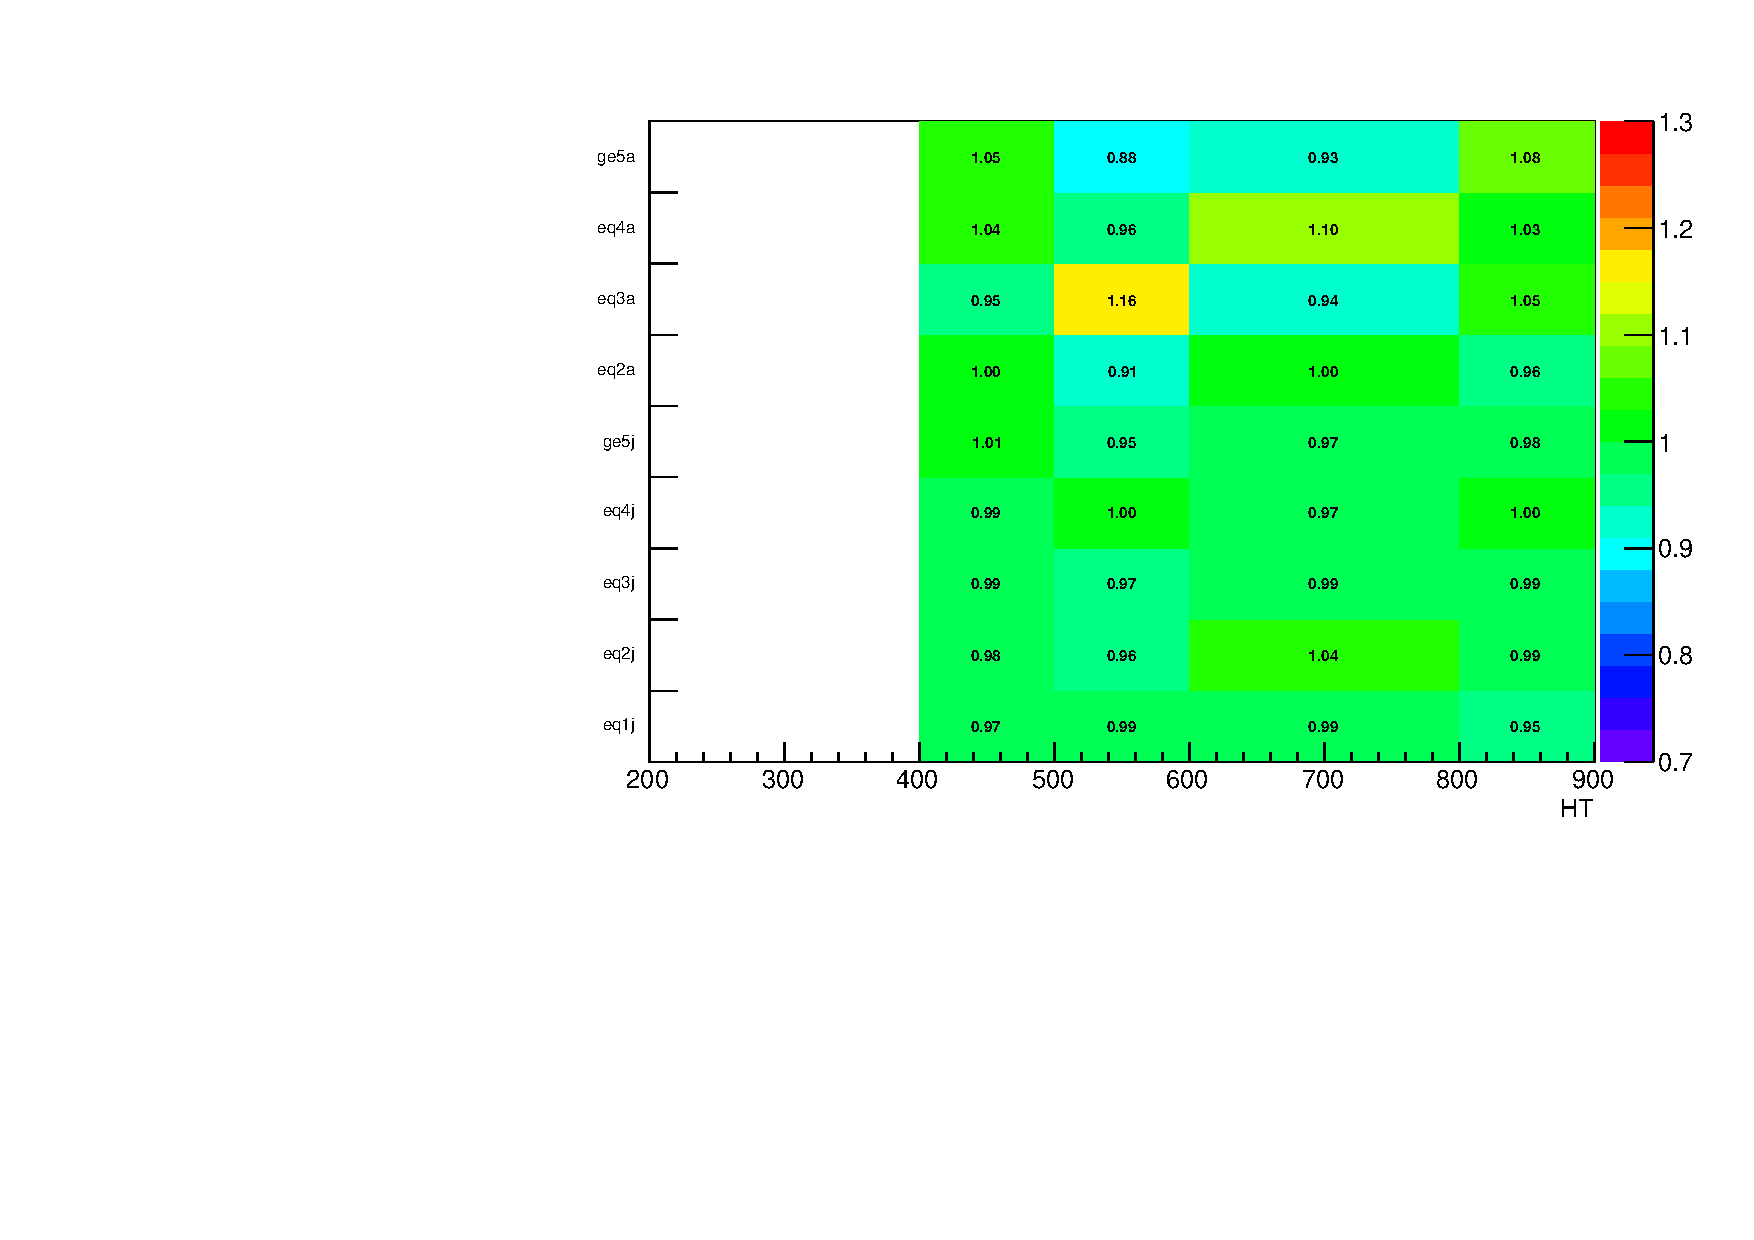
\includegraphics[width=0.4\textwidth]{Figures/backgroundPrediction/mcSystematics12p9fb/Zinv/gjMergeNb/ratiotfh_ht_mht_alljecWeight_UpIncNb.pdf}
%   } ~~
%   \subfloat[JEC down variation]{
%     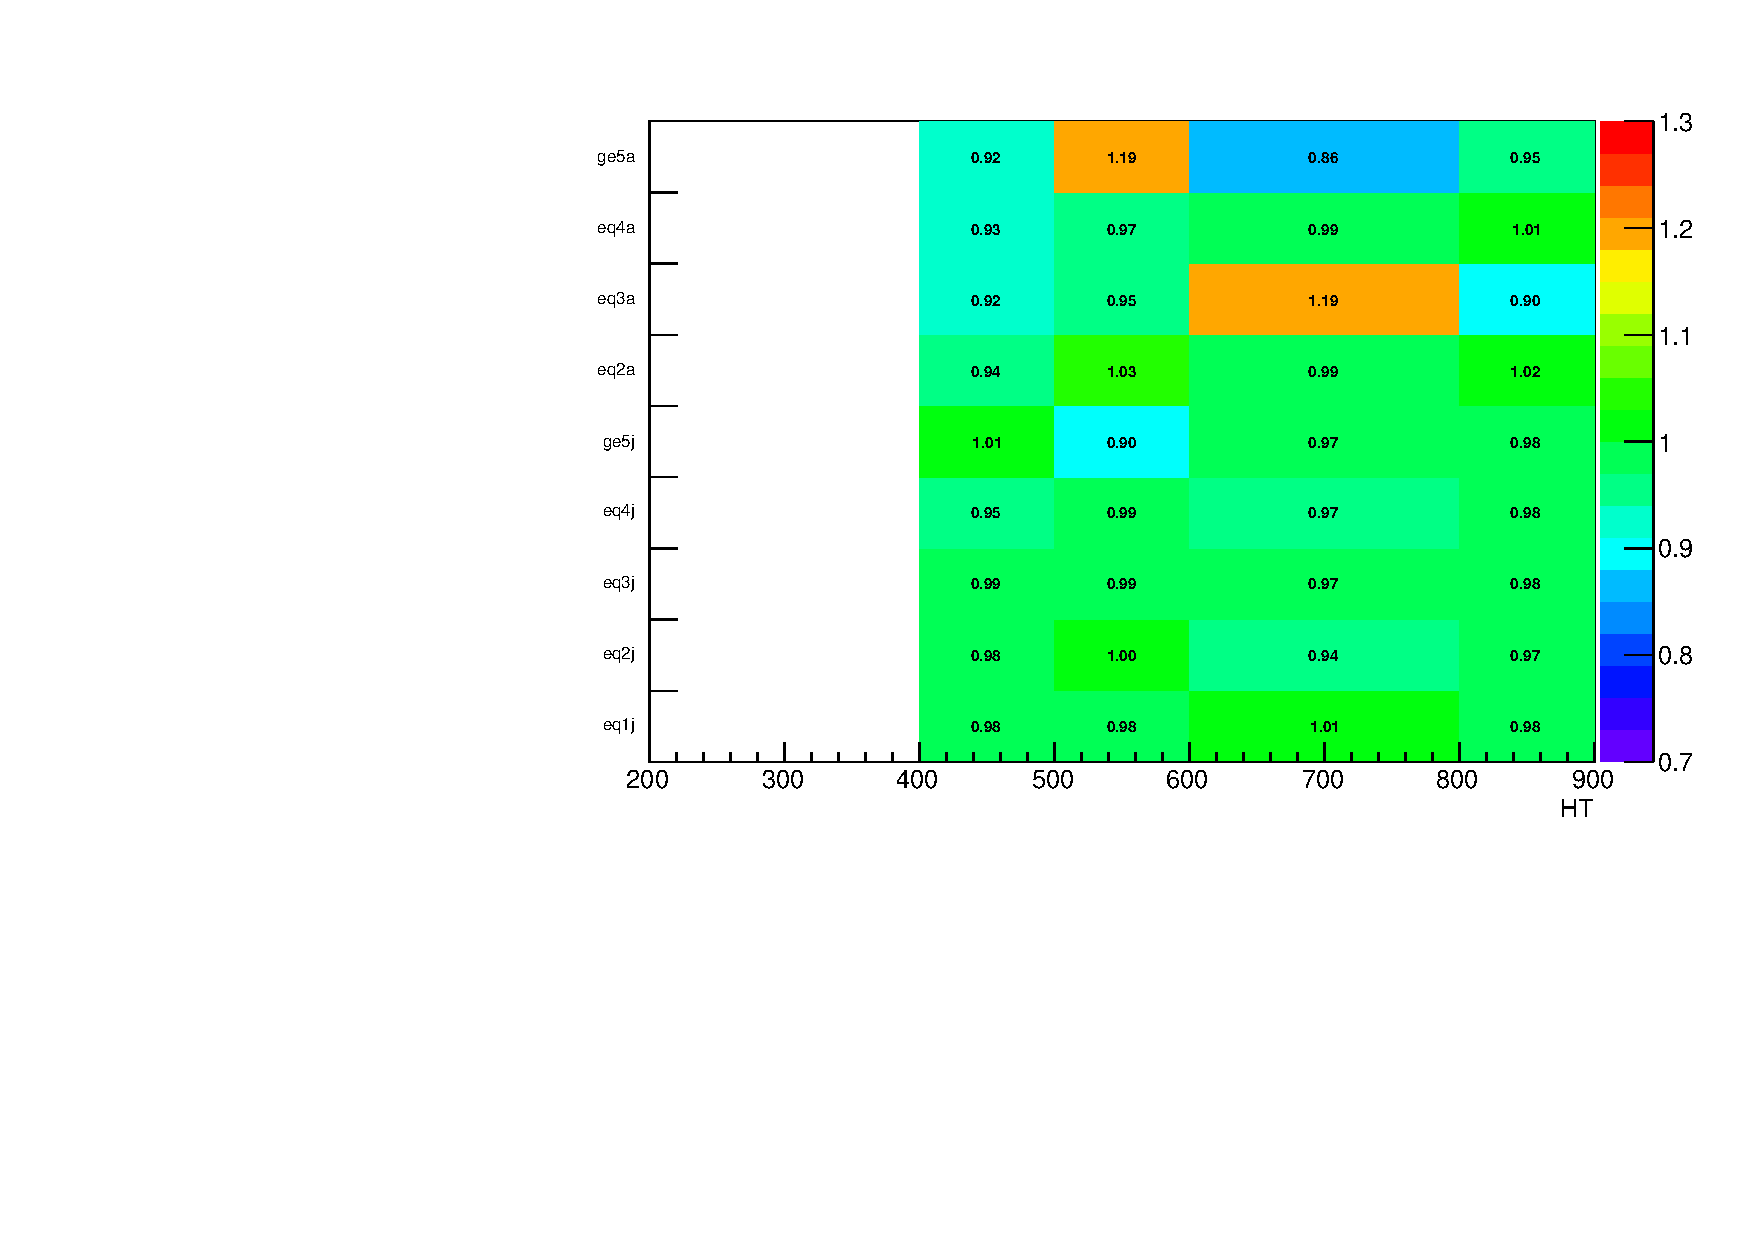
\includegraphics[width=0.4\textwidth]{Figures/backgroundPrediction/mcSystematics12p9fb/Zinv/gjMergeNb/ratiotfh_ht_mht_alljecWeight_DownIncNb.pdf}
%   }\\
%
%   \caption{\label{fig:tfSyst_jec_gjToZinv} The relative change in the
%   $\gj \rightarrow (\znunu)$ transfer
%   factors when varying JEC in MC within its uncertainties, as a function of \scalht and jet category. 
%   Variations corresponding to $+1\sigma$ ($-1\sigma$) are shown in the left (right) figure. 
%   }
% \end{figure}
%
% \begin{figure}[!h]
%   \centering
%   \subfloat[JEC up variation]{
%     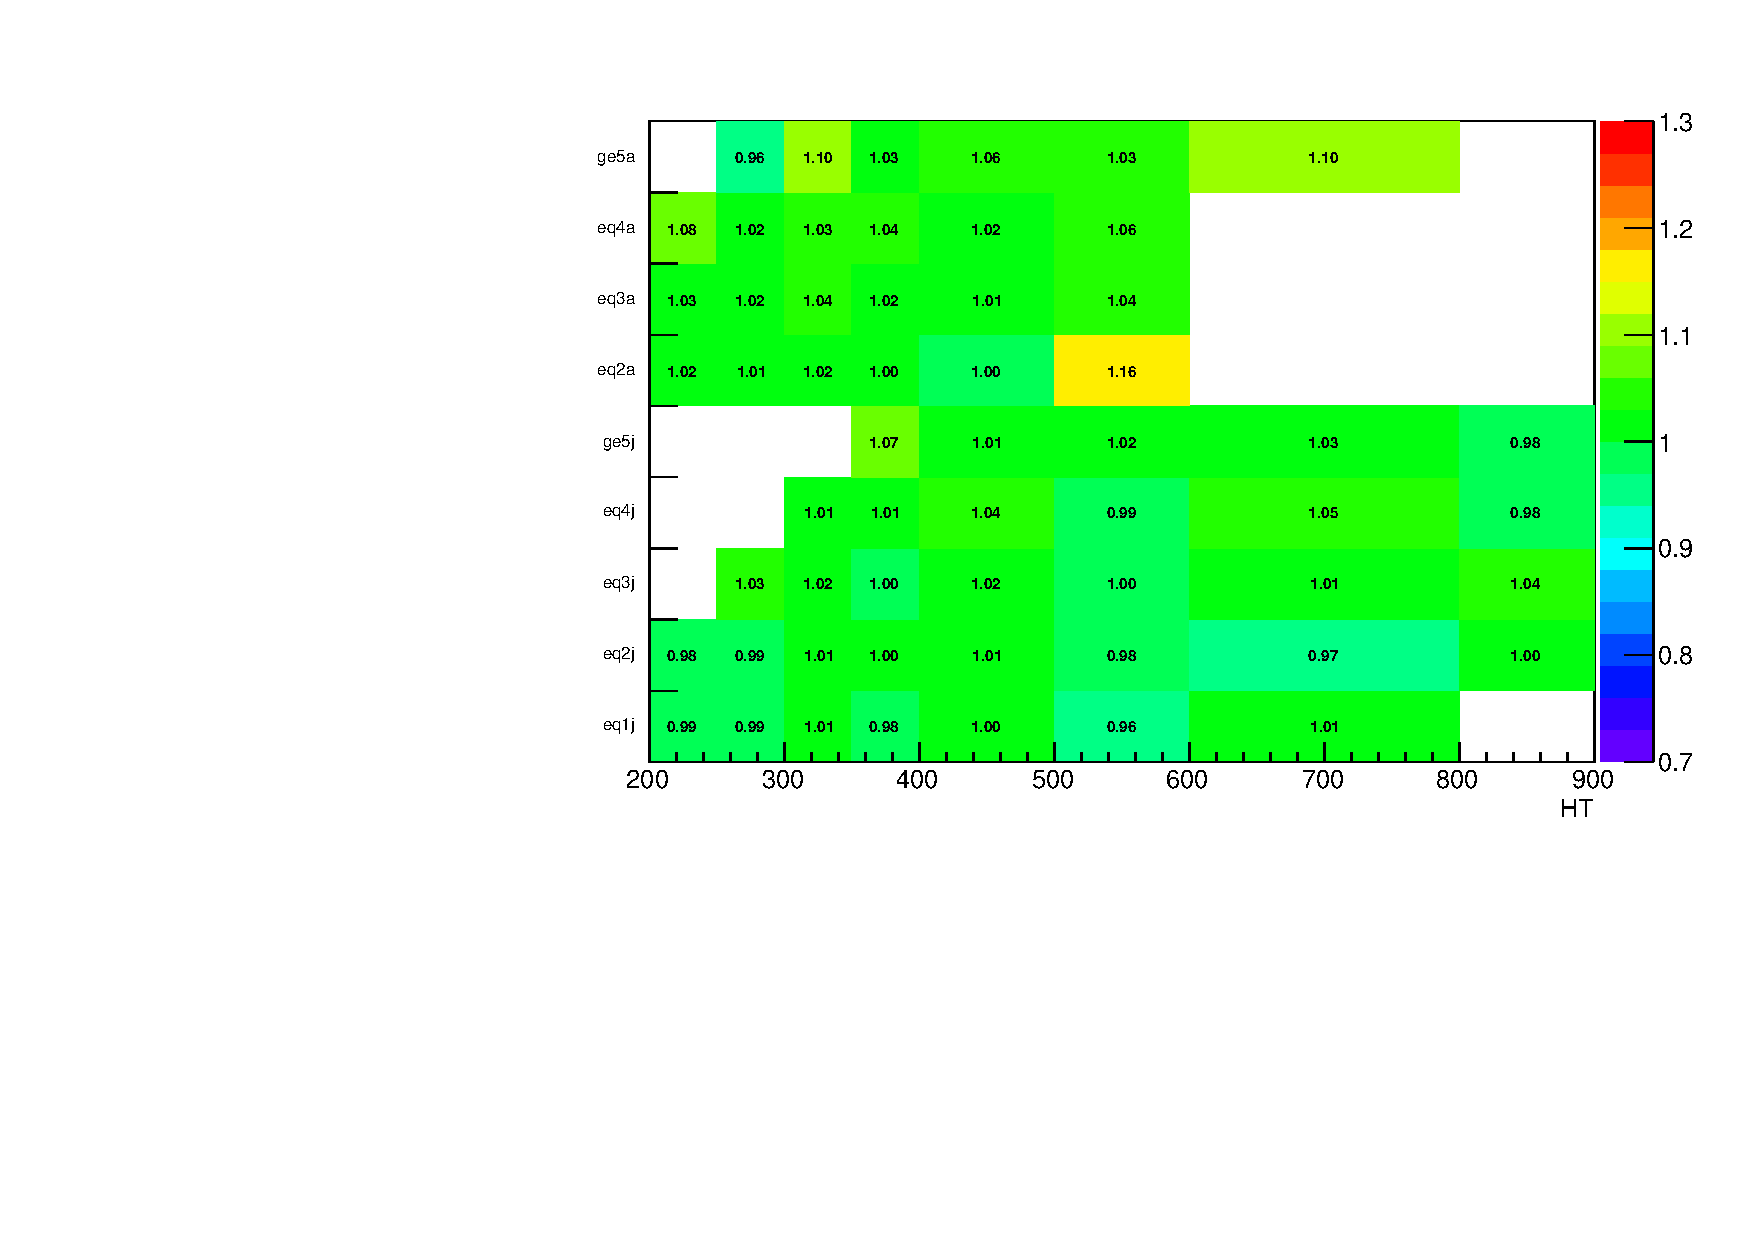
\includegraphics[width=0.4\textwidth]{Figures/backgroundPrediction/mcSystematics12p9fb/Ttw/muMergeNb/ratiotfh_ht_mht_alljecWeight_UpIncNb.pdf}
%   } ~~
%   \subfloat[JEC down variation]{
%     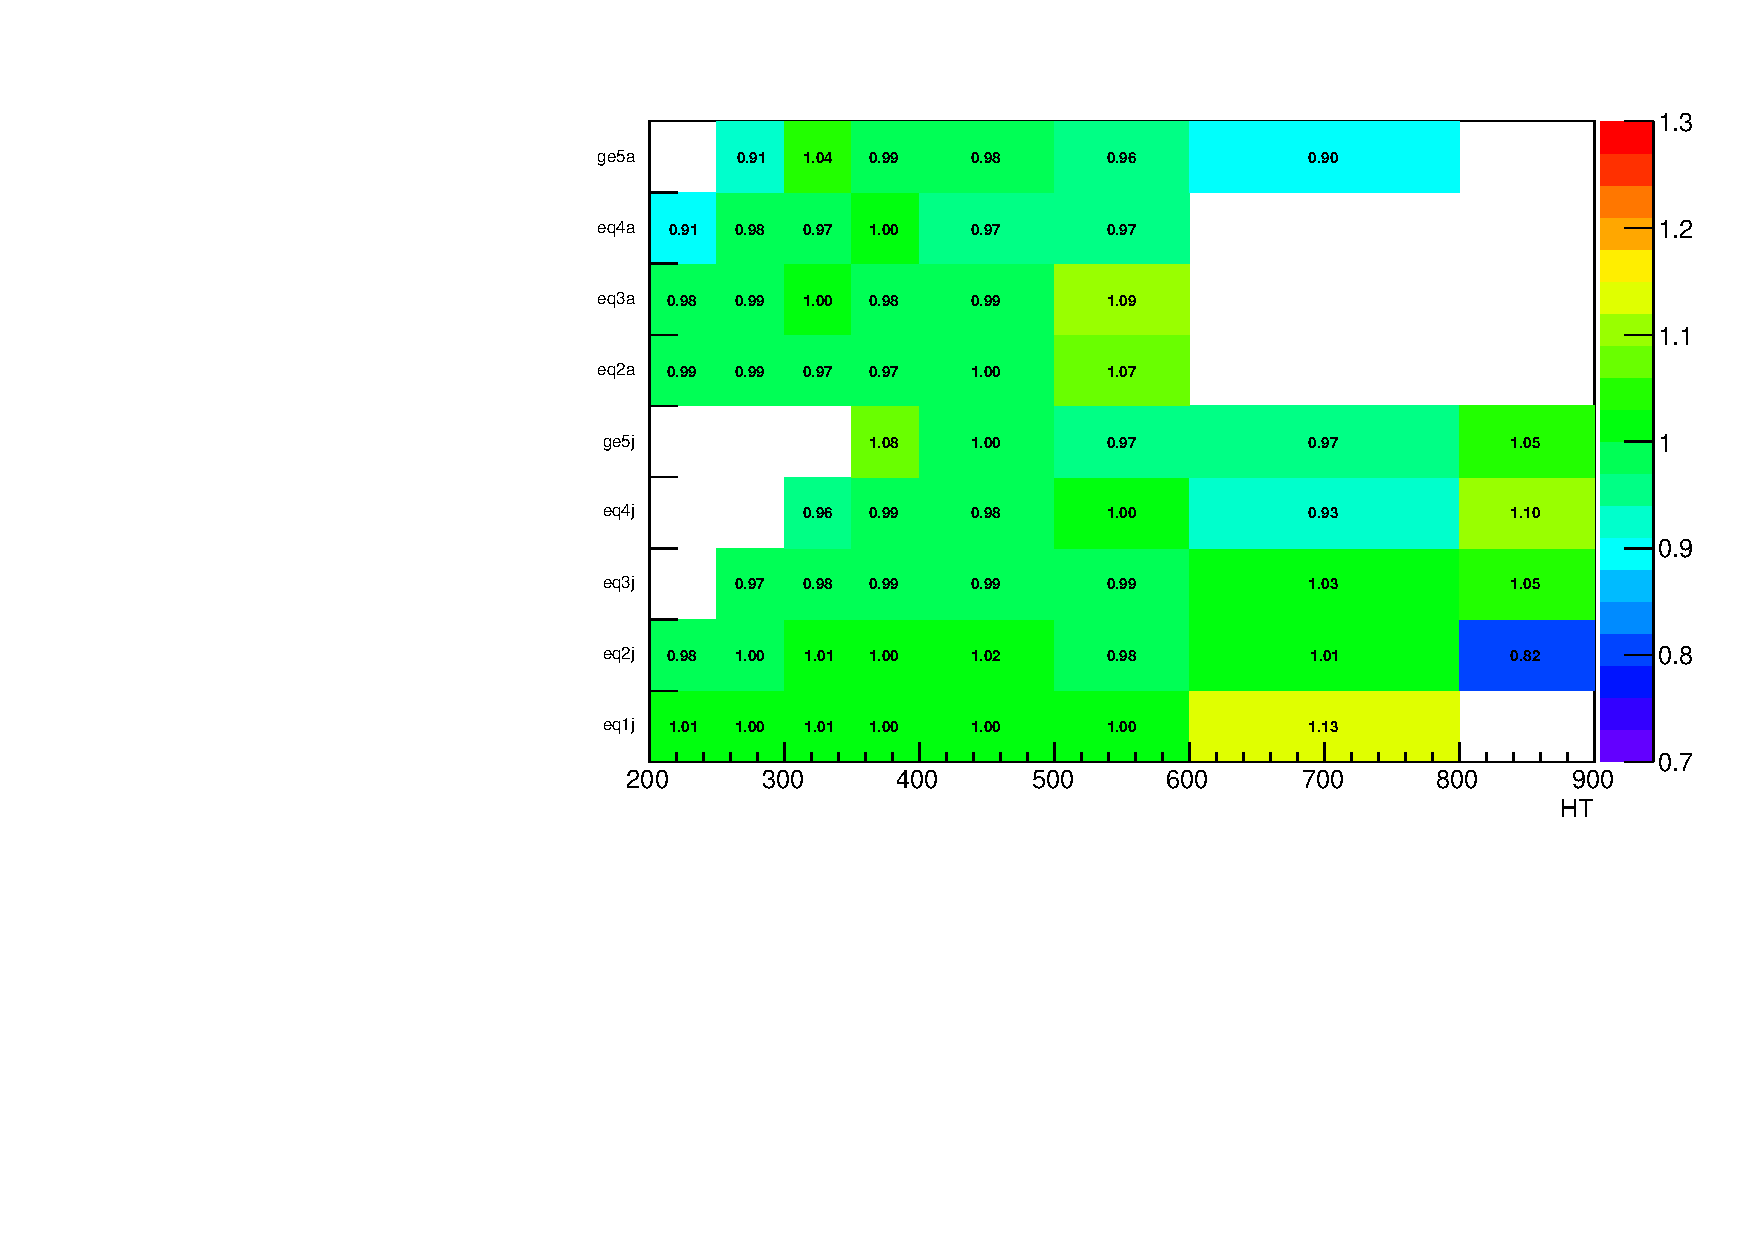
\includegraphics[width=0.4\textwidth]{Figures/backgroundPrediction/mcSystematics12p9fb/Ttw/muMergeNb/ratiotfh_ht_mht_alljecWeight_DownIncNb.pdf}
%   }\\
%
%   \caption{\label{fig:tfSyst_jec_muToTtw} The relative change in the
%   $\mj \rightarrow \mathrm{\ttbar+W}$ transfer
%   factors when varying JEC in MC within its uncertainties, as a function of \scalht and jet category. 
%   Variations corresponding to $+1\sigma$ ($-1\sigma$) are shown in the left (right) figure. 
%   }
% \end{figure}
%
% \clearpage
% \section{B-tagging efficiency}
%
% \begin{figure}[!h]
%   \centering
%   \subfloat[b tag SF (heavy) up variation]{
%     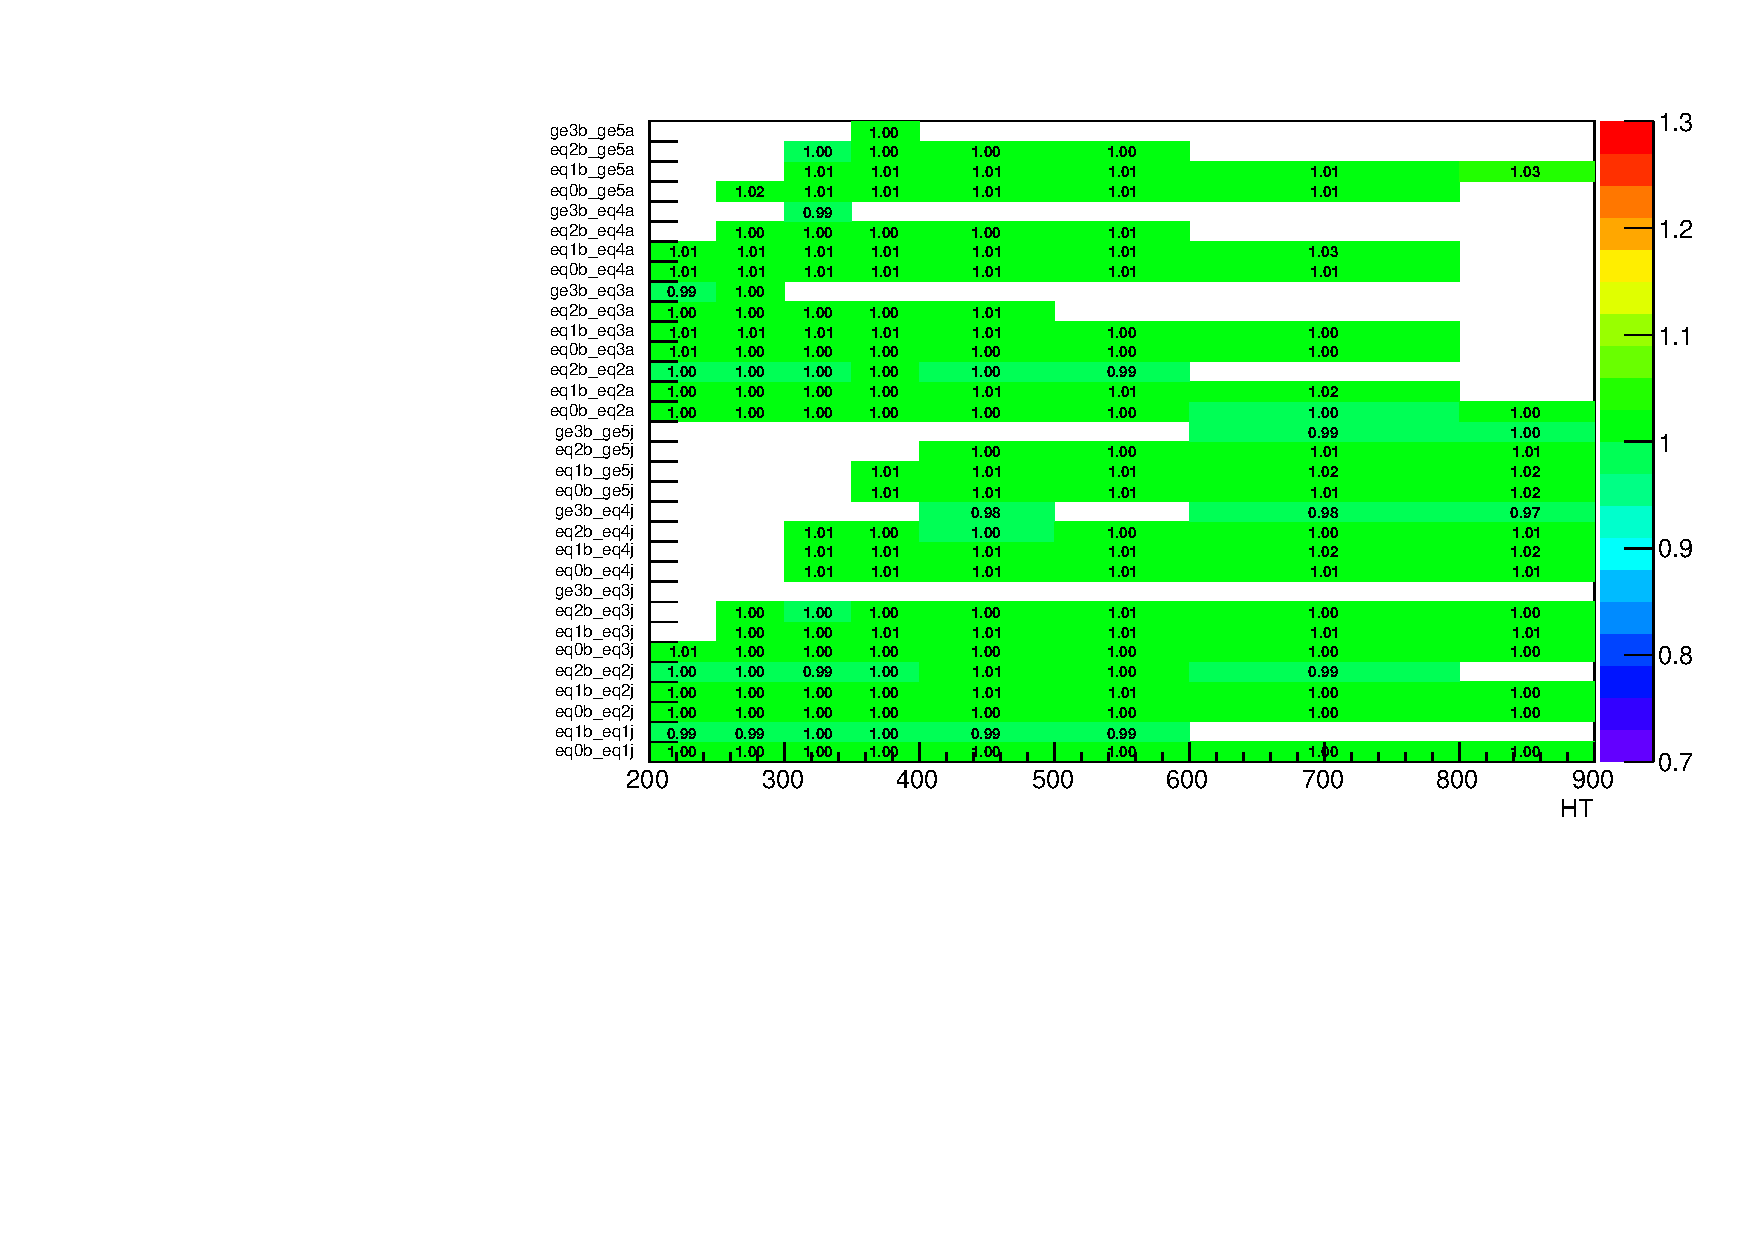
\includegraphics[width=0.4\textwidth]{Figures/backgroundPrediction/mcSystematics12p9fb/Zinv/mu/ratiotfh_ht_mht_allbsfWeight_Up.pdf}
%   } ~~
%   \subfloat[b tag SF (heavy) down variation]{
%     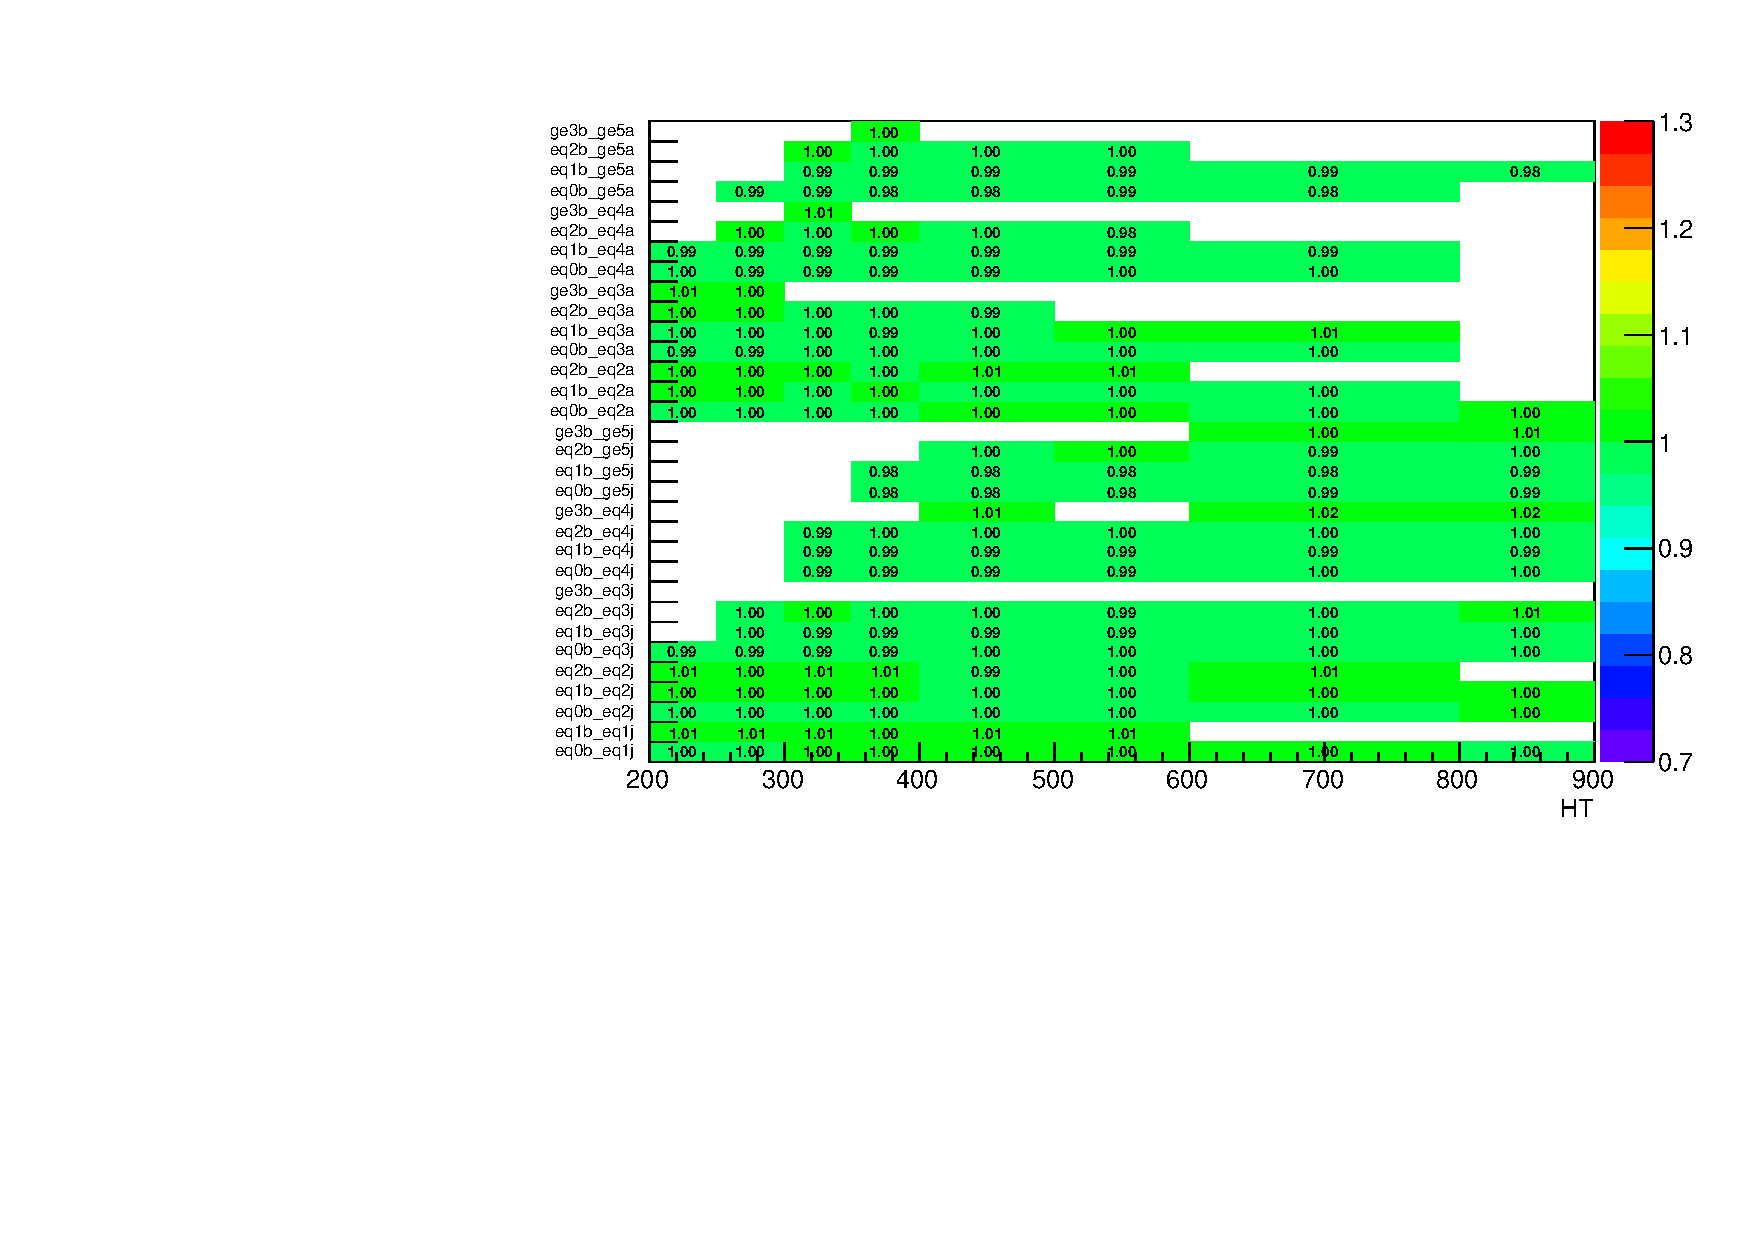
\includegraphics[width=0.4\textwidth]{Figures/backgroundPrediction/mcSystematics12p9fb/Zinv/mu/ratiotfh_ht_mht_allbsfWeight_Down.pdf}
%   }\\
%
%   \caption{\label{fig:tfSyst_bsf_muToZinv} The relative change in the
%   $\mj \rightarrow (\znunu)$ transfer
%   factors when varying b tag SF for heavy jets in MC within its uncertainties, as a function of \scalht and jet category. 
%   Variations corresponding to $+1\sigma$ ($-1\sigma$) are shown in the left (right) figure. 
%   }
% \end{figure}
%
% \begin{figure}[!h]
%   \centering
%   \subfloat[b tag SF (heavy) up variation]{
%     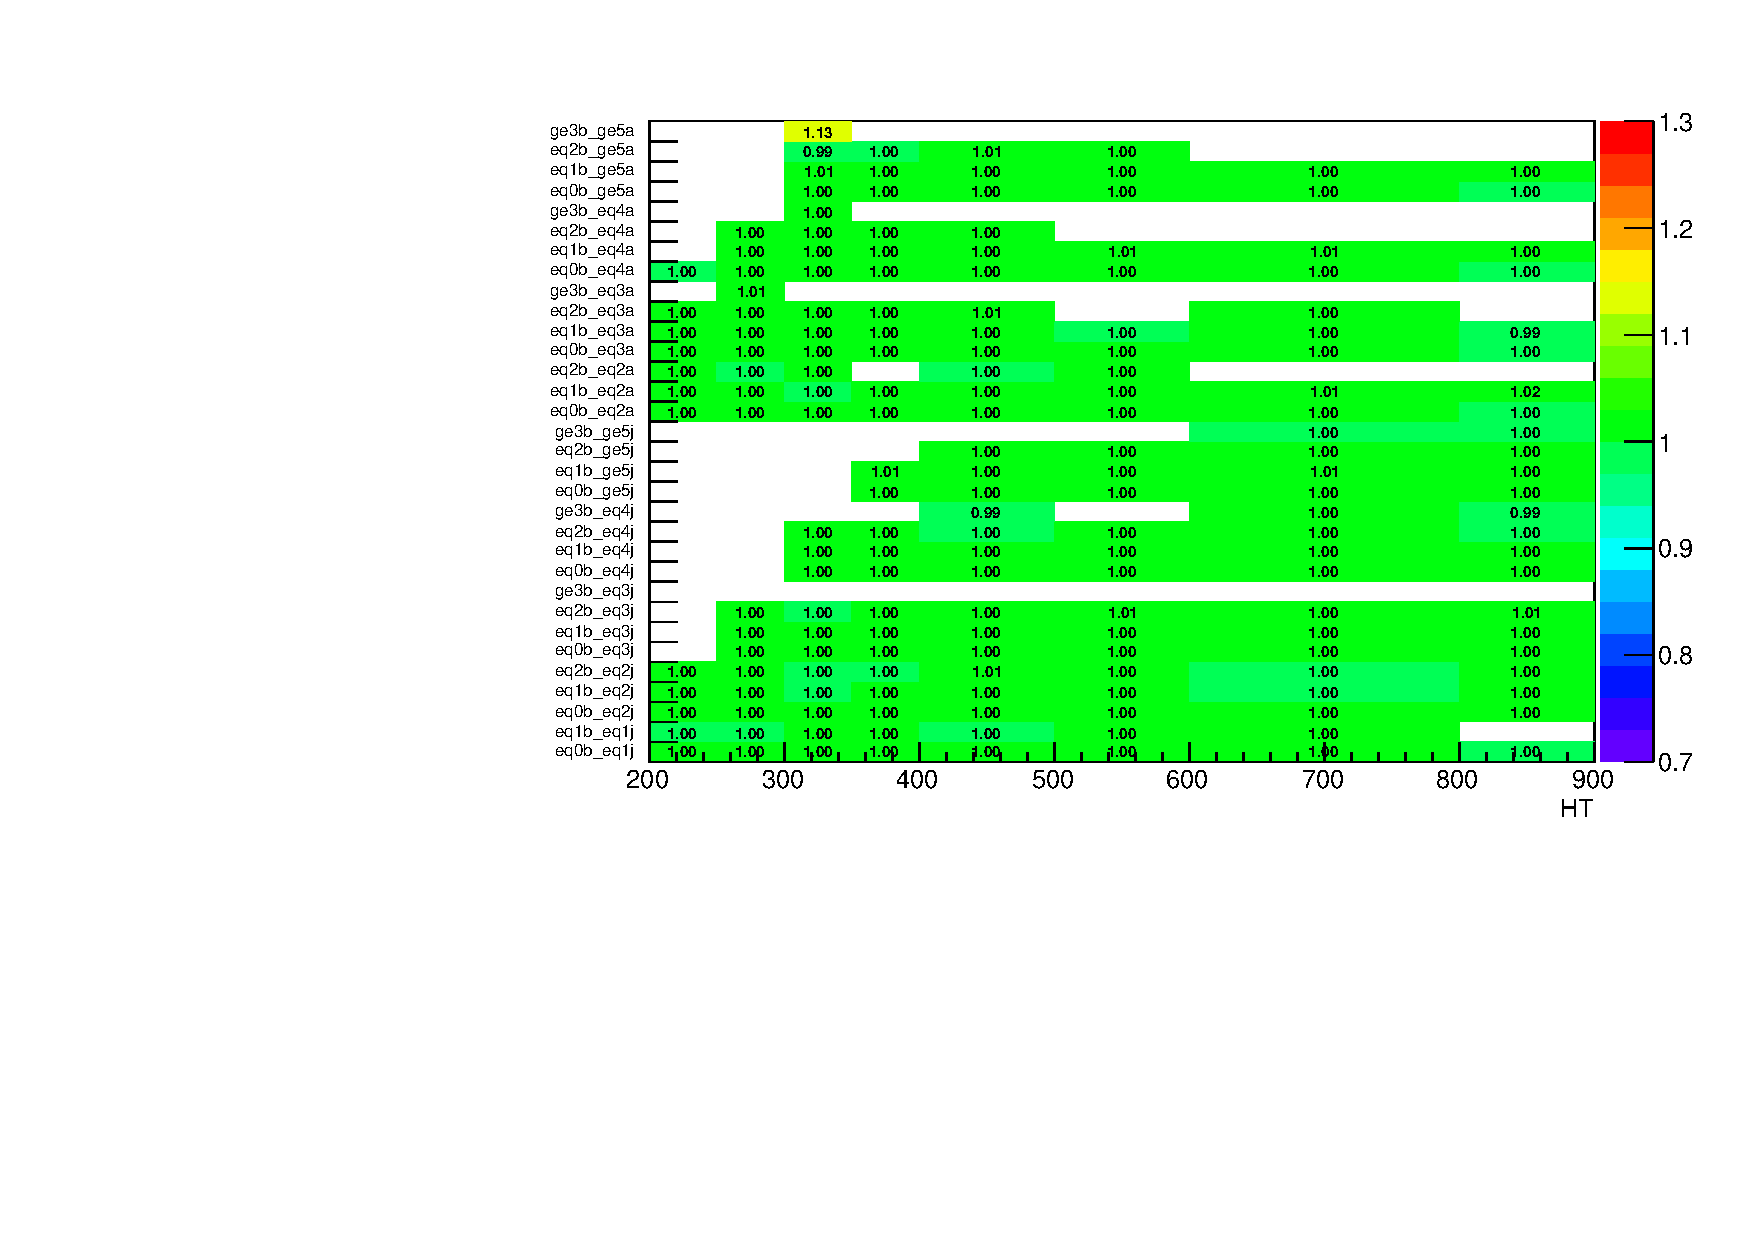
\includegraphics[width=0.4\textwidth]{Figures/backgroundPrediction/mcSystematics12p9fb/Zinv/mumu/ratiotfh_ht_mht_allbsfWeight_Up.pdf}
%   } ~~
%   \subfloat[b tag SF (heavy) down variation]{
%     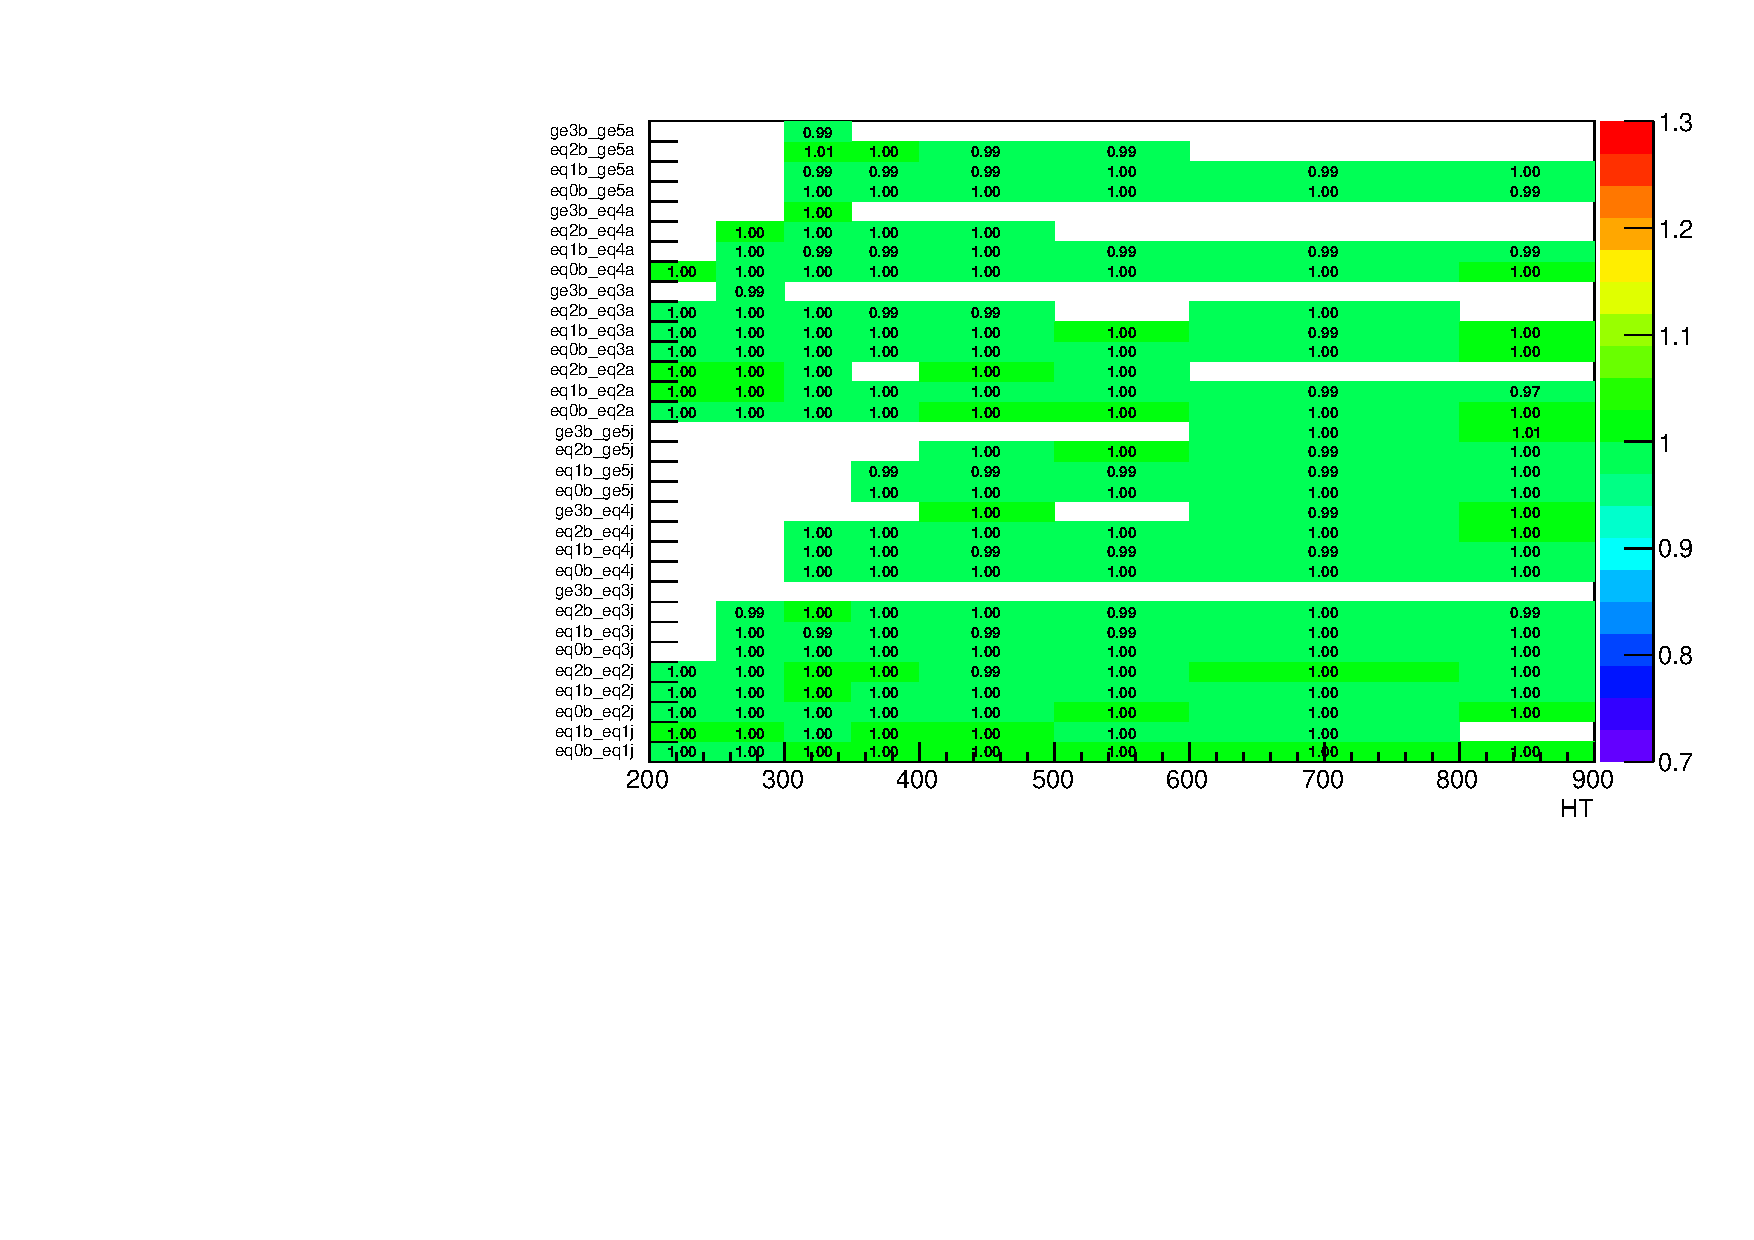
\includegraphics[width=0.4\textwidth]{Figures/backgroundPrediction/mcSystematics12p9fb/Zinv/mumu/ratiotfh_ht_mht_allbsfWeight_Down.pdf}
%   }\\
%
%   \caption{\label{fig:tfSyst_bsf_mumuToZinv} The relative change in
%   the $\mmj \rightarrow (\znunu)$ transfer
%   factors when varying b tag SF for heavy jets in MC within its uncertainties, as a function of \scalht and jet category. 
%   Variations corresponding to $+1\sigma$ ($-1\sigma$) are shown in the left (right) figure. 
%   }
% \end{figure}
%
% \begin{figure}[!h]
%   \centering
%   \subfloat[b tag SF (heavy) up variation]{
%     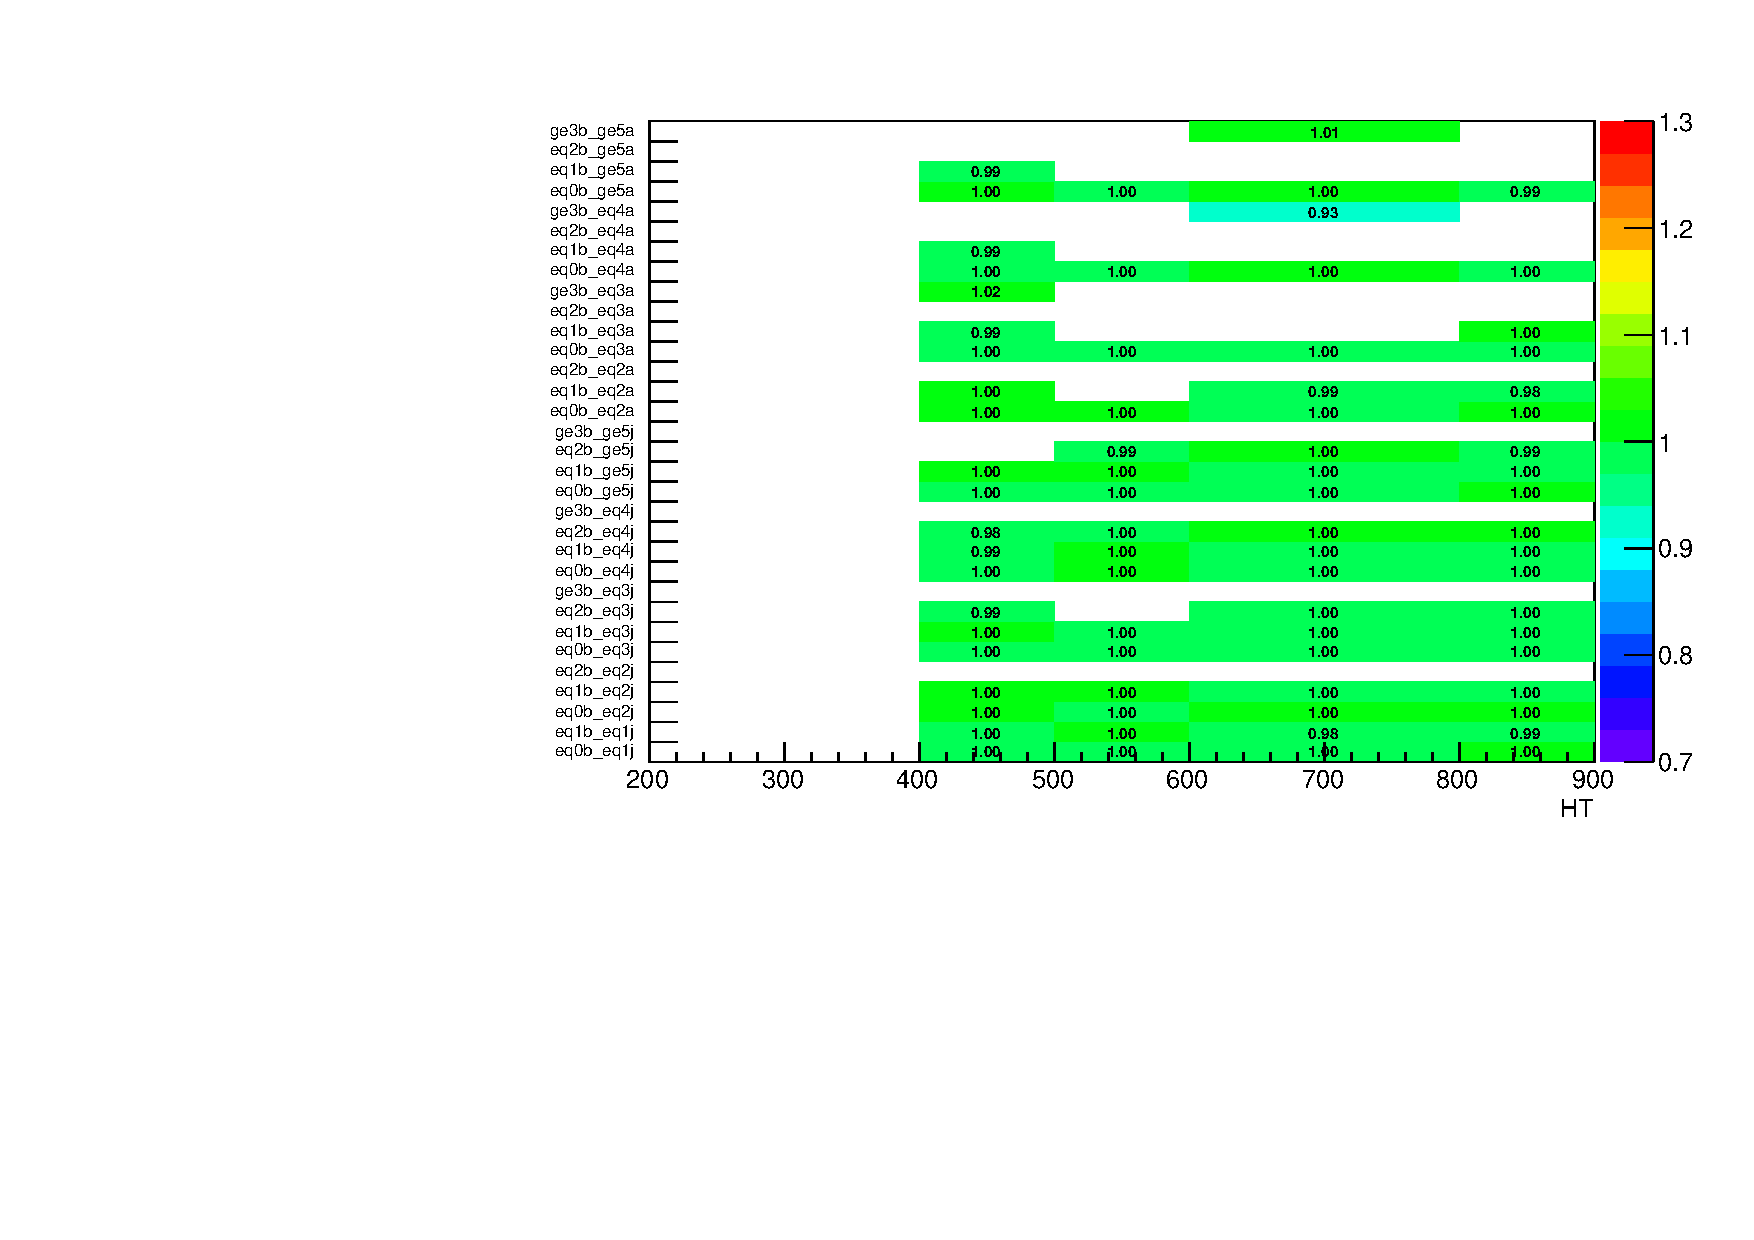
\includegraphics[width=0.4\textwidth]{Figures/backgroundPrediction/mcSystematics12p9fb/Zinv/gj/ratiotfh_ht_mht_allbsfWeight_Up.pdf}
%   } ~~
%   \subfloat[b tag SF (heavy) down variation]{
%     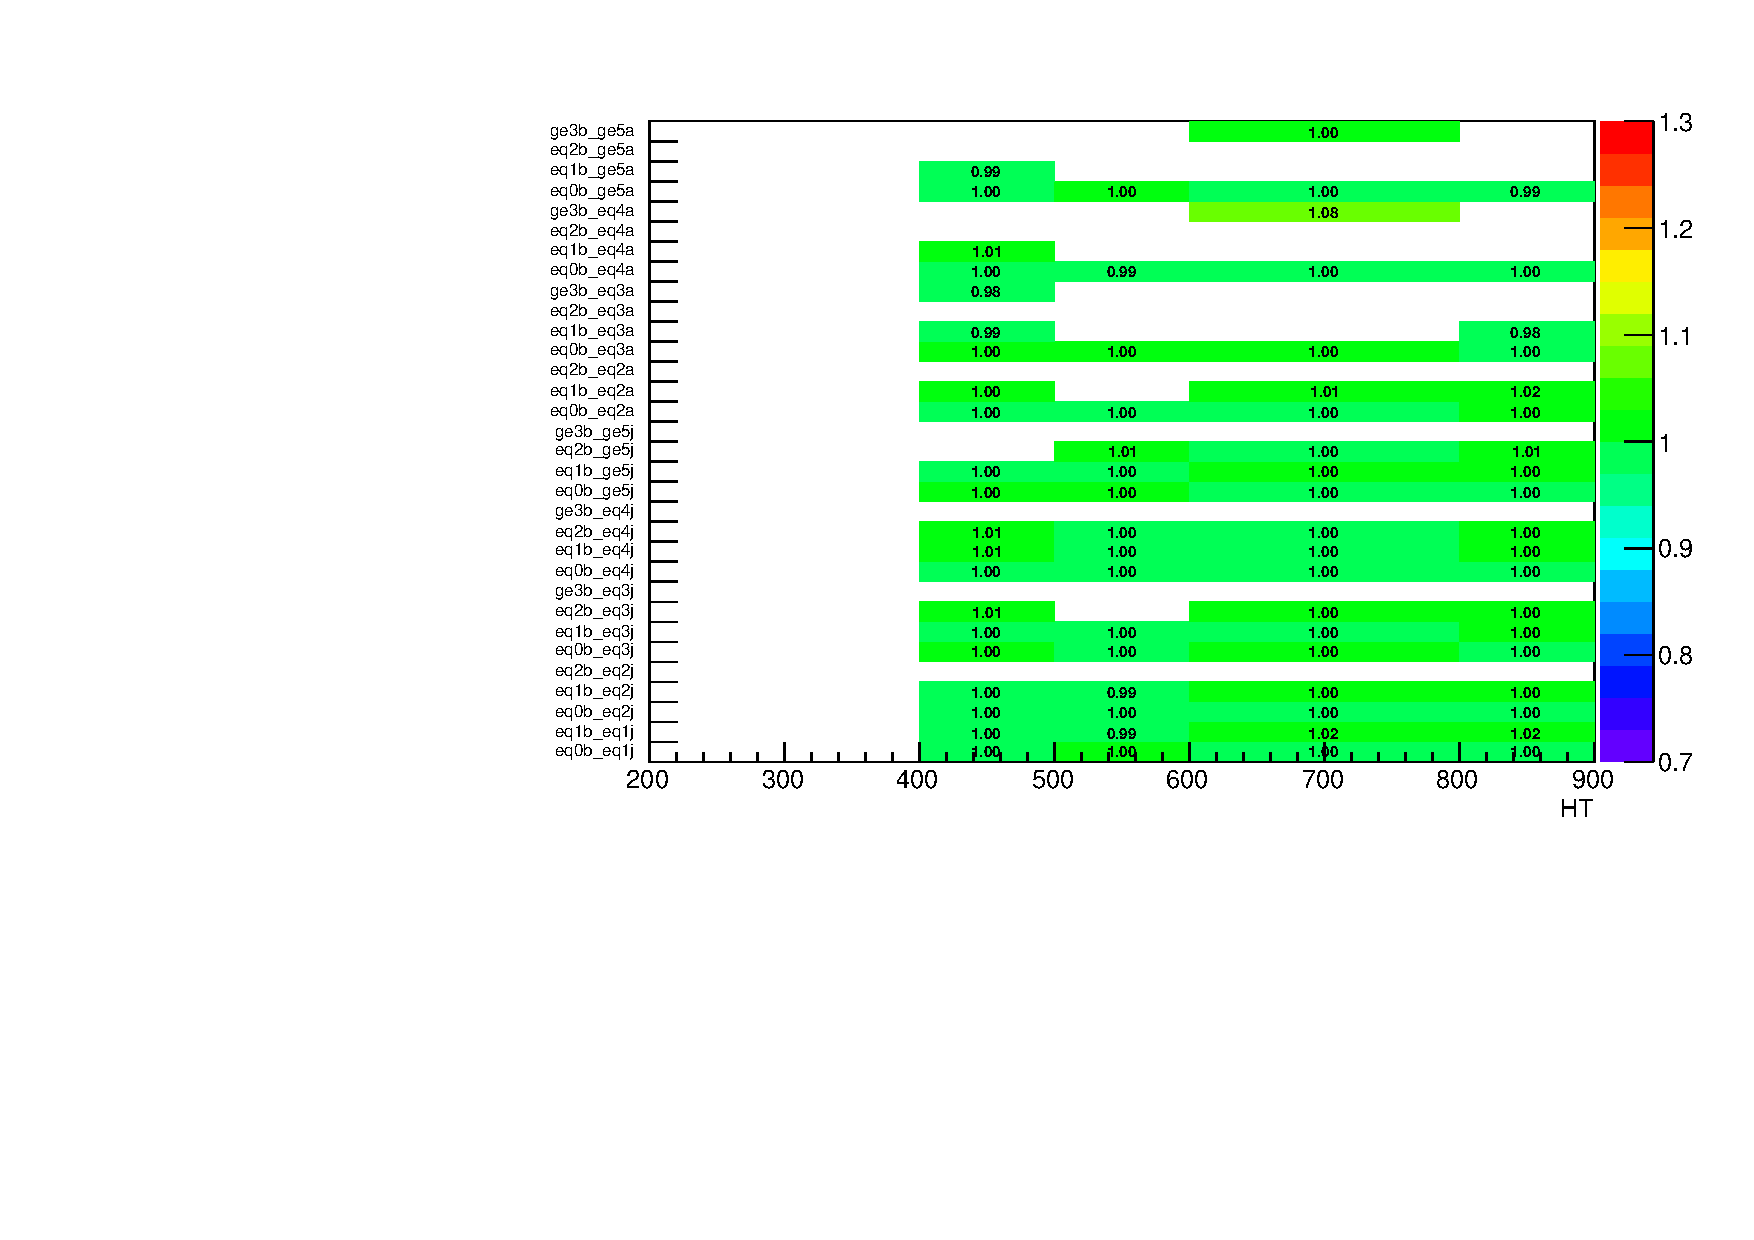
\includegraphics[width=0.4\textwidth]{Figures/backgroundPrediction/mcSystematics12p9fb/Zinv/gj/ratiotfh_ht_mht_allbsfWeight_Down.pdf}
%   }\\
%
%   \caption{\label{fig:tfSyst_bsf_gjToZinv} The relative change in the
%   $\gj \rightarrow (\znunu)$ transfer
%   factors when varying b tag SF for heavy jets in MC within its uncertainties, as a function of \scalht and jet category. 
%   Variations corresponding to $+1\sigma$ ($-1\sigma$) are shown in the left (right) figure. 
%   }
% \end{figure}
%
% \begin{figure}[!h]
%   \centering
%   \subfloat[b tag SF (heavy) up variation]{
%     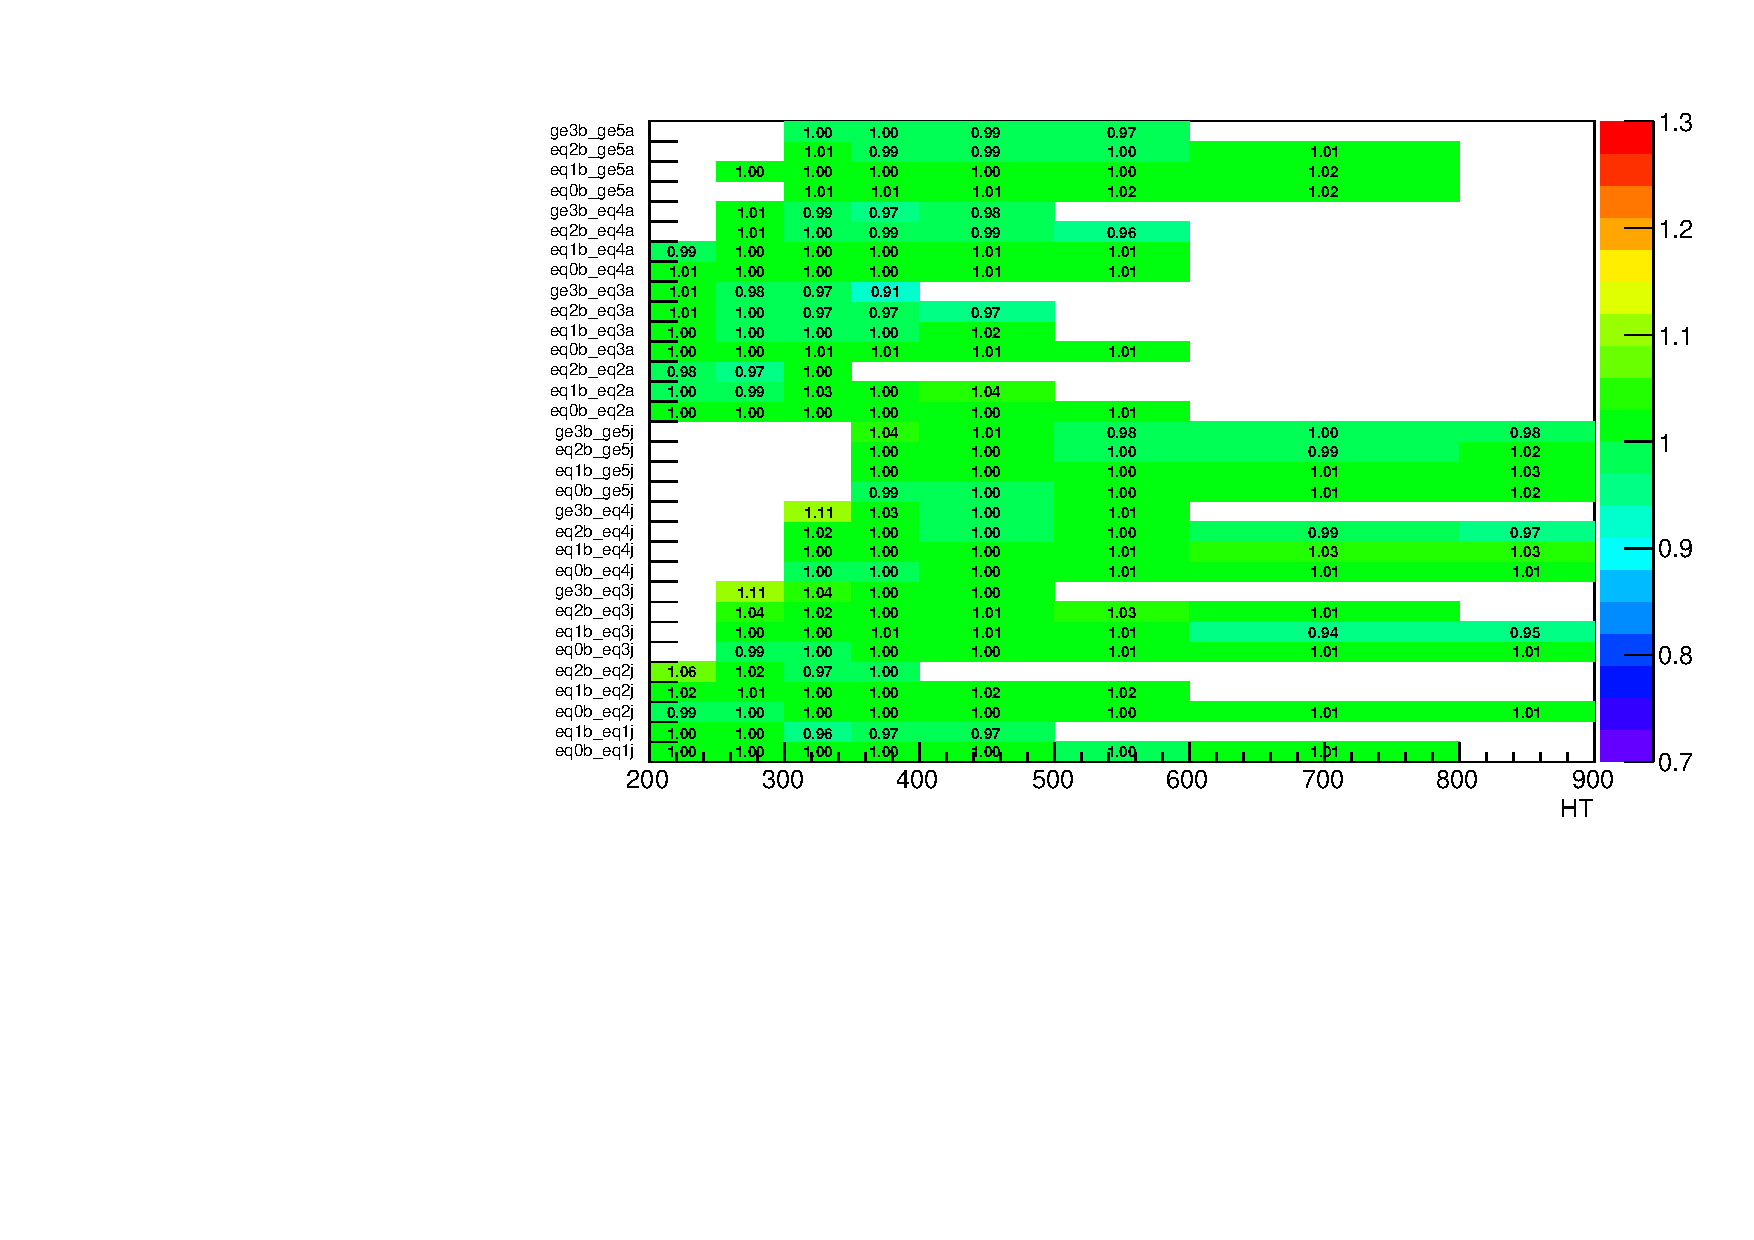
\includegraphics[width=0.4\textwidth]{Figures/backgroundPrediction/mcSystematics12p9fb/Ttw/mu/ratiotfh_ht_mht_allbsfWeight_Up.pdf}
%   } ~~
%   \subfloat[b tag SF (heavy) down variation]{
%     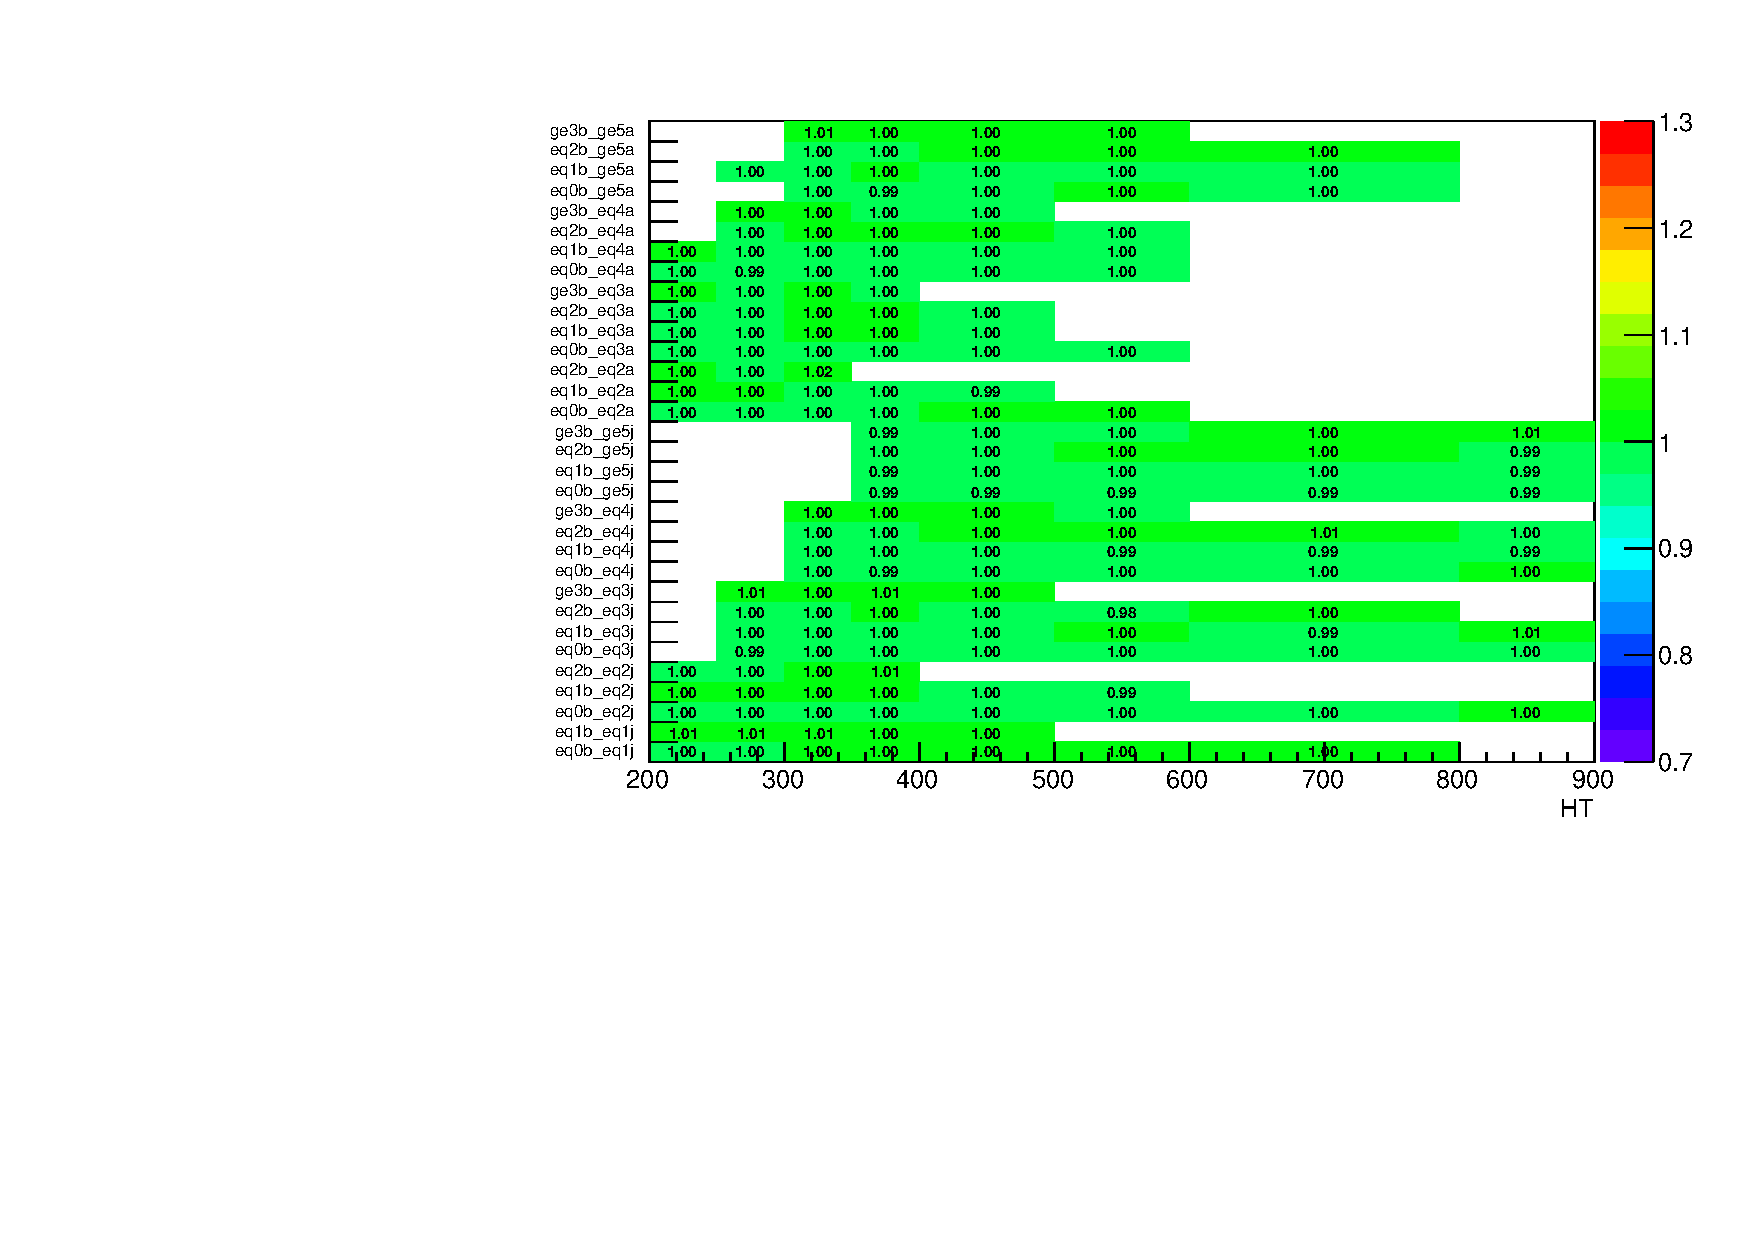
\includegraphics[width=0.4\textwidth]{Figures/backgroundPrediction/mcSystematics12p9fb/Ttw/mu/ratiotfh_ht_mht_allbsfWeight_Down.pdf}
%   }\\
%
%   \caption{\label{fig:tfSyst_bsf_muToTtw} The relative change in the $\mj \rightarrow \mathrm{tt+W}$ transfer
%   factors when varying b tag SF for heavy jets in MC within its uncertainties, as a function of \scalht and jet category. 
%   Variations corresponding to $+1\sigma$ ($-1\sigma$) are shown in the left (right) figure. 
%   }
% \end{figure}
%
% \begin{figure}[!h]
%   \centering
%   \subfloat[b tag SF (light) up variation]{
%     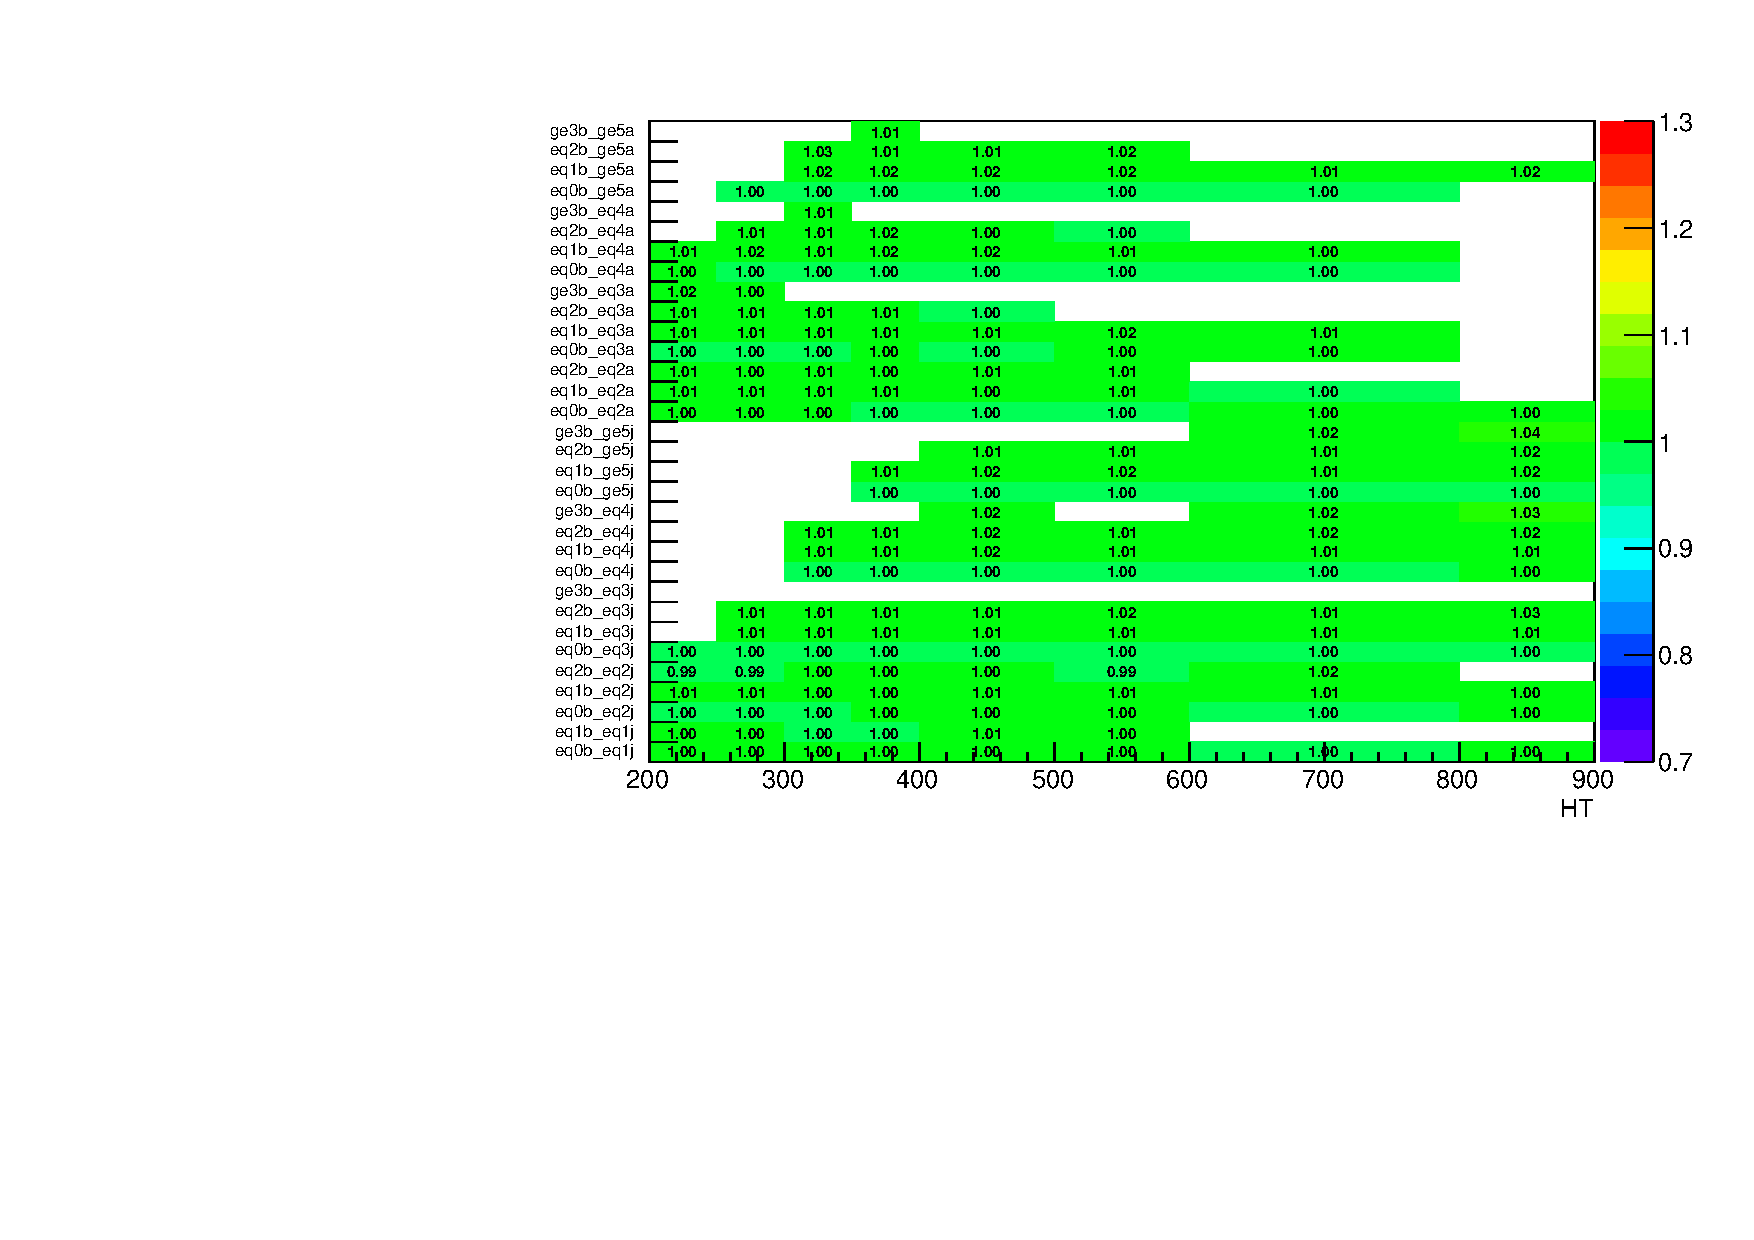
\includegraphics[width=0.4\textwidth]{Figures/backgroundPrediction/mcSystematics12p9fb/Zinv/mu/ratiotfh_ht_mht_allbsfLightWeight_Up.pdf}
%   } ~~
%   \subfloat[b tag SF (light) down variation]{
%     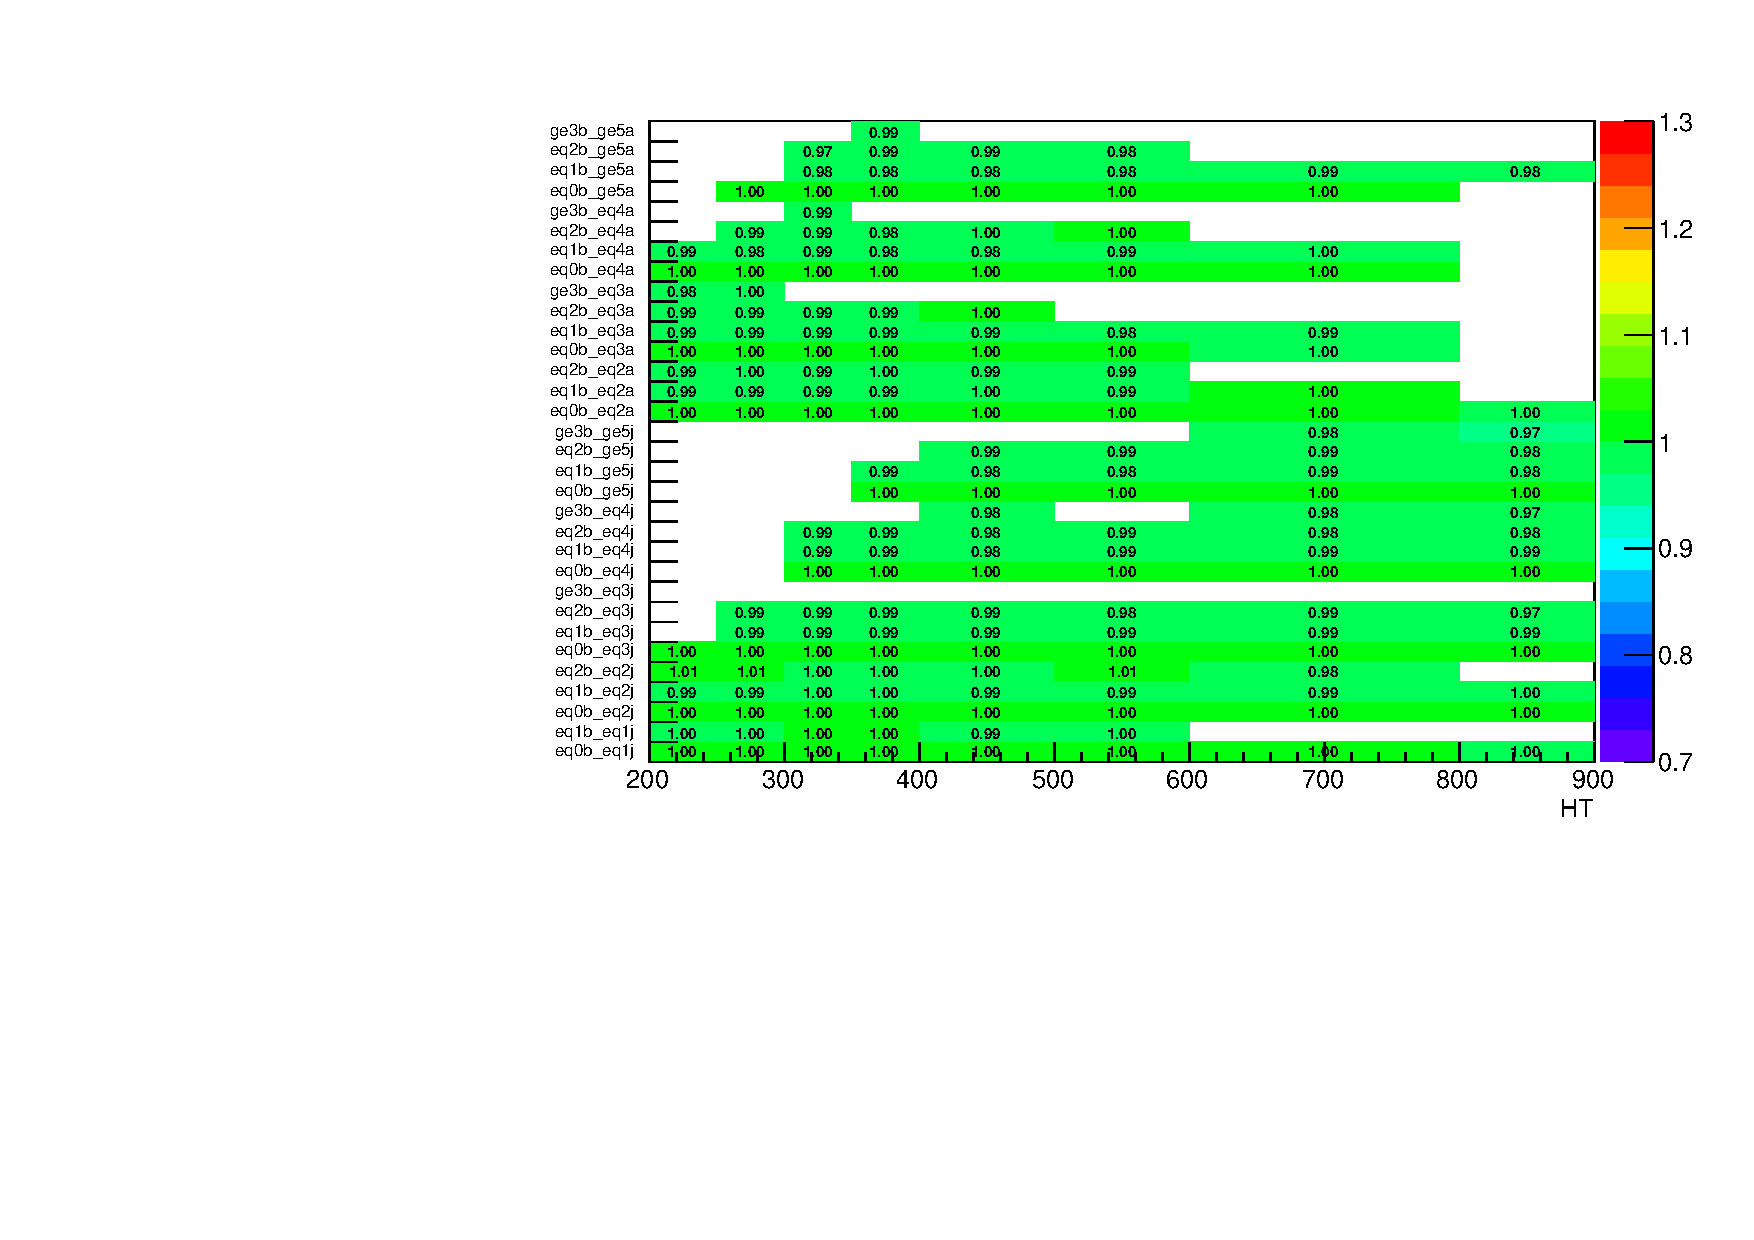
\includegraphics[width=0.4\textwidth]{Figures/backgroundPrediction/mcSystematics12p9fb/Zinv/mu/ratiotfh_ht_mht_allbsfLightWeight_Down.pdf}
%   }\\
%
%   \caption{\label{fig:tfSyst_bsfl_muToZinv} The relative change in the
%   $\mj \rightarrow (\znunu)$ transfer
%   factors when varying b tag SF for light jets in MC within its uncertainties, as a function of \scalht and jet category. 
%   Variations corresponding to $+1\sigma$ ($-1\sigma$) are shown in the left (right) figure. 
%   }
% \end{figure}
%
% \begin{figure}[!h]
%   \centering
%   \subfloat[b tag SF (light) up variation]{
%     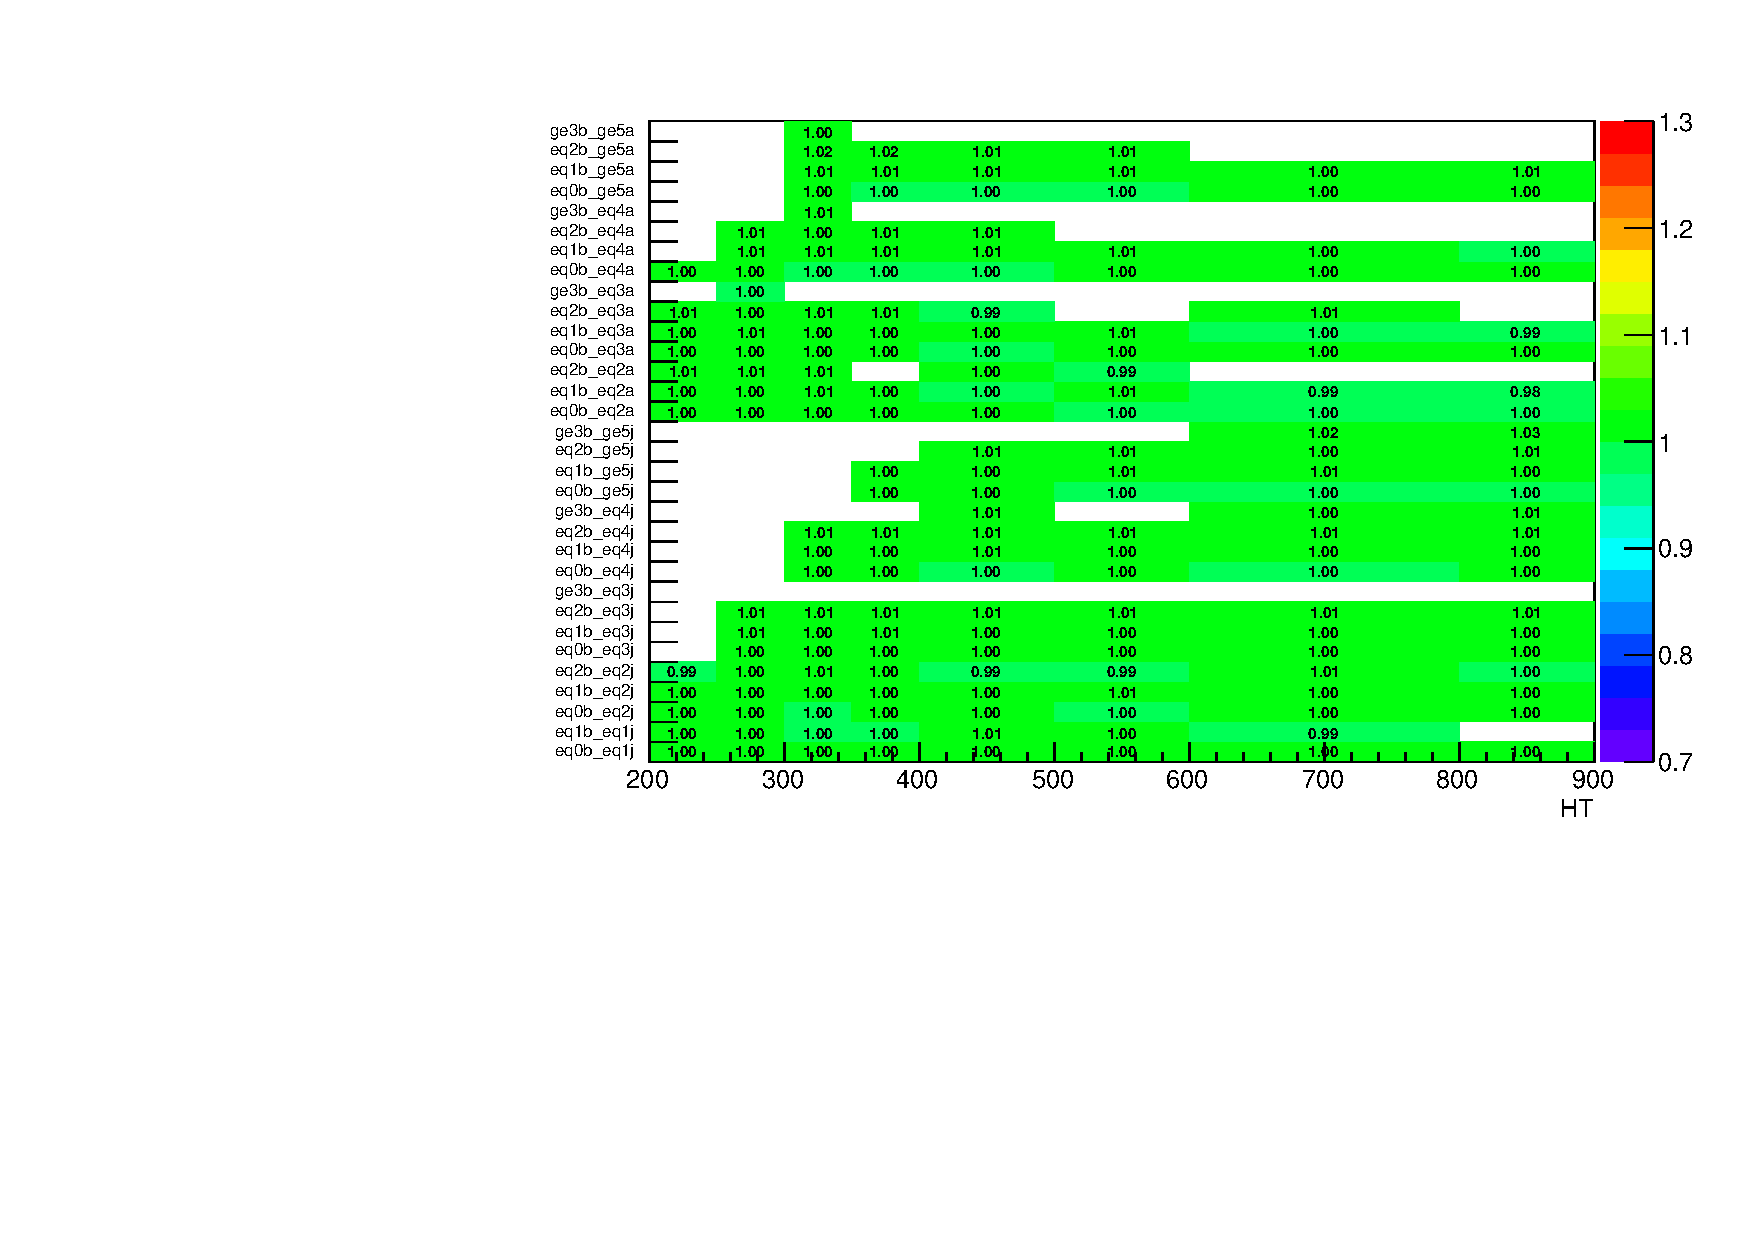
\includegraphics[width=0.4\textwidth]{Figures/backgroundPrediction/mcSystematics12p9fb/Zinv/mumu/ratiotfh_ht_mht_allbsfLightWeight_Up.pdf}
%   } ~~
%   \subfloat[b tag SF (light) down variation]{
%     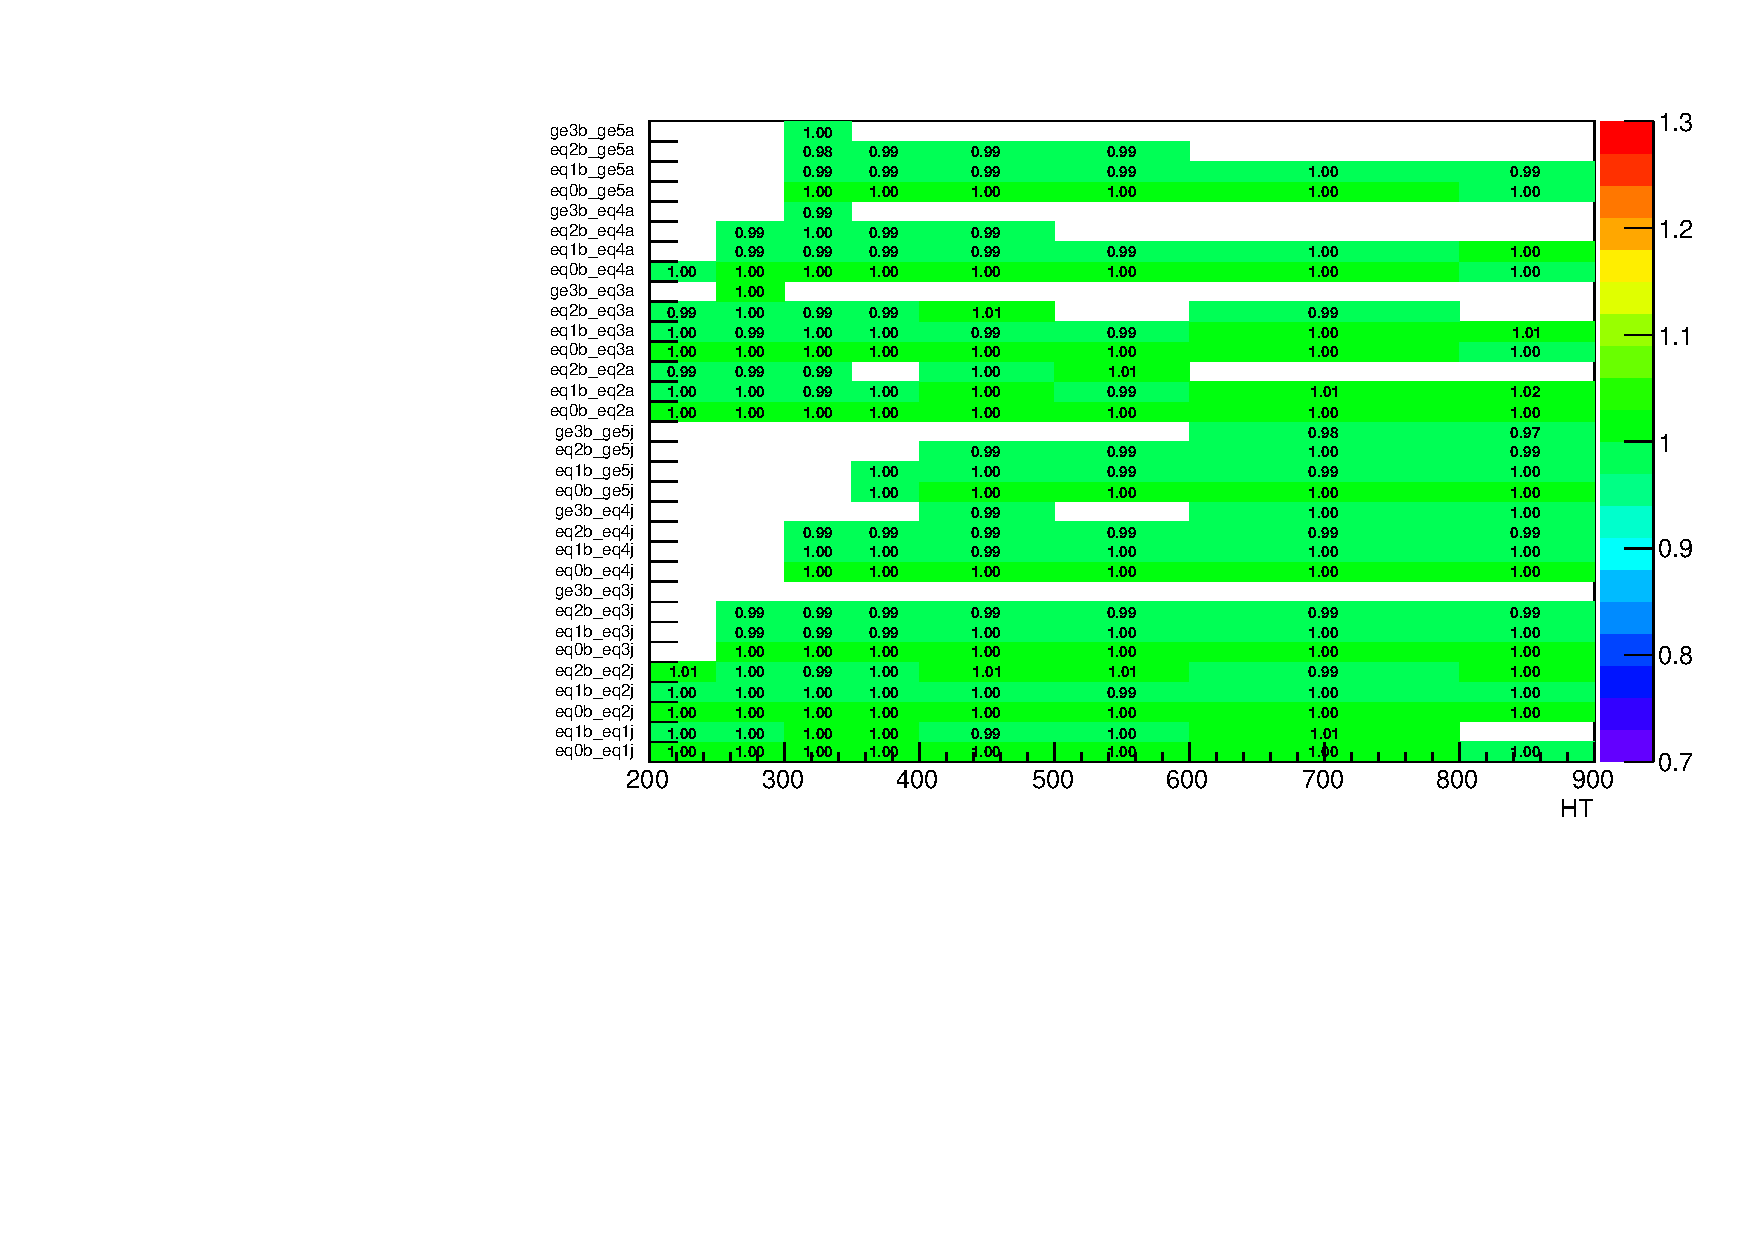
\includegraphics[width=0.4\textwidth]{Figures/backgroundPrediction/mcSystematics12p9fb/Zinv/mumu/ratiotfh_ht_mht_allbsfLightWeight_Down.pdf}
%   }\\
%
%   \caption{\label{fig:tfSyst_bsfl_mumuToZinv} The relative change in
%   the $\mmj \rightarrow (\znunu)$ transfer
%   factors when varying b tag SF for light jets in MC within its uncertainties, as a function of \scalht and jet category. 
%   Variations corresponding to $+1\sigma$ ($-1\sigma$) are shown in the left (right) figure. 
%   }
% \end{figure}
%
% \begin{figure}[!h]
%   \centering
%   \subfloat[b tag SF (light) up variation]{
%     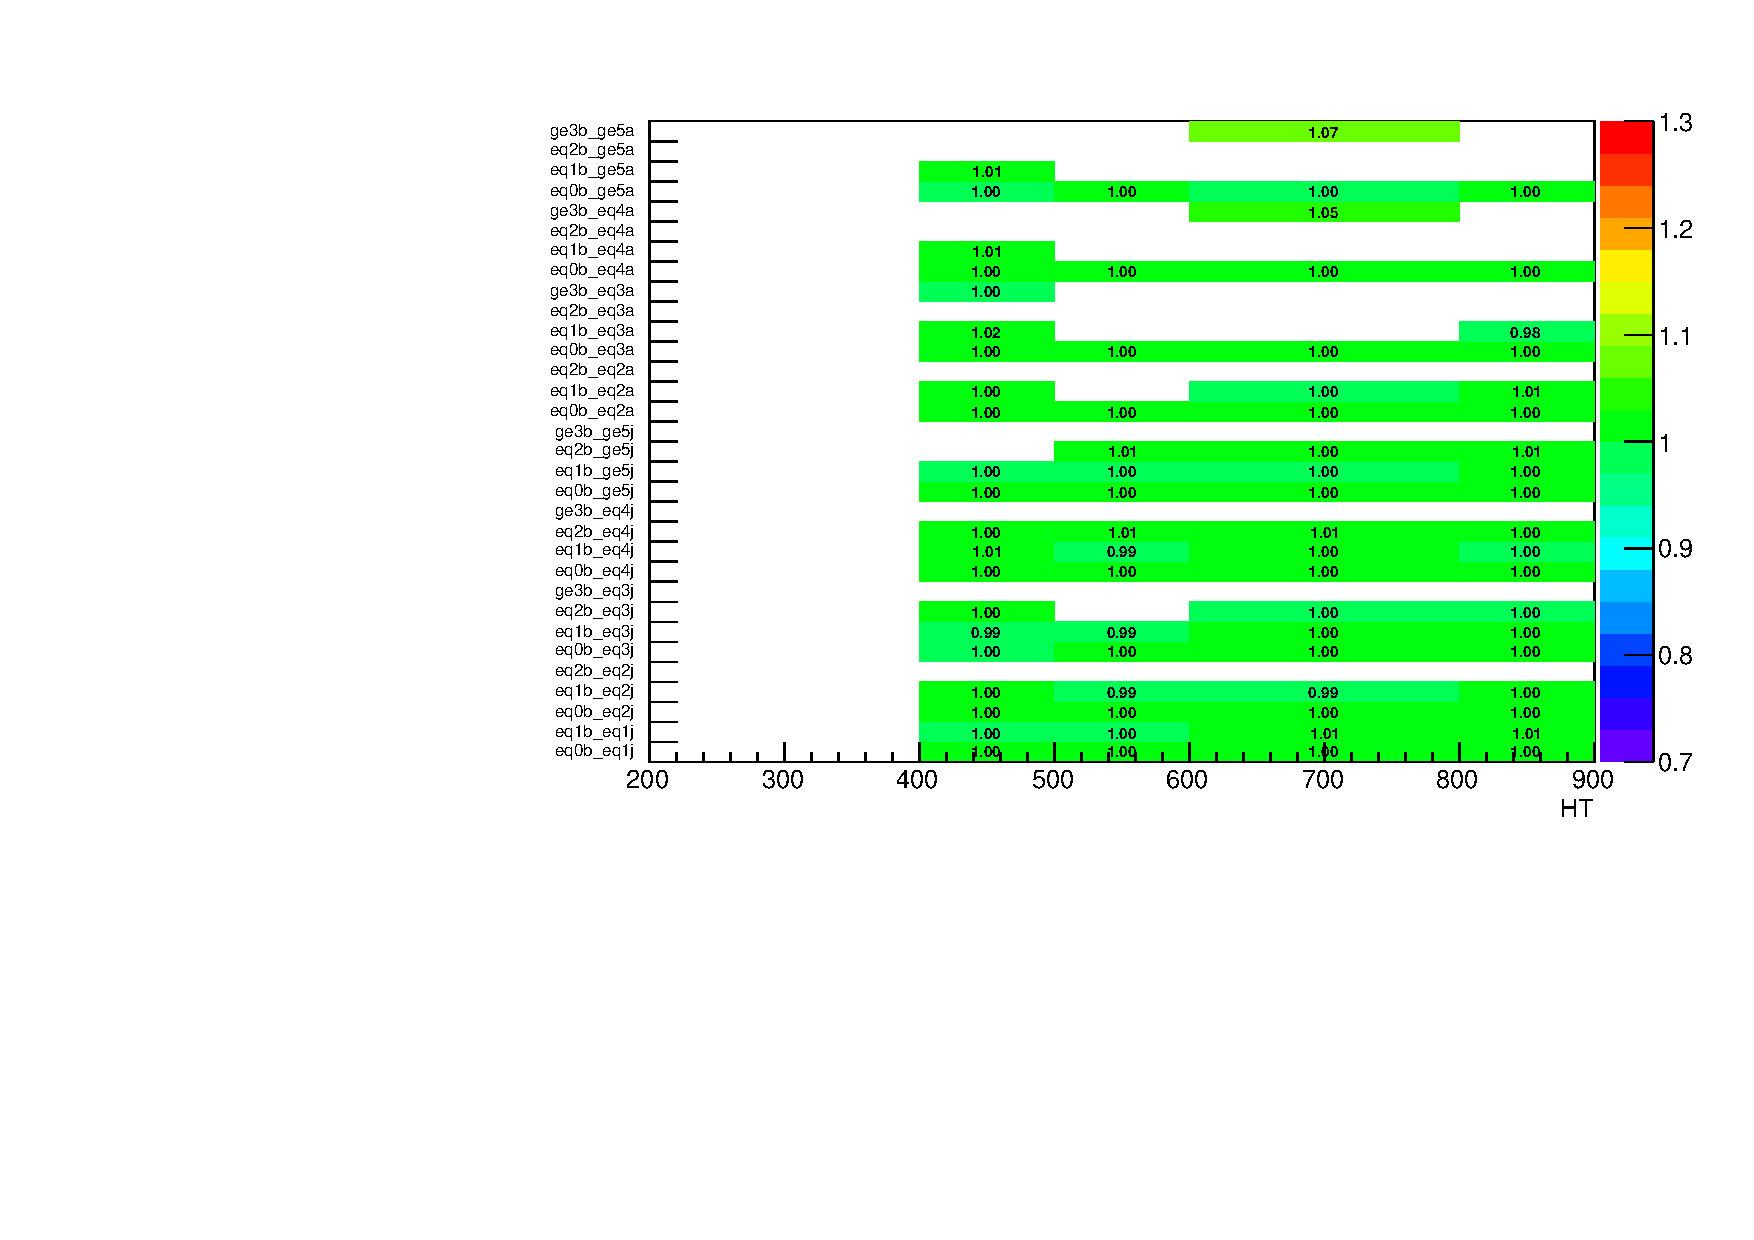
\includegraphics[width=0.4\textwidth]{Figures/backgroundPrediction/mcSystematics12p9fb/Zinv/gj/ratiotfh_ht_mht_allbsfLightWeight_Up.pdf}
%   } ~~
%   \subfloat[b tag SF (light) down variation]{
%     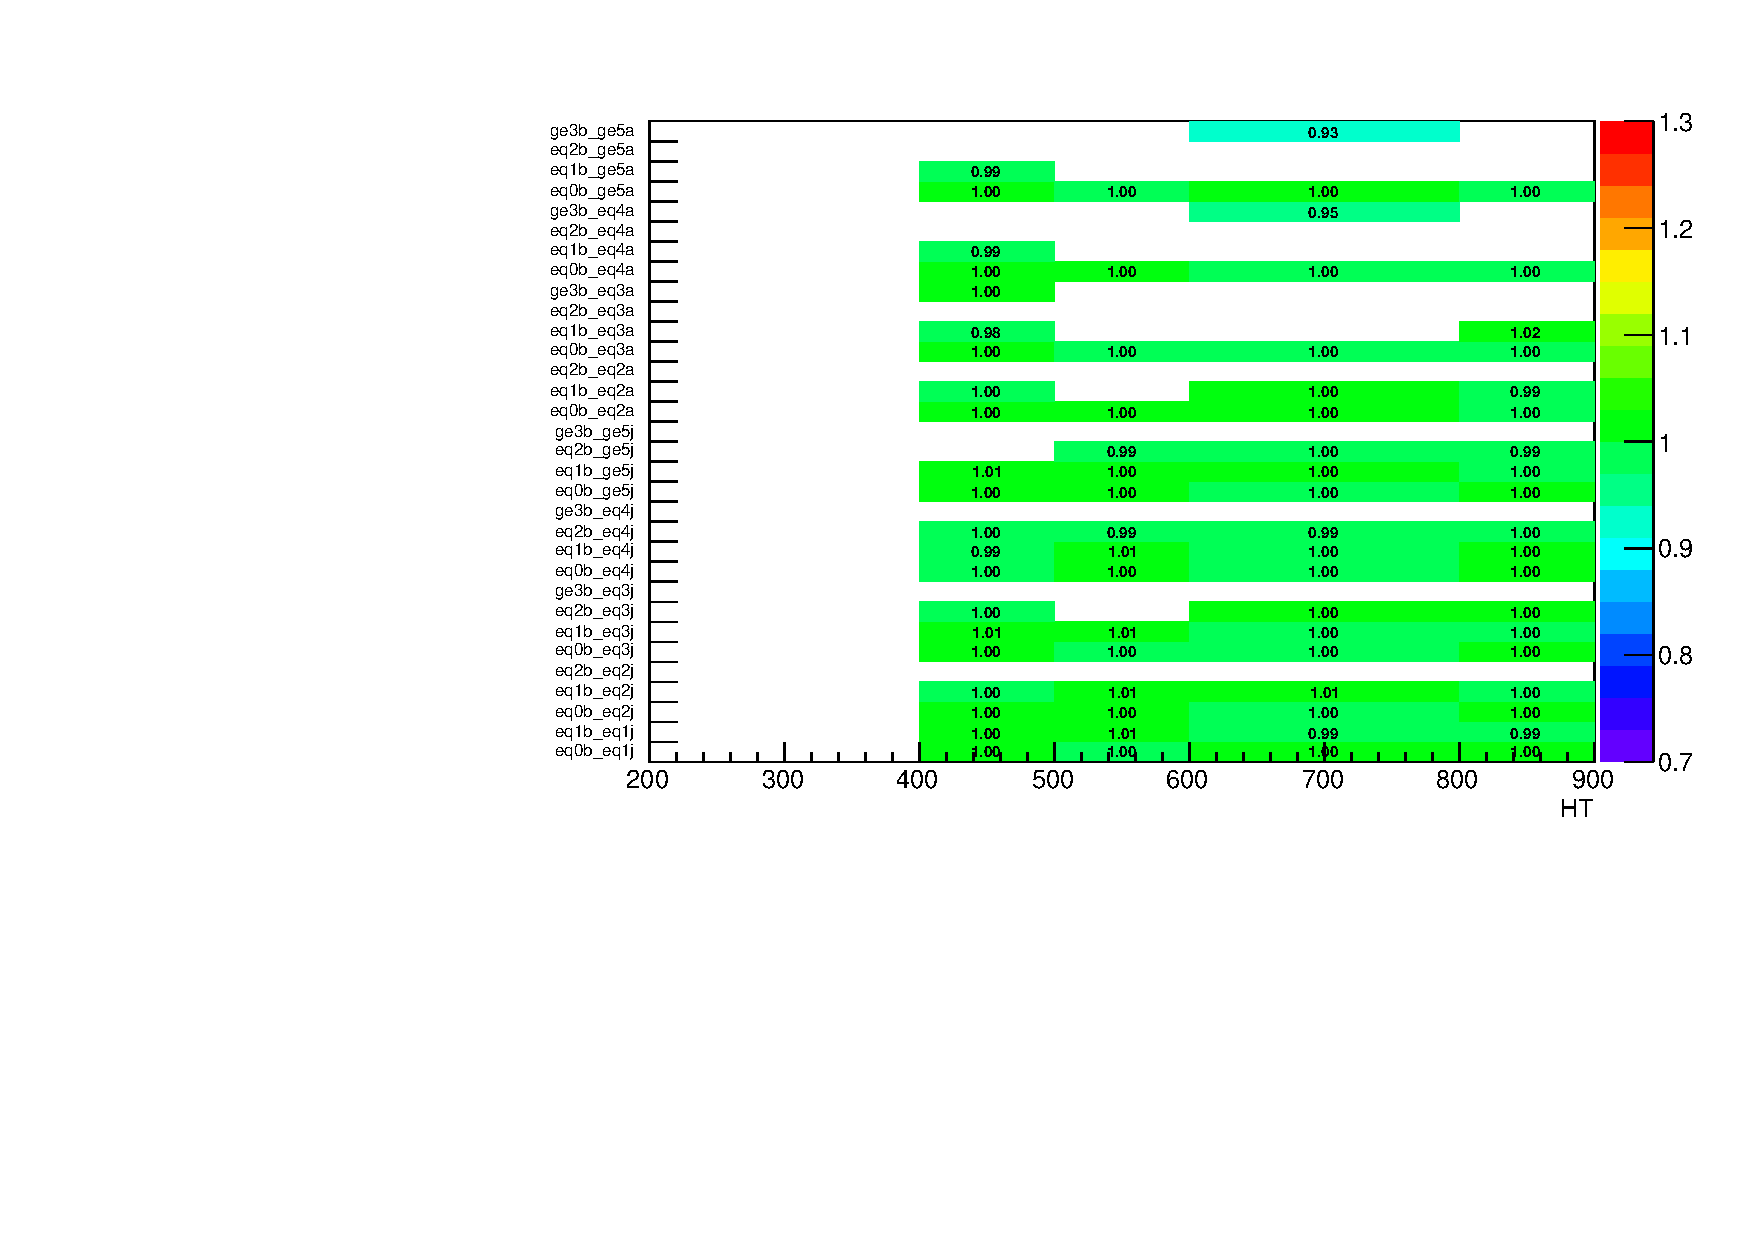
\includegraphics[width=0.4\textwidth]{Figures/backgroundPrediction/mcSystematics12p9fb/Zinv/gj/ratiotfh_ht_mht_allbsfLightWeight_Down.pdf}
%   }\\
%
%   \caption{\label{fig:tfSyst_bsfl_gjToZinv} The relative change in the
%   $\gj \rightarrow (\znunu)$ transfer
%   factors when varying b tag SF for light jets in MC within its uncertainties, as a function of \scalht and jet category. 
%   Variations corresponding to $+1\sigma$ ($-1\sigma$) are shown in the left (right) figure. 
%   }
% \end{figure}
%
% \begin{figure}[!h]
%   \centering
%   \subfloat[b tag SF (light) up variation]{
%     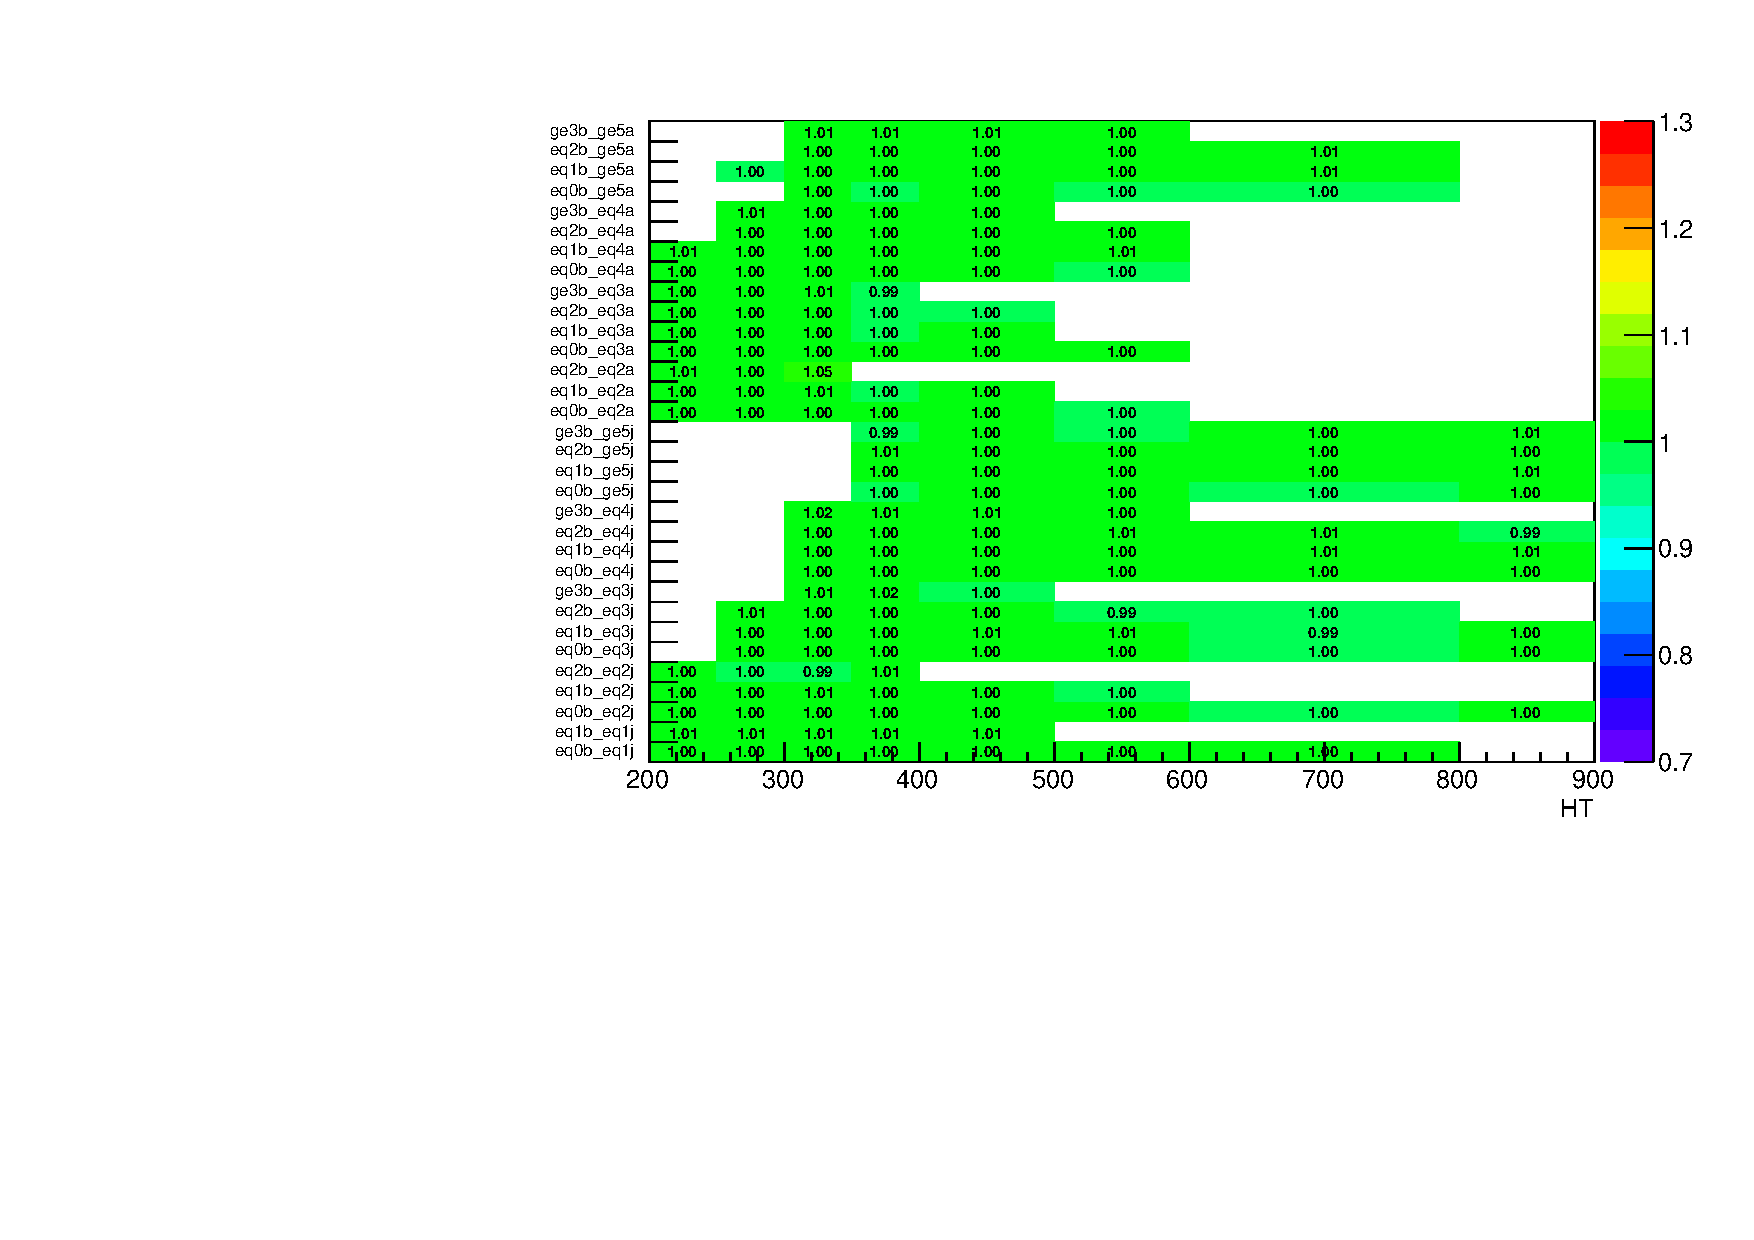
\includegraphics[width=0.4\textwidth]{Figures/backgroundPrediction/mcSystematics12p9fb/Ttw/mu/ratiotfh_ht_mht_allbsfLightWeight_Up.pdf}
%   } ~~
%   \subfloat[b tag SF (light) down variation]{
%     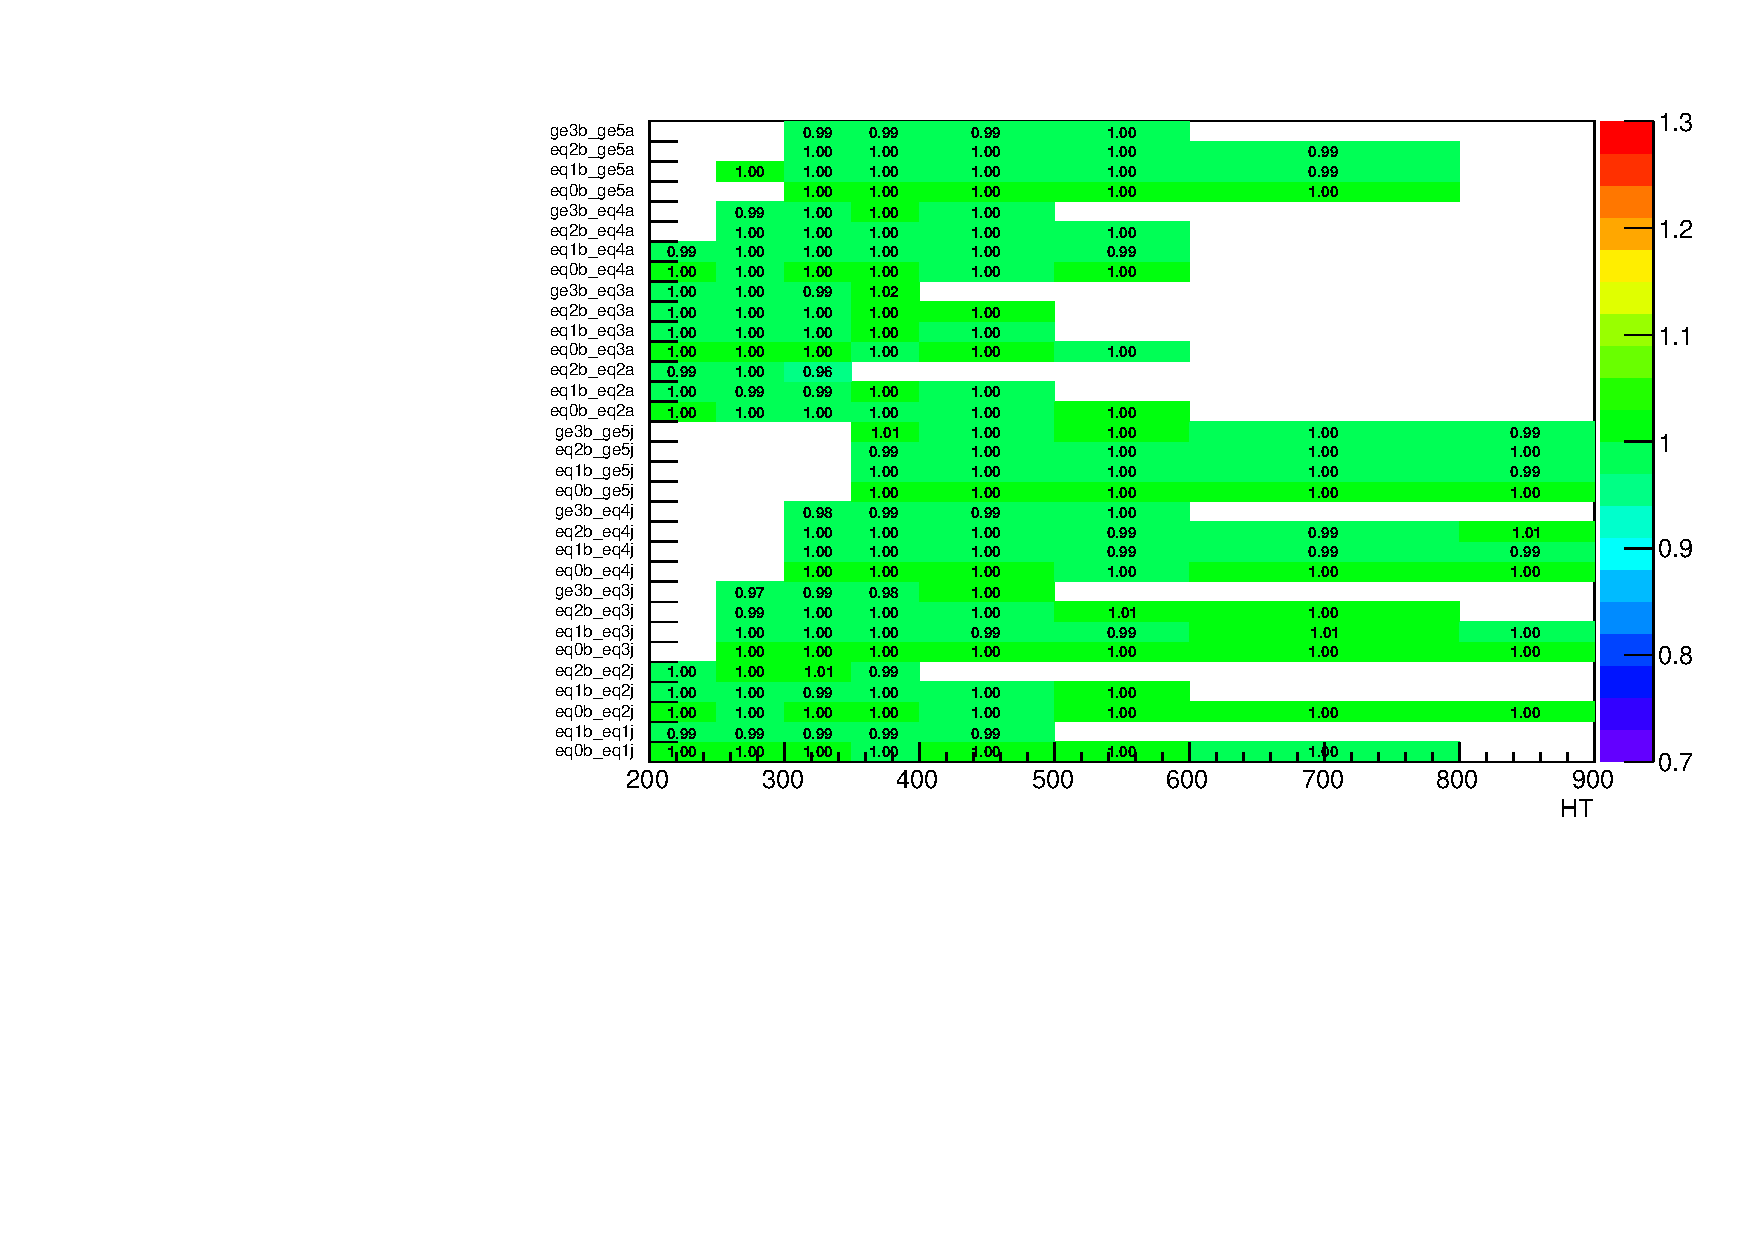
\includegraphics[width=0.4\textwidth]{Figures/backgroundPrediction/mcSystematics12p9fb/Ttw/mu/ratiotfh_ht_mht_allbsfLightWeight_Down.pdf}
%   }\\
%
%   \caption{\label{fig:tfSyst_bsfl_muToTtw} The relative change in the $\mj \rightarrow \mathrm{tt+W}$ transfer
%   factors when varying b tag SF for light jets in MC within its uncertainties, as a function of \scalht and jet category. 
%   Variations corresponding to $+1\sigma$ ($-1\sigma$) are shown in the left (right) figure. 
%   }
% \end{figure}
%
% \clearpage
% \section{Lepton and photon trigger/identification/isolation efficiency}
%
% \begin{figure}[!h]
%   \centering
%   \subfloat[muon scale factor up variation]{
%     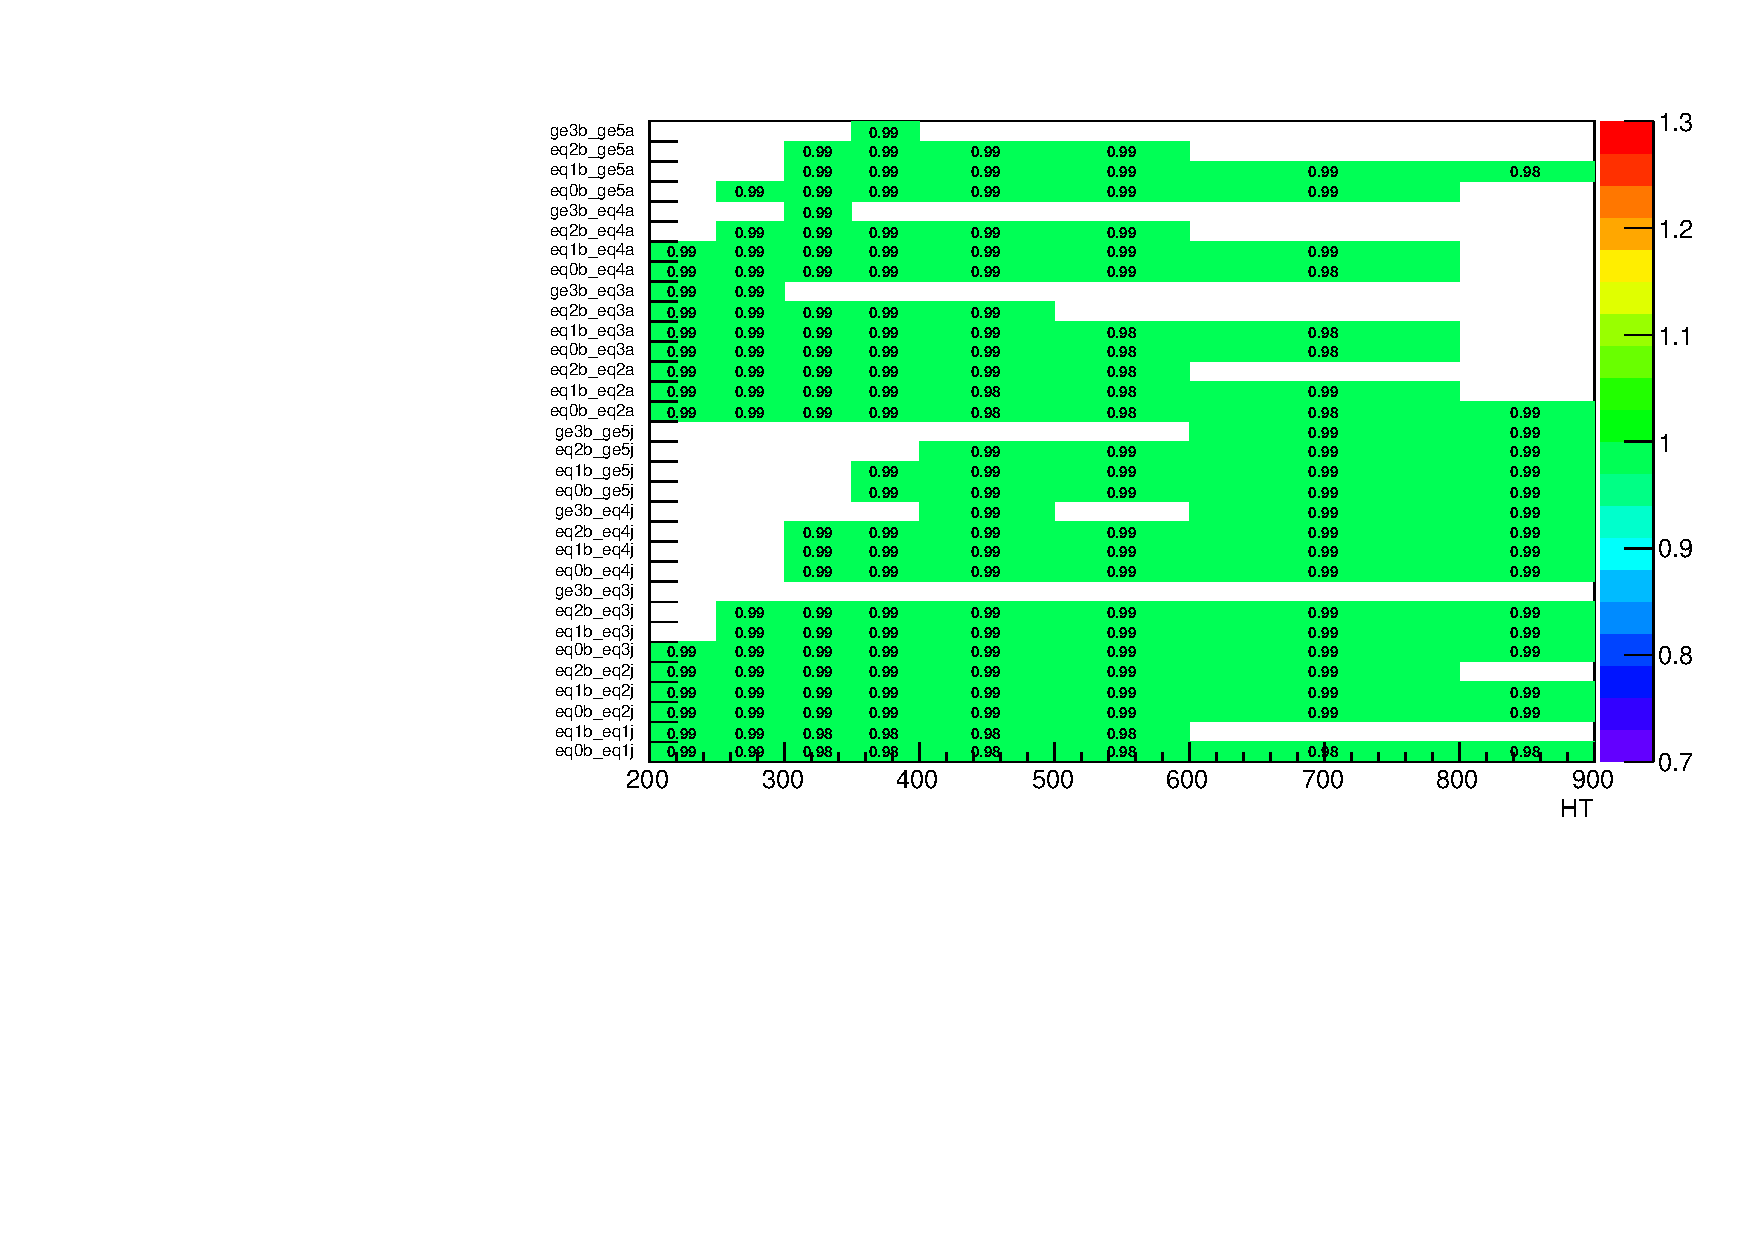
\includegraphics[width=0.4\textwidth]{Figures/backgroundPrediction/mcSystematics12p9fb/Zinv/mu/ratiotfh_ht_mht_allmuonSfWeight_Up.pdf}
%   } ~~
%   \subfloat[muon scale factor down variation]{
%     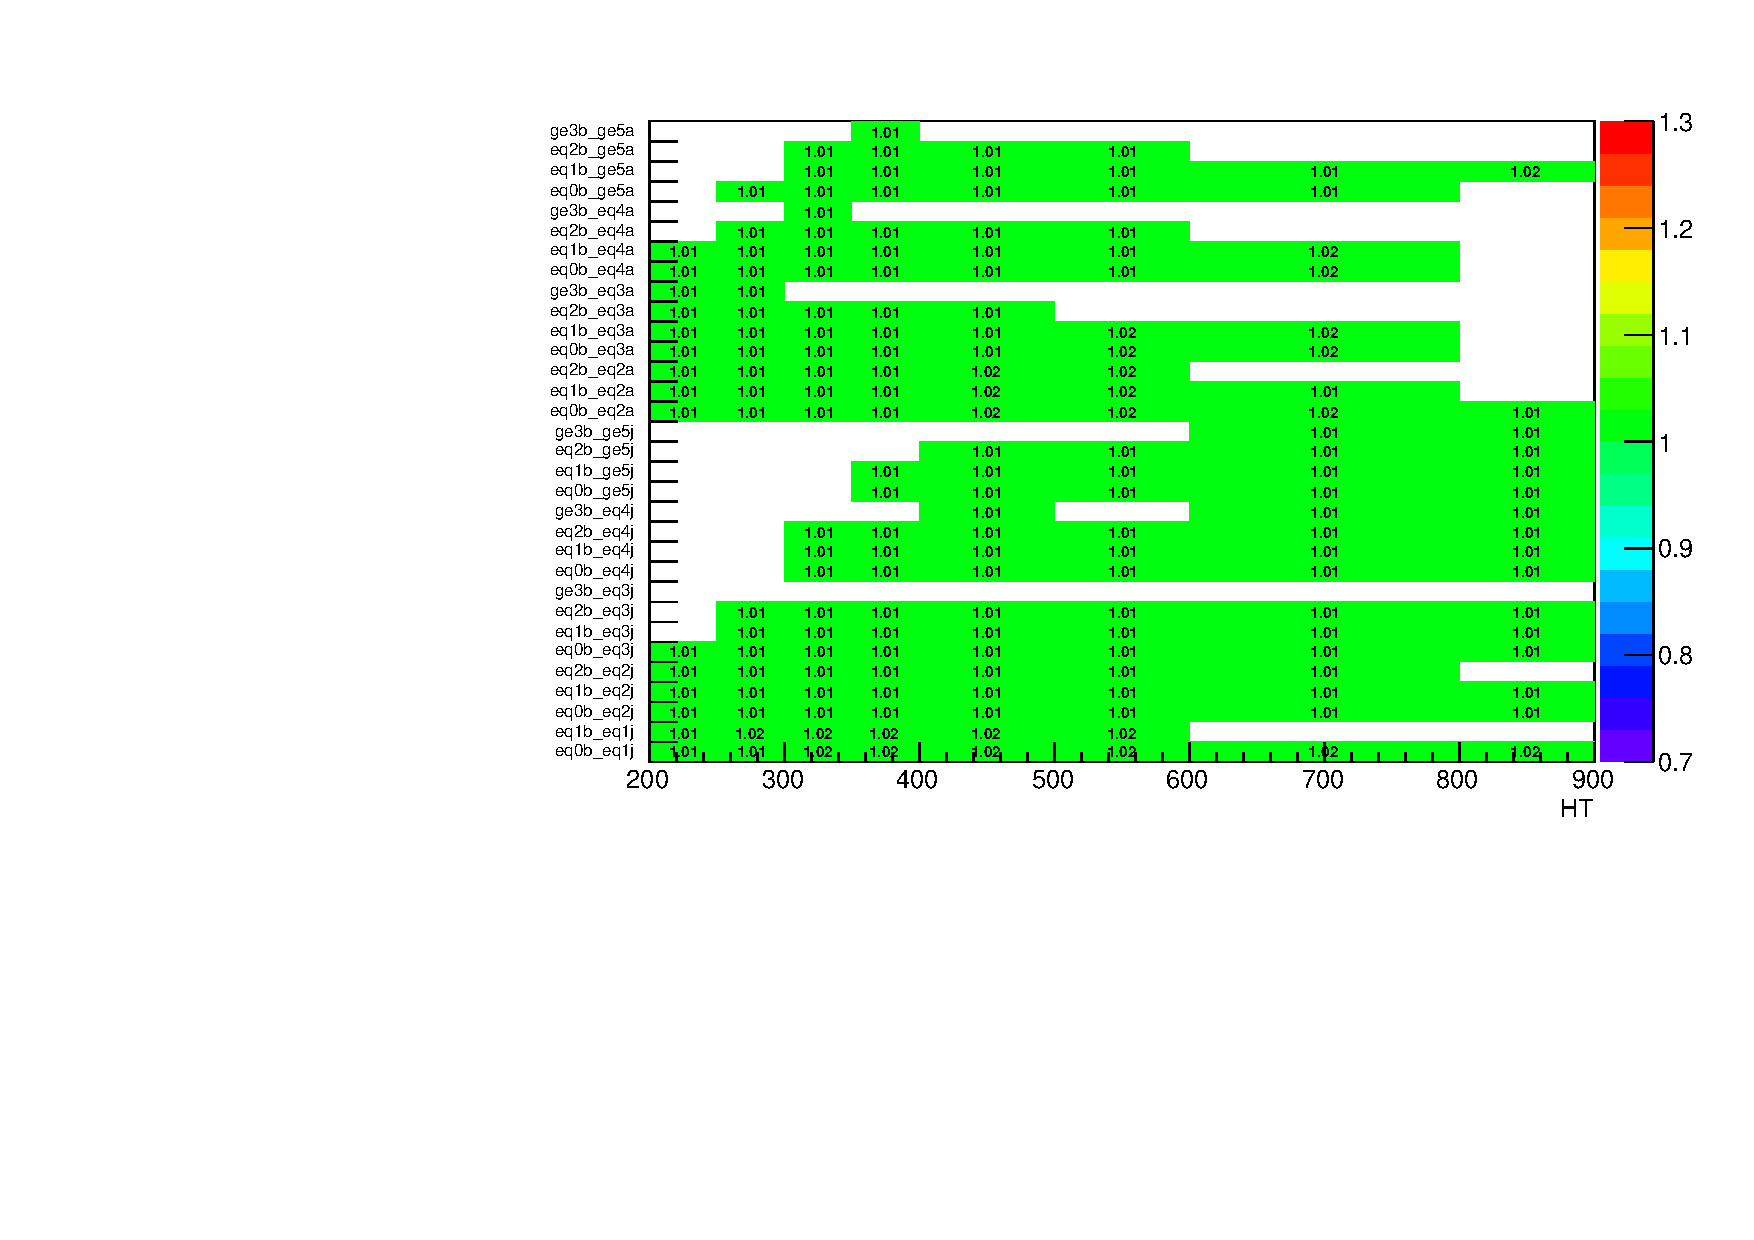
\includegraphics[width=0.4\textwidth]{Figures/backgroundPrediction/mcSystematics12p9fb/Zinv/mu/ratiotfh_ht_mht_allmuonSfWeight_Down.pdf}
%   }\\
%
%   \caption{\label{fig:tfSyst_lepton_muToZinv} The relative change in
%   the $\mj \rightarrow (\znunu)$ transfer
%   factors when varying muon scale factor in MC within its uncertainties, as a function of \scalht and jet category. 
%   Variations corresponding to $+1\sigma$ ($-1\sigma$) are shown in the left (right) figure. 
%   }
% \end{figure}
%
% \begin{figure}[!h]
%   \centering
%   \subfloat[muon scale factor up variation]{
%     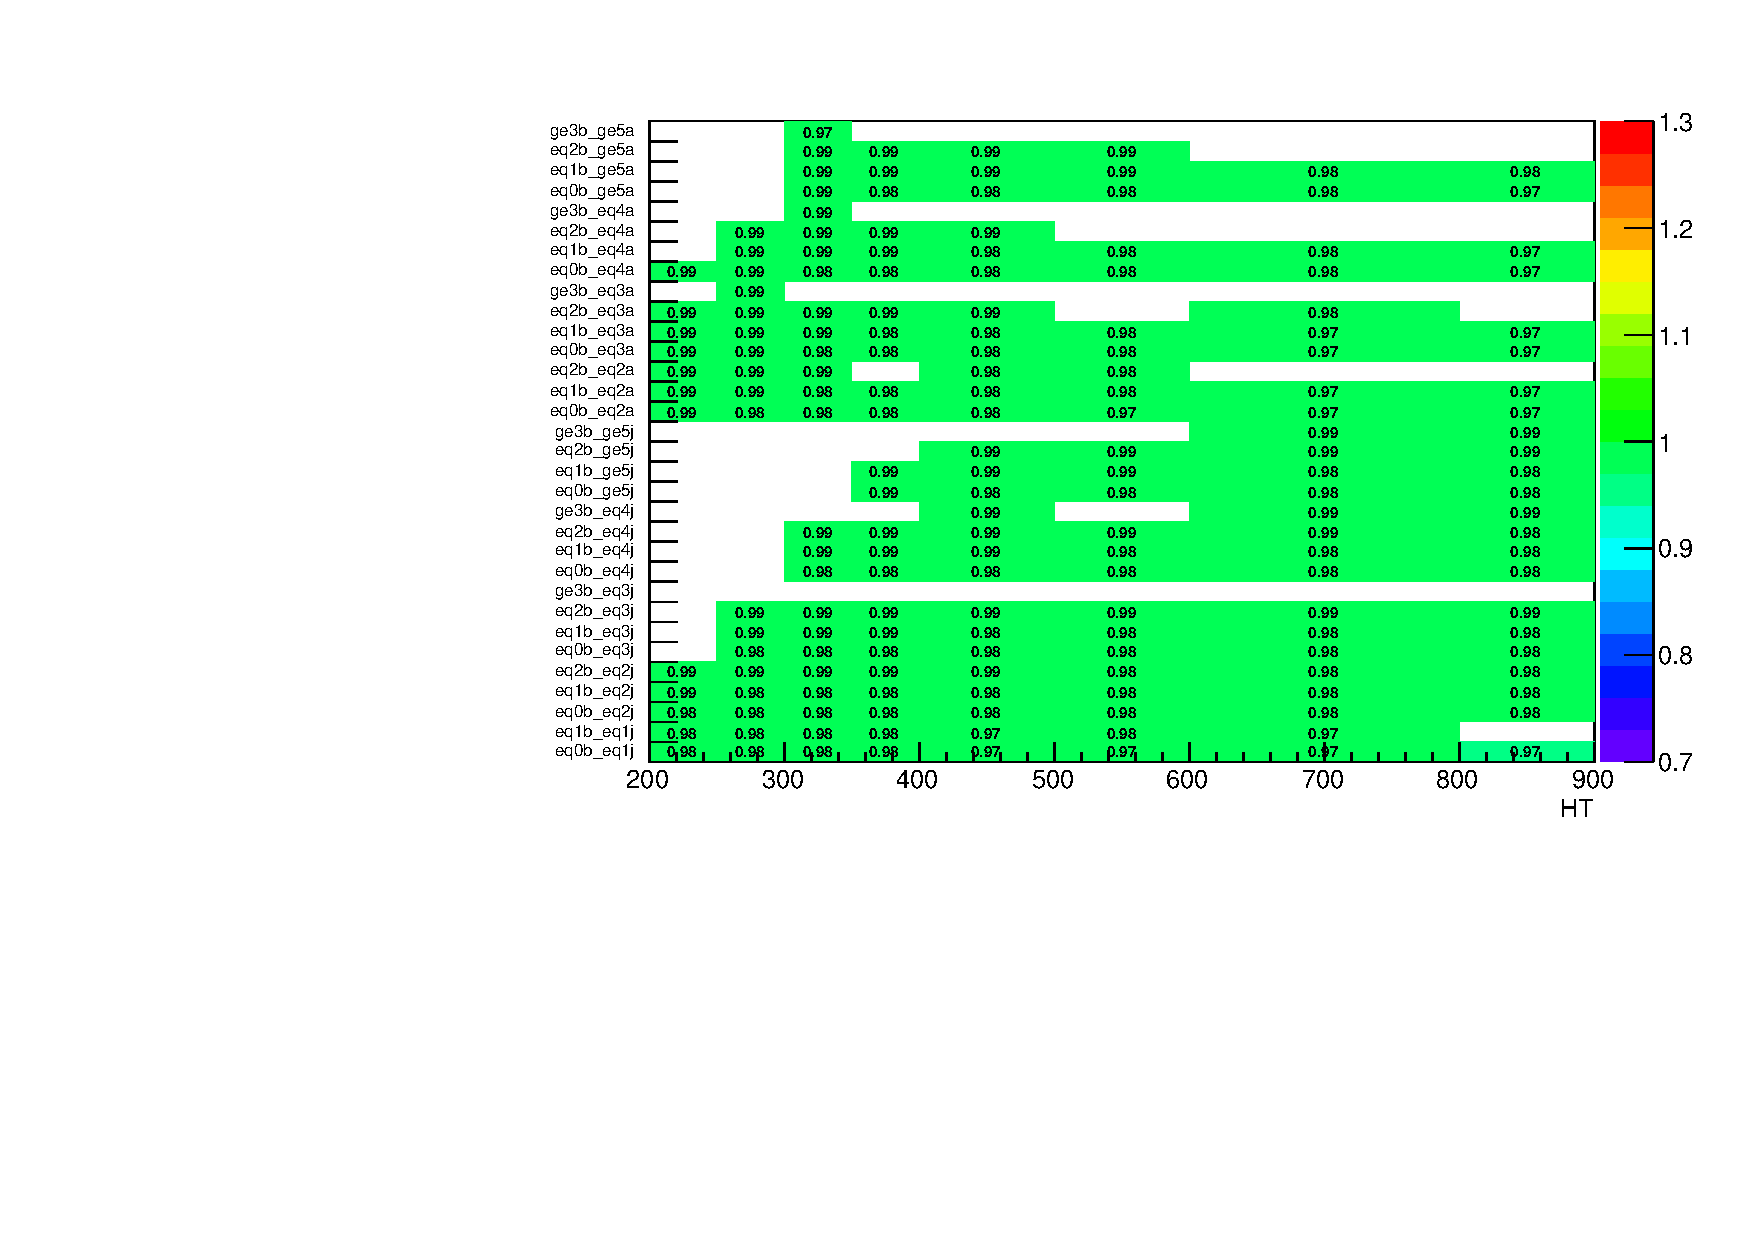
\includegraphics[width=0.4\textwidth]{Figures/backgroundPrediction/mcSystematics12p9fb/Zinv/mumu/ratiotfh_ht_mht_allmuonSfWeight_Up.pdf}
%   } ~~
%   \subfloat[muon scale factor down variation]{
%     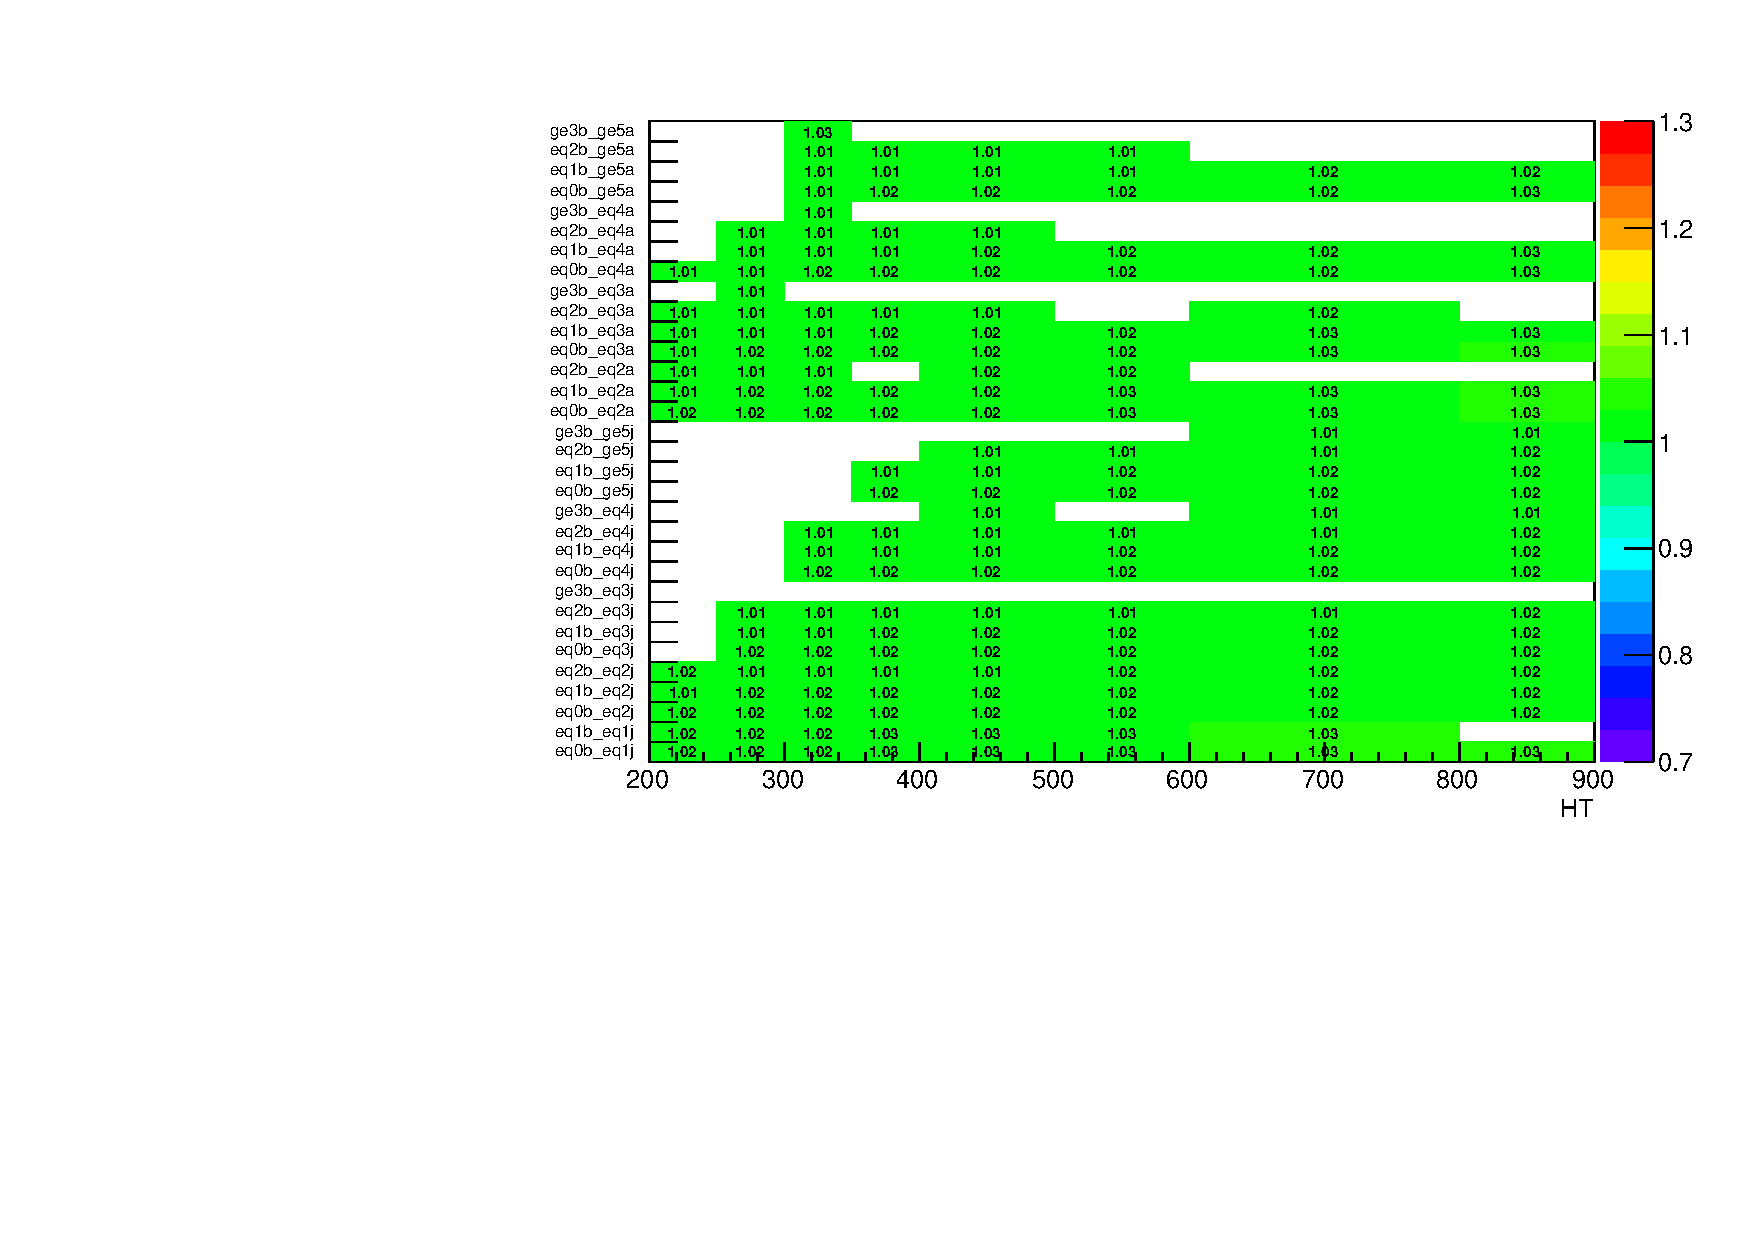
\includegraphics[width=0.4\textwidth]{Figures/backgroundPrediction/mcSystematics12p9fb/Zinv/mumu/ratiotfh_ht_mht_allmuonSfWeight_Down.pdf}
%   }\\
%
%   \caption{\label{fig:tfSyst_lepton_mumuToZinv} The relative change in
%   the $\mmj \rightarrow (\znunu)$ transfer
%   factors when varying muon scale factor in MC within its uncertainties, as a function of \scalht and jet category. 
%   Variations corresponding to $+1\sigma$ ($-1\sigma$) are shown in the left (right) figure. 
%   }
% \end{figure}
%
% \begin{figure}[!h]
%   \centering
%   \subfloat[muon scale factor up variation]{
%     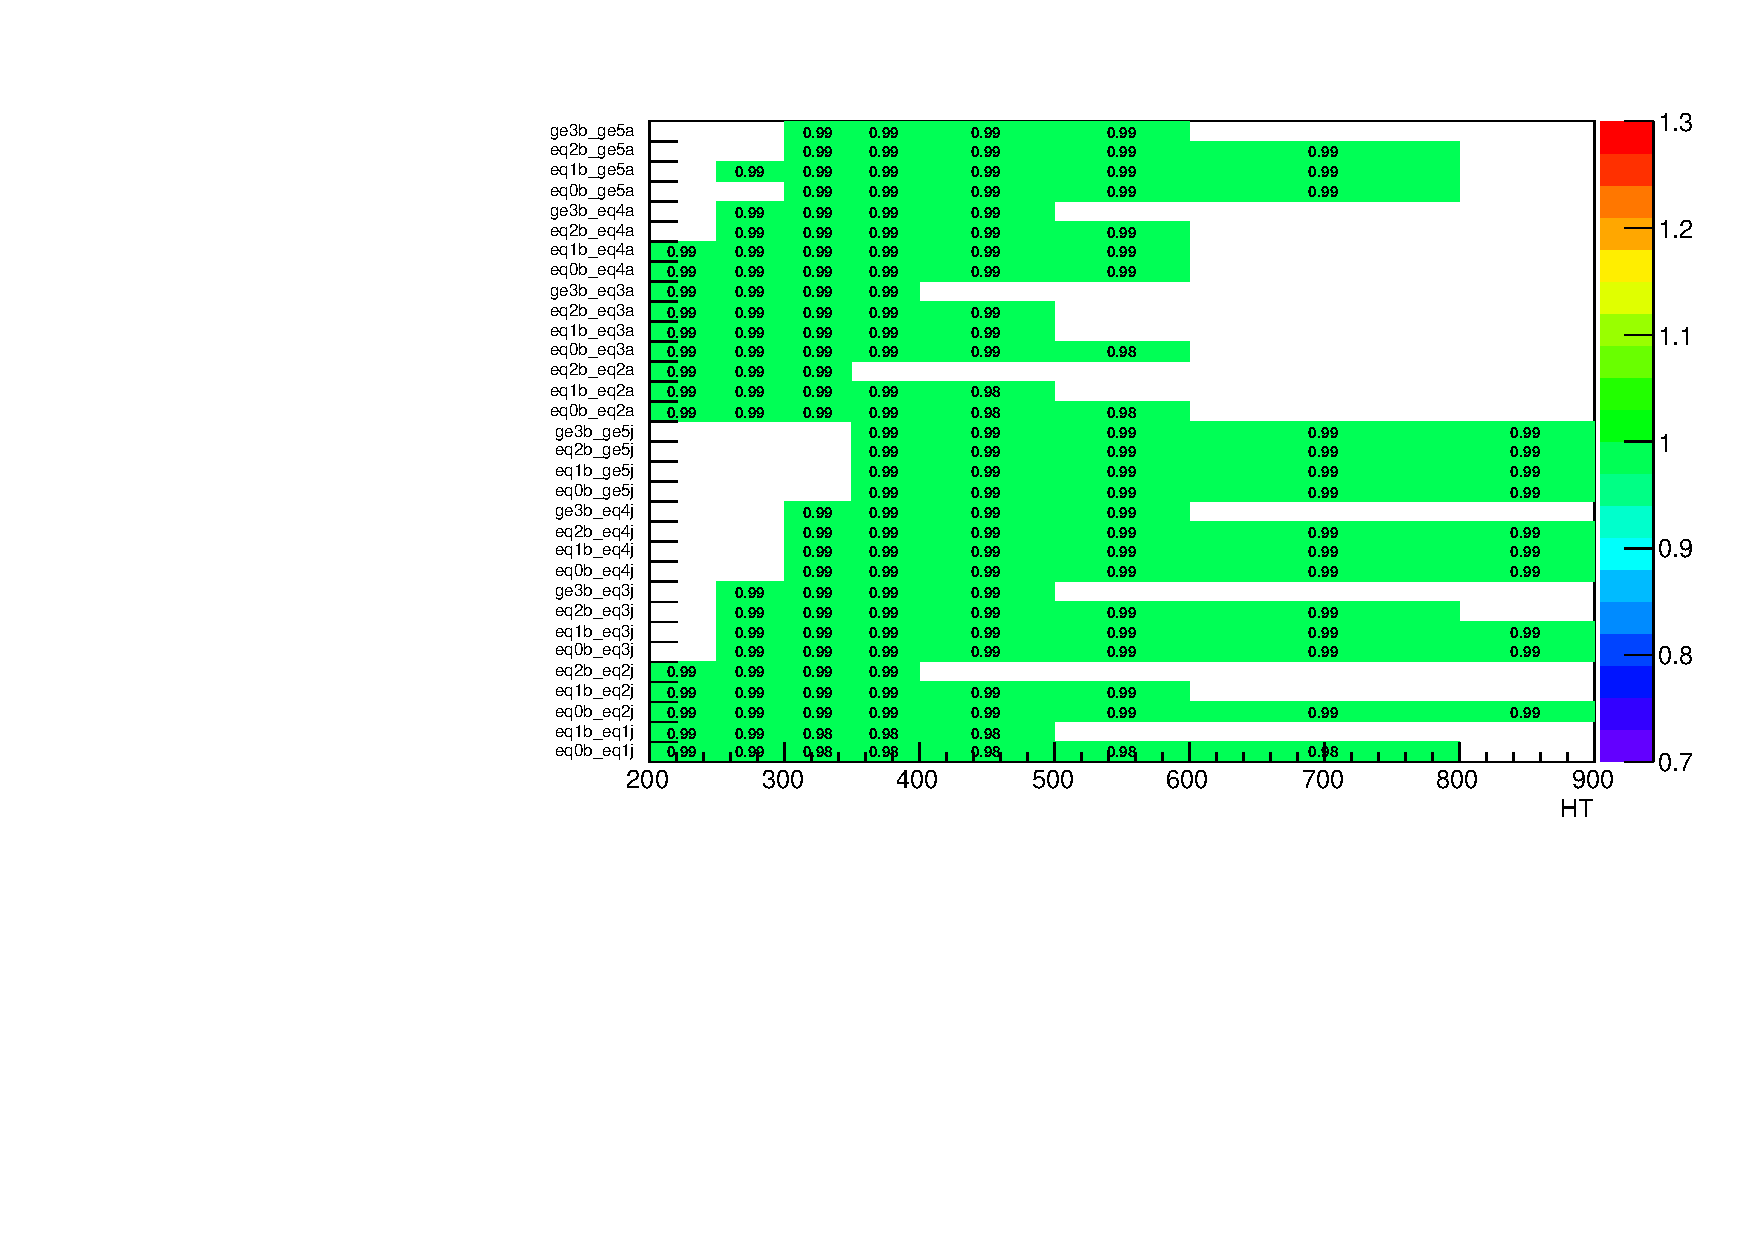
\includegraphics[width=0.4\textwidth]{Figures/backgroundPrediction/mcSystematics12p9fb/Ttw/mu/ratiotfh_ht_mht_allmuonSfWeight_Up.pdf}
%   } ~~
%   \subfloat[muon scale factor down variation]{
%     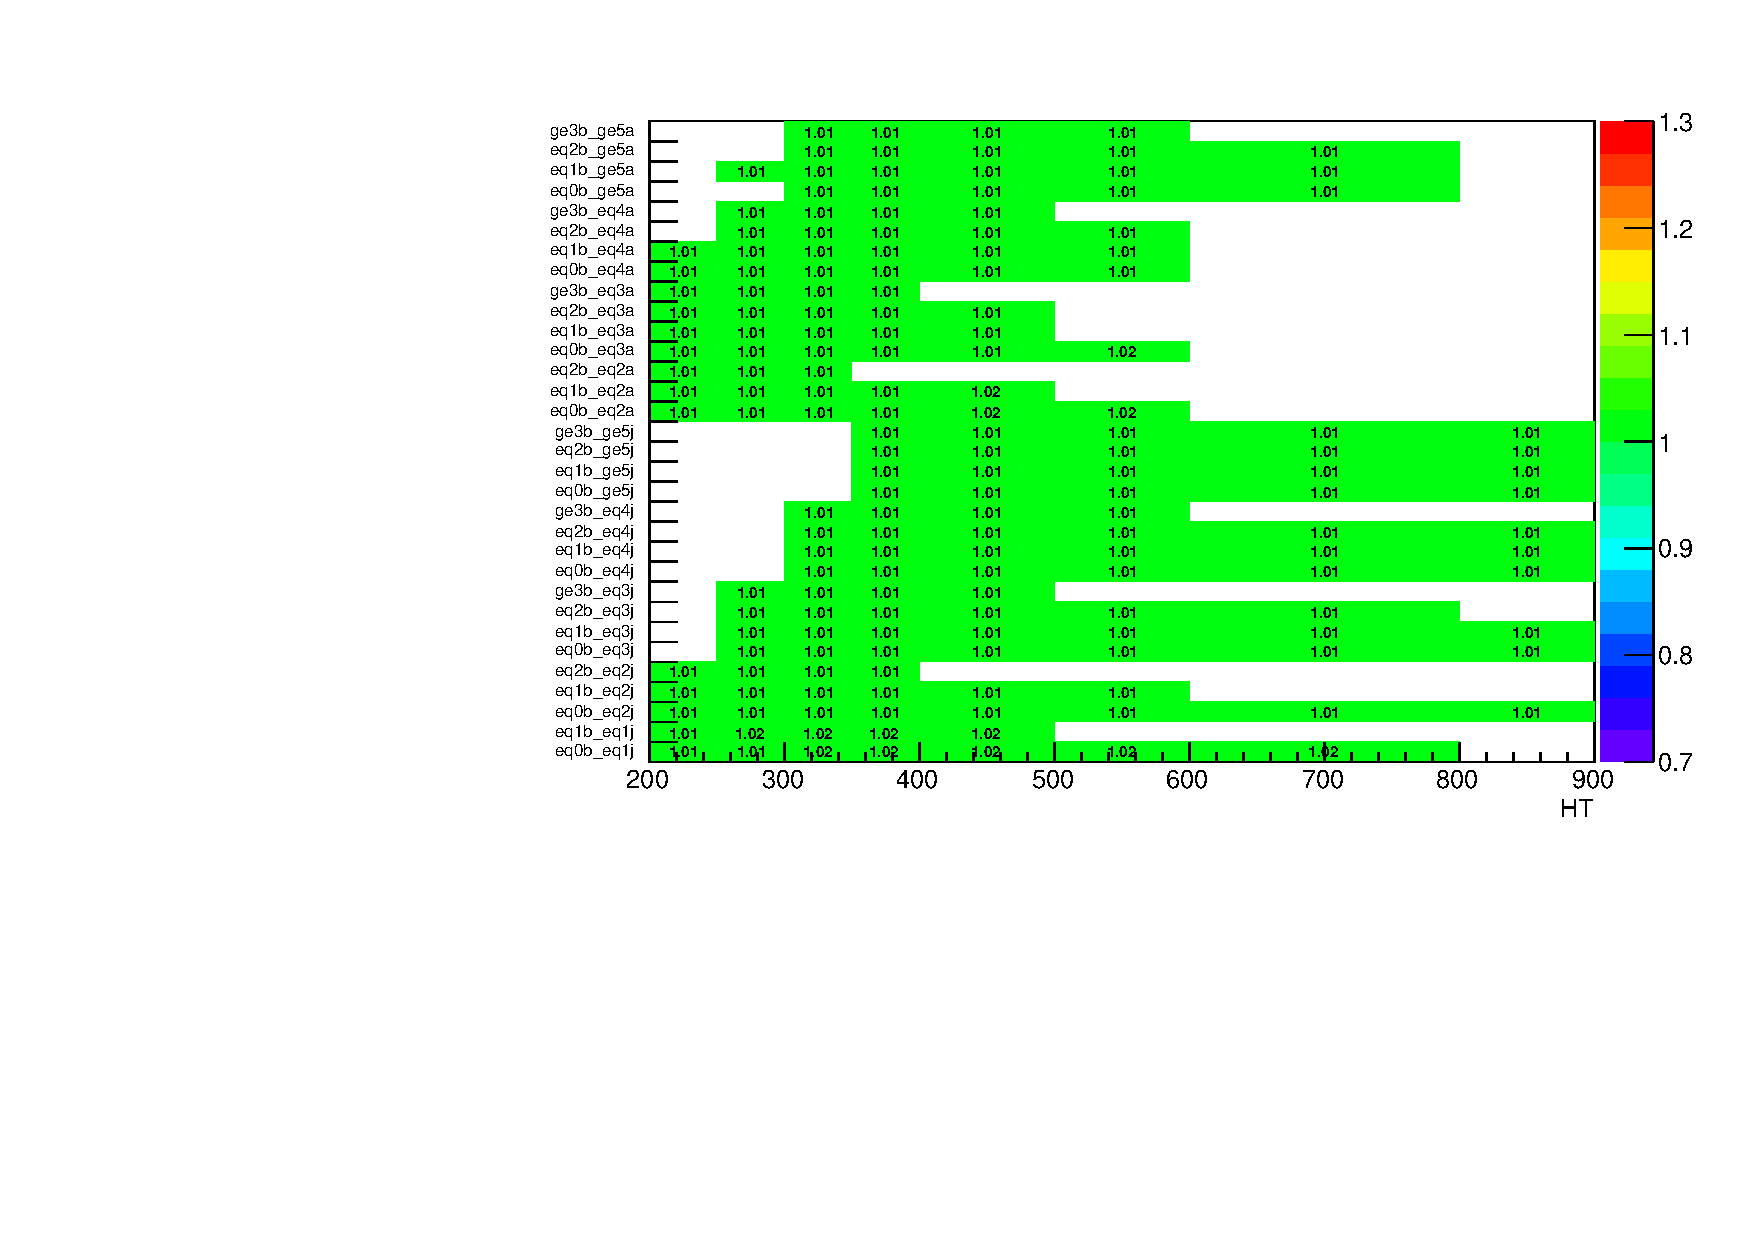
\includegraphics[width=0.4\textwidth]{Figures/backgroundPrediction/mcSystematics12p9fb/Ttw/mu/ratiotfh_ht_mht_allmuonSfWeight_Down.pdf}
%   }\\
%
%   \caption{\label{fig:tfSyst_lepton_muToTtw} The relative change in the $\mj \rightarrow \mathrm{tt+W}$ transfer
%   factors when varying muon scale factor in MC within its uncertainties, as a function of \scalht and jet category. 
%   Variations corresponding to $+1\sigma$ ($-1\sigma$) are shown in the left (right) figure. 
%   }
% \end{figure}
%
% \clearpage
% \section{Photon trigger uncertainty}
%
% \begin{figure}[!h]
%  \centering
%  \subfloat[Photon trigger weight up variation]{
%    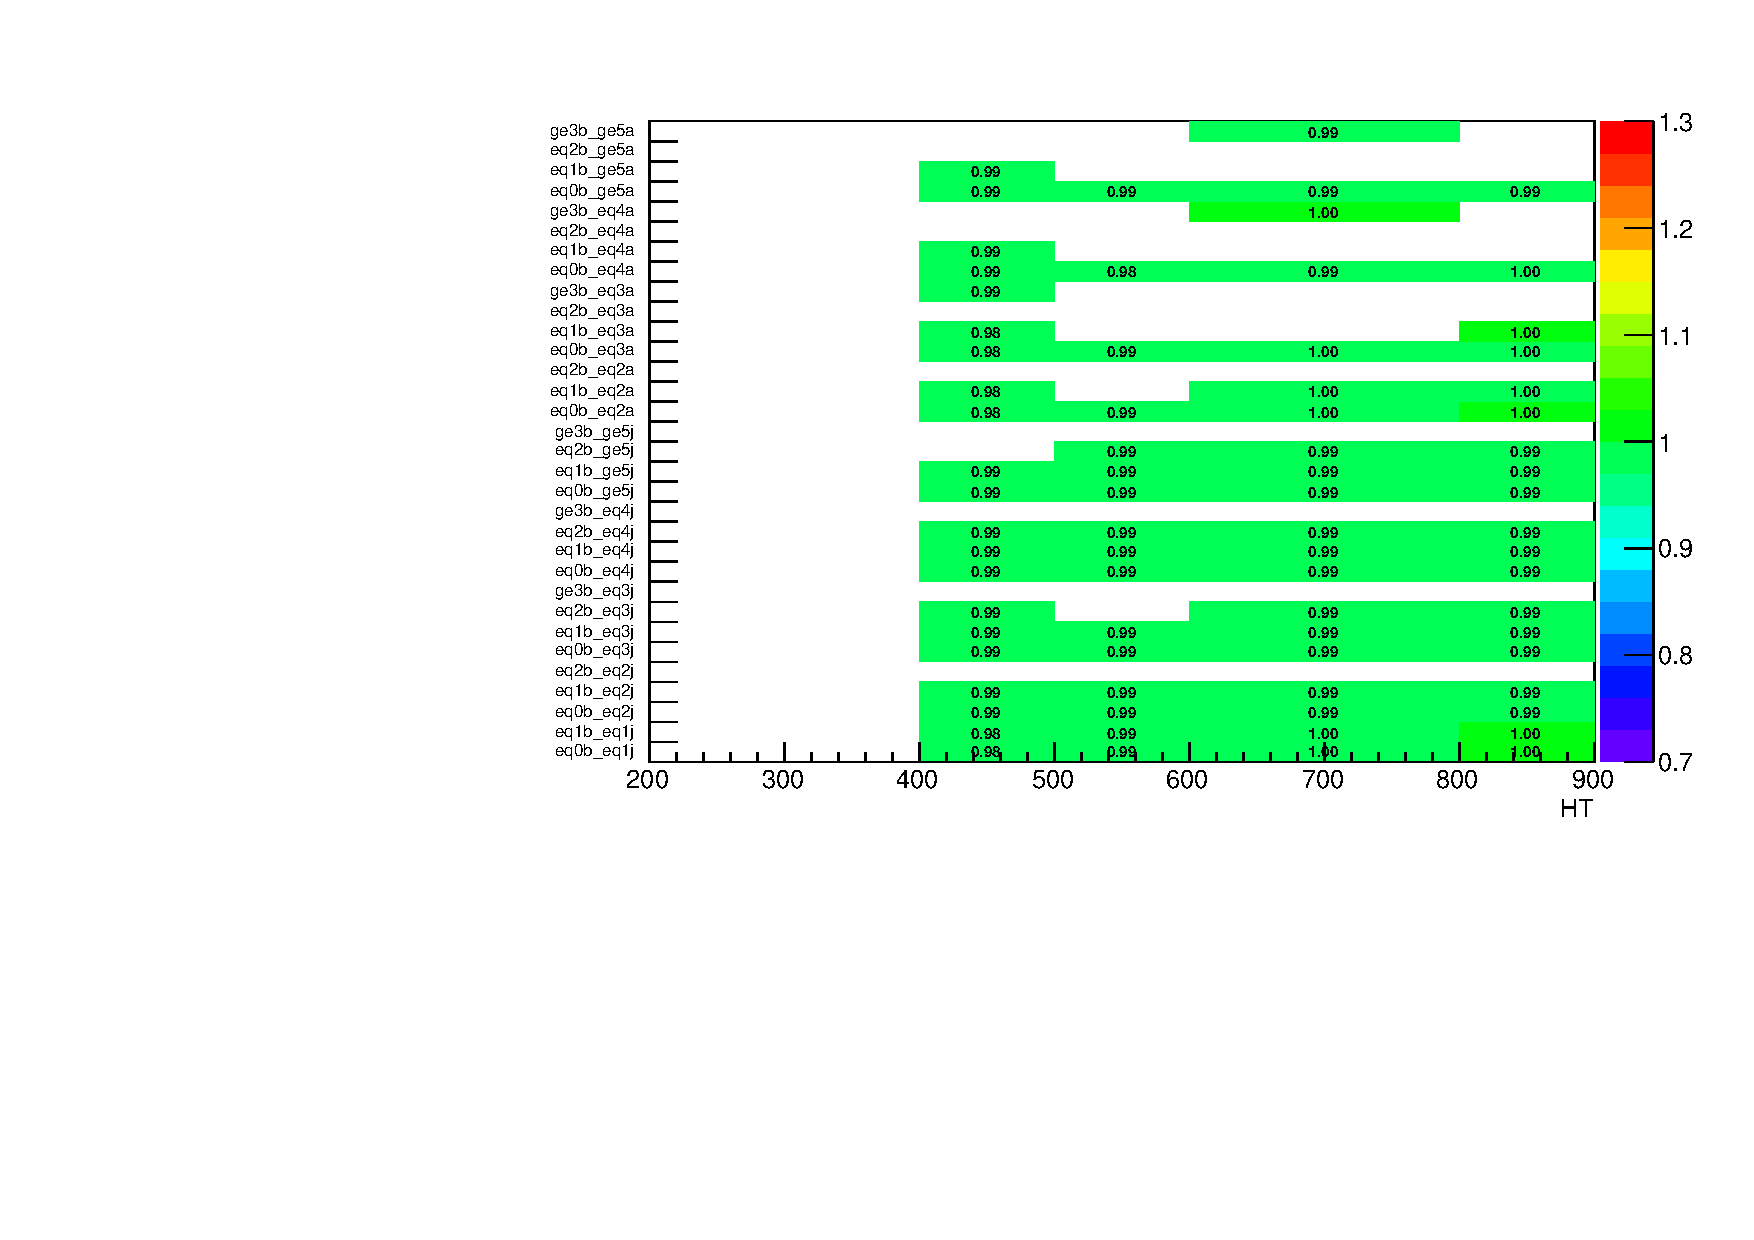
\includegraphics[width=0.4\textwidth]{Figures/backgroundPrediction/mcSystematics12p9fb/Zinv/gj/ratiotfh_ht_mht_allphotonTriggerWeight_Up.pdf}
%  } ~~
%  \subfloat[Photon trigger weight down variation]{
%    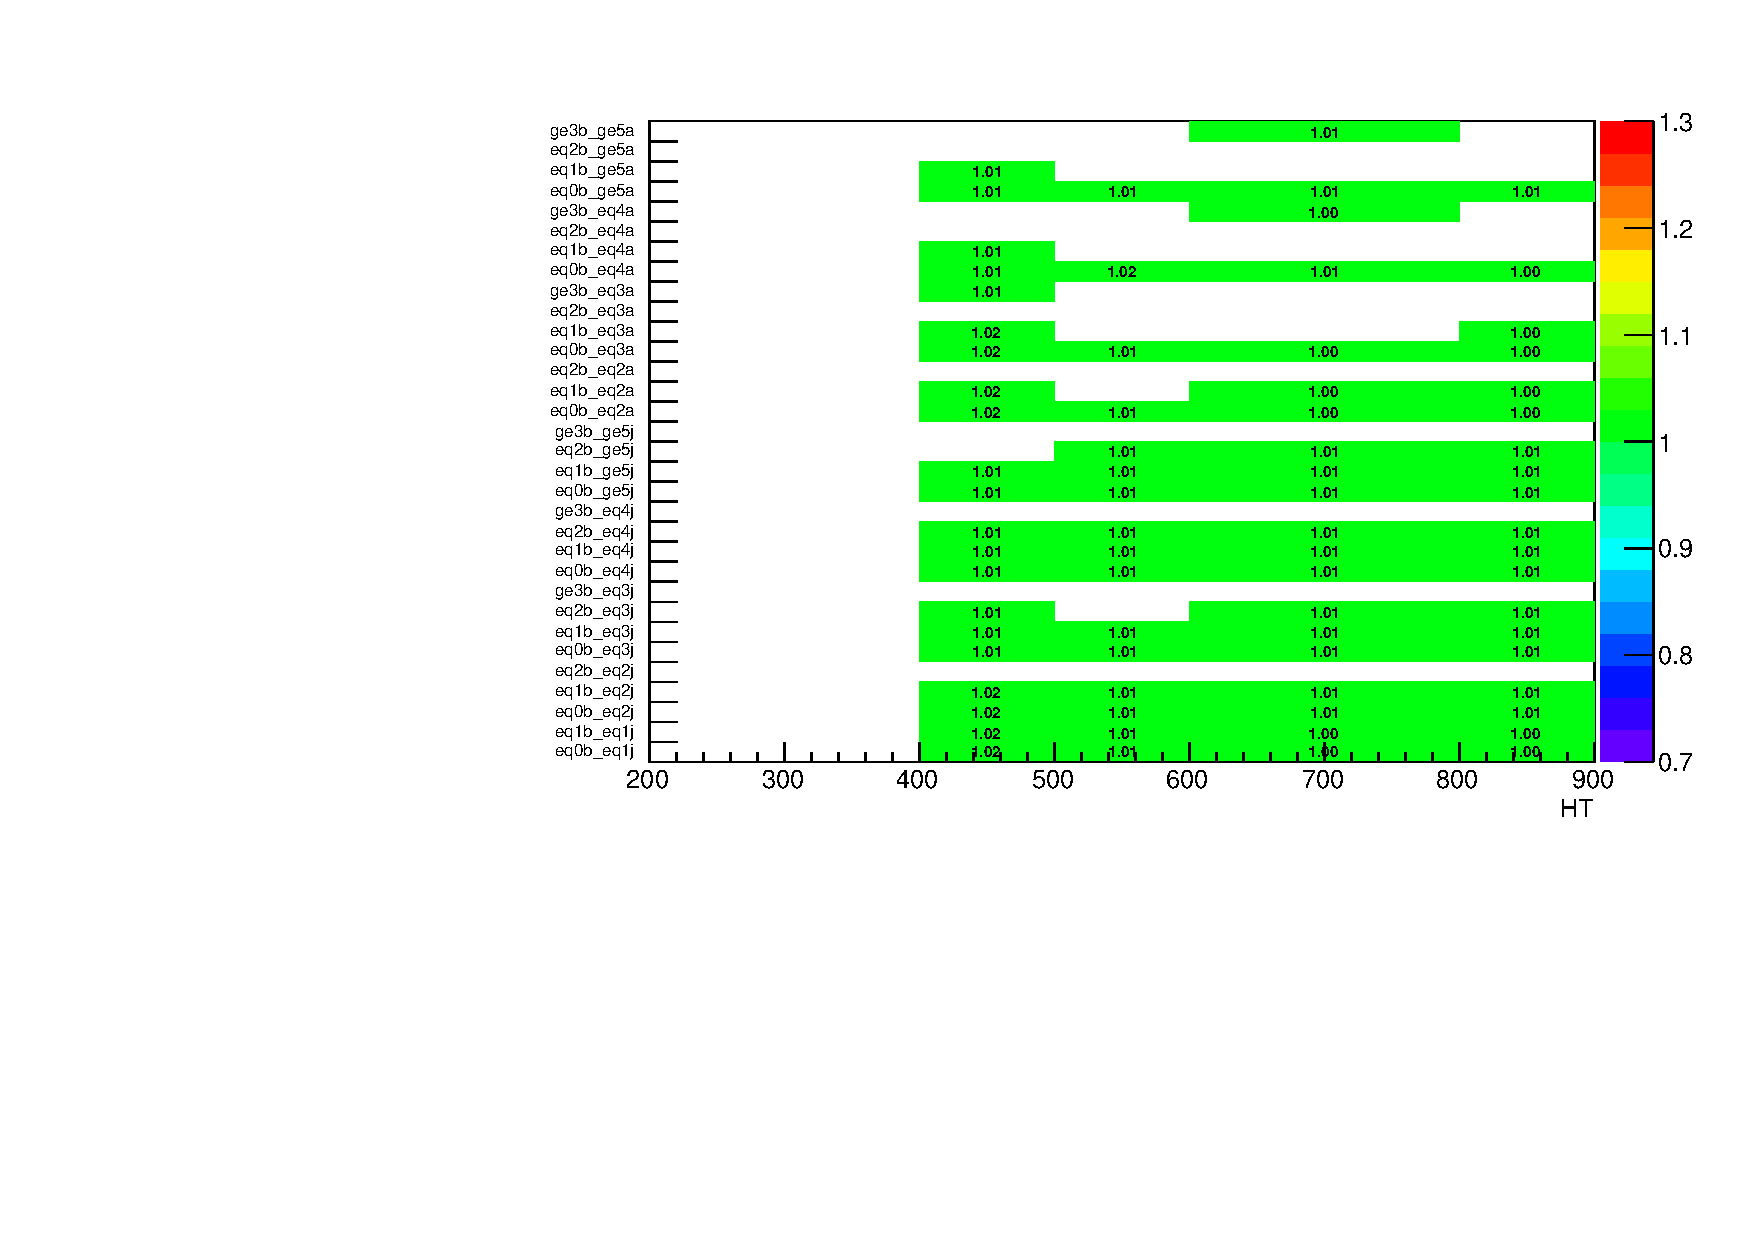
\includegraphics[width=0.4\textwidth]{Figures/backgroundPrediction/mcSystematics12p9fb/Zinv/gj/ratiotfh_ht_mht_allphotonTriggerWeight_Down.pdf}
%  }\\
%
%  \caption{\label{fig:tfSyst_photonTrigger_gjToZinv} The relative change in
%  the $\gj \rightarrow (\znunu)$ transfer
%  factors when varying photon trigger weight in MC within its uncertainties, as a function of \scalht and jet category. 
%  Variations corresponding to $+1\sigma$ ($-1\sigma$) are shown in the left (right) figure. 
%  }
% \end{figure}
%
% \clearpage
% \section{Signal trigger uncertainty}
%
% \begin{figure}[!h]
%   \centering
%   \subfloat[trigger weight up variation]{
%     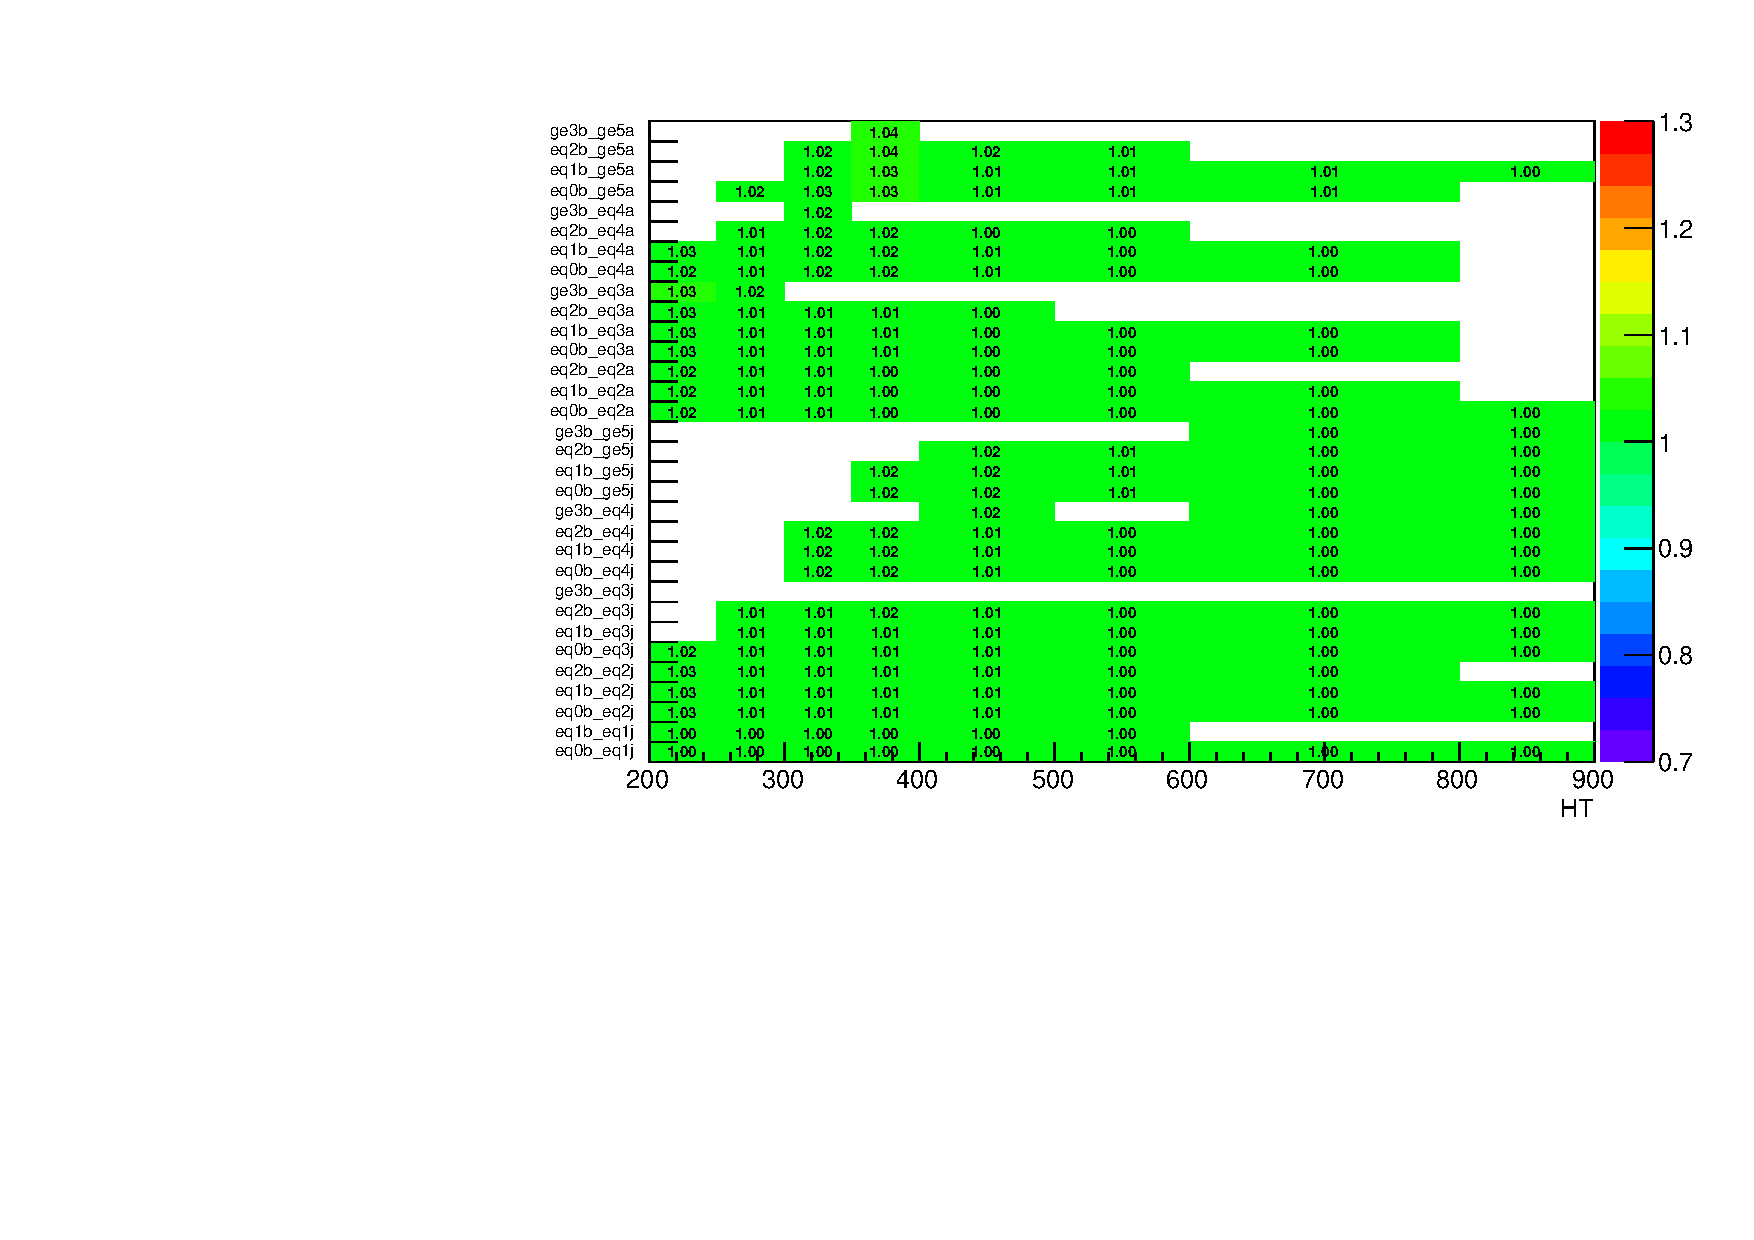
\includegraphics[width=0.4\textwidth]{Figures/backgroundPrediction/mcSystematics12p9fb/Zinv/mu/ratiotfh_ht_mht_alltriggerWeight_Up.pdf}
%   } ~~
%   \subfloat[trigger weight down variation]{
%     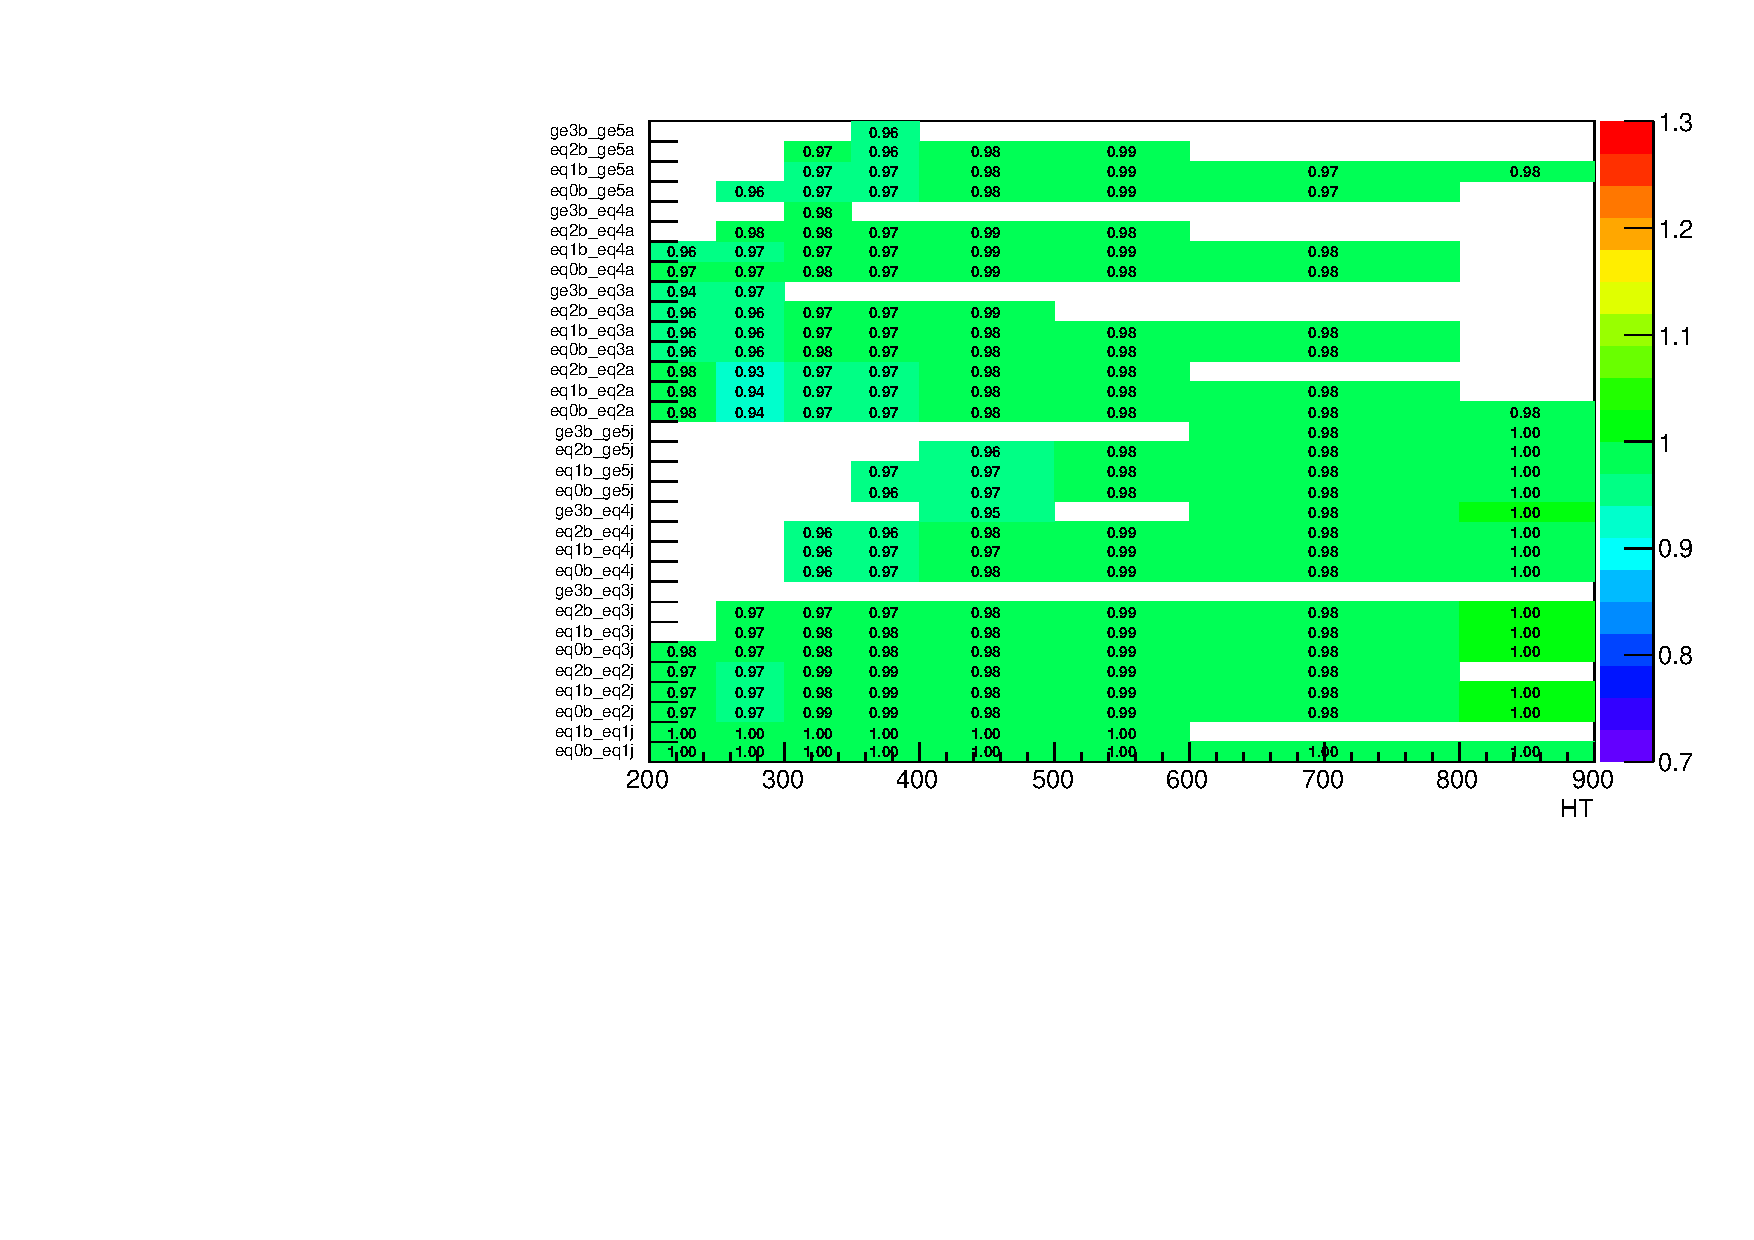
\includegraphics[width=0.4\textwidth]{Figures/backgroundPrediction/mcSystematics12p9fb/Zinv/mu/ratiotfh_ht_mht_alltriggerWeight_Down.pdf}
%   }\\
%
%   \caption{\label{fig:tfSyst_trigger_muToZinv} The relative change in
%   the $\mj \rightarrow (\znunu)$ transfer
%   factors when varying trigger weight in MC within its uncertainties, as a function of \scalht and jet category. 
%   Variations corresponding to $+1\sigma$ ($-1\sigma$) are shown in the left (right) figure. 
%   }
% \end{figure}
% \begin{figure}[!h]
%   \centering
%   \subfloat[trigger weight up variation]{
%     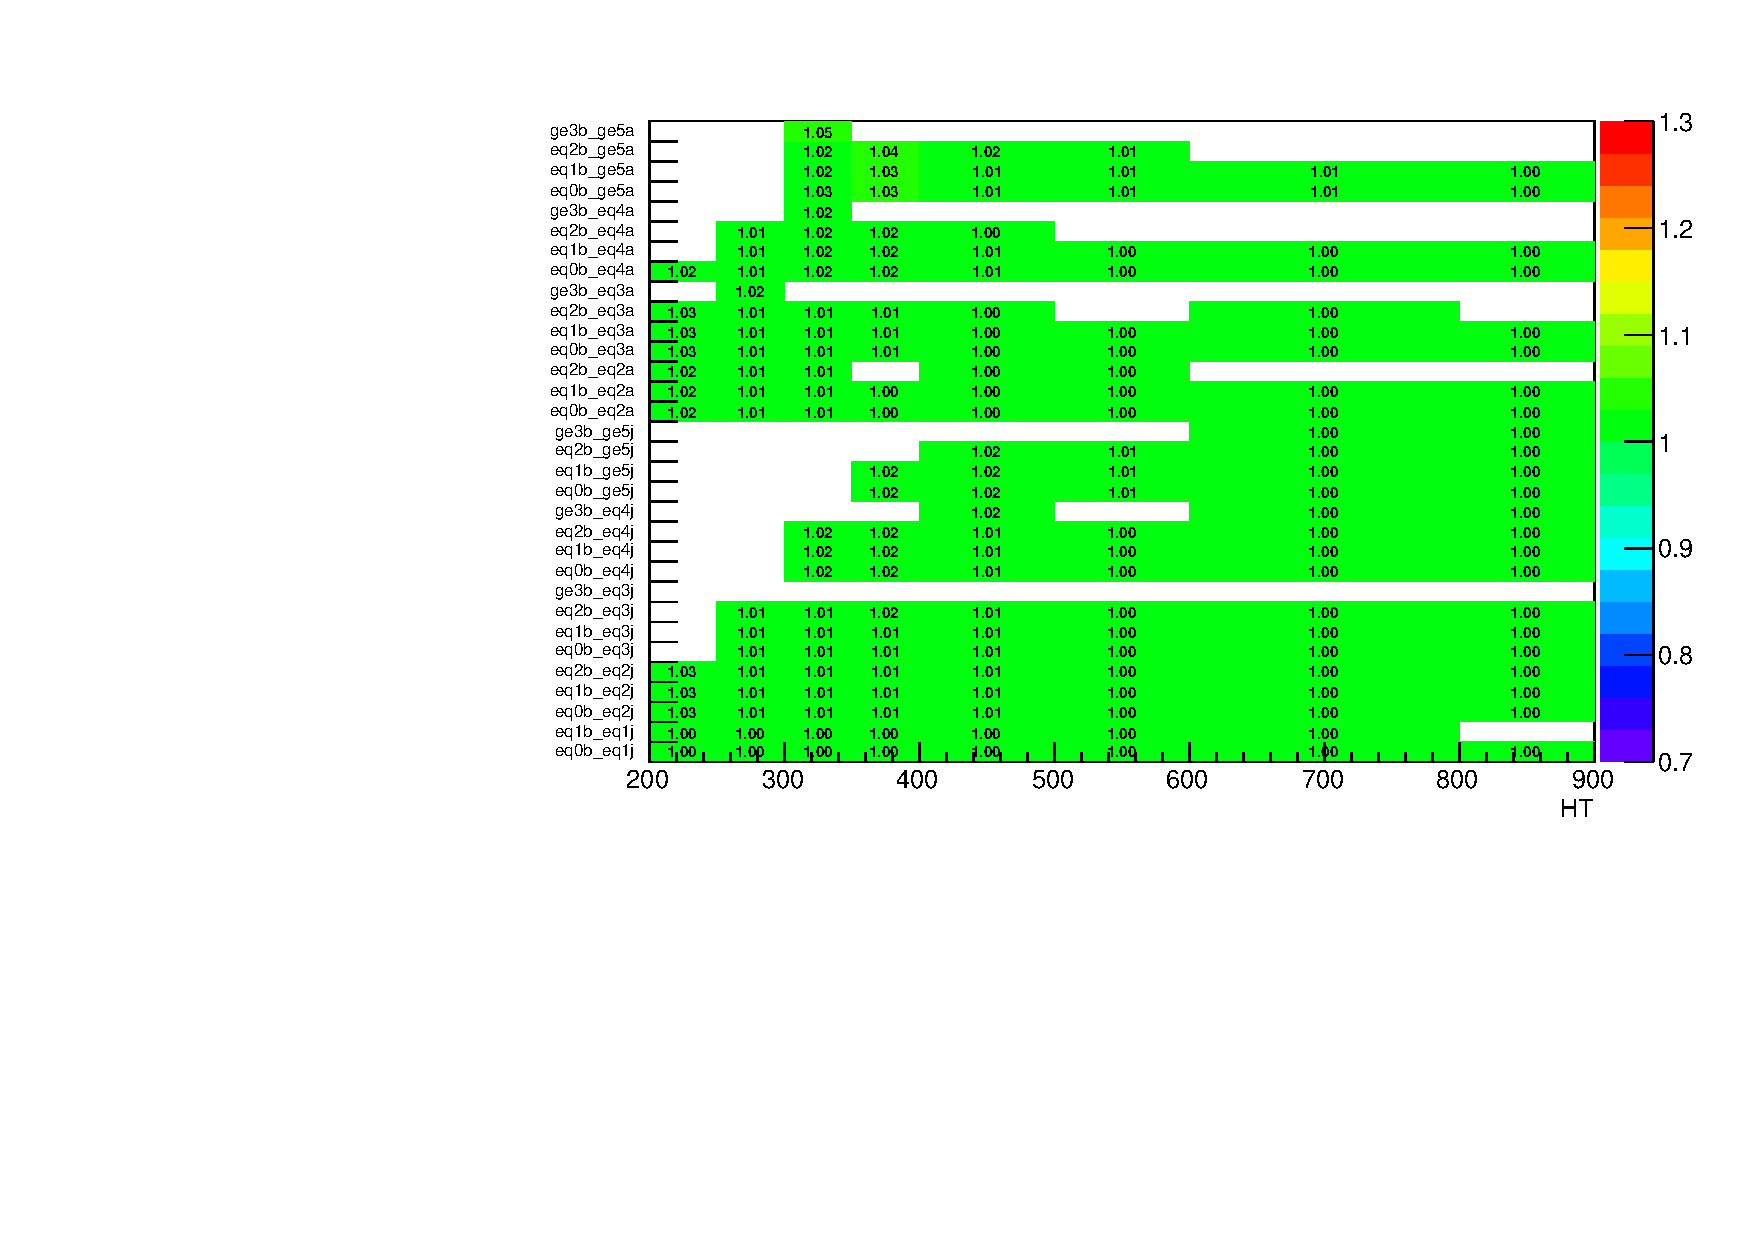
\includegraphics[width=0.4\textwidth]{Figures/backgroundPrediction/mcSystematics12p9fb/Zinv/mumu/ratiotfh_ht_mht_alltriggerWeight_Up.pdf}
%   } ~~
%   \subfloat[trigger weight down variation]{
%     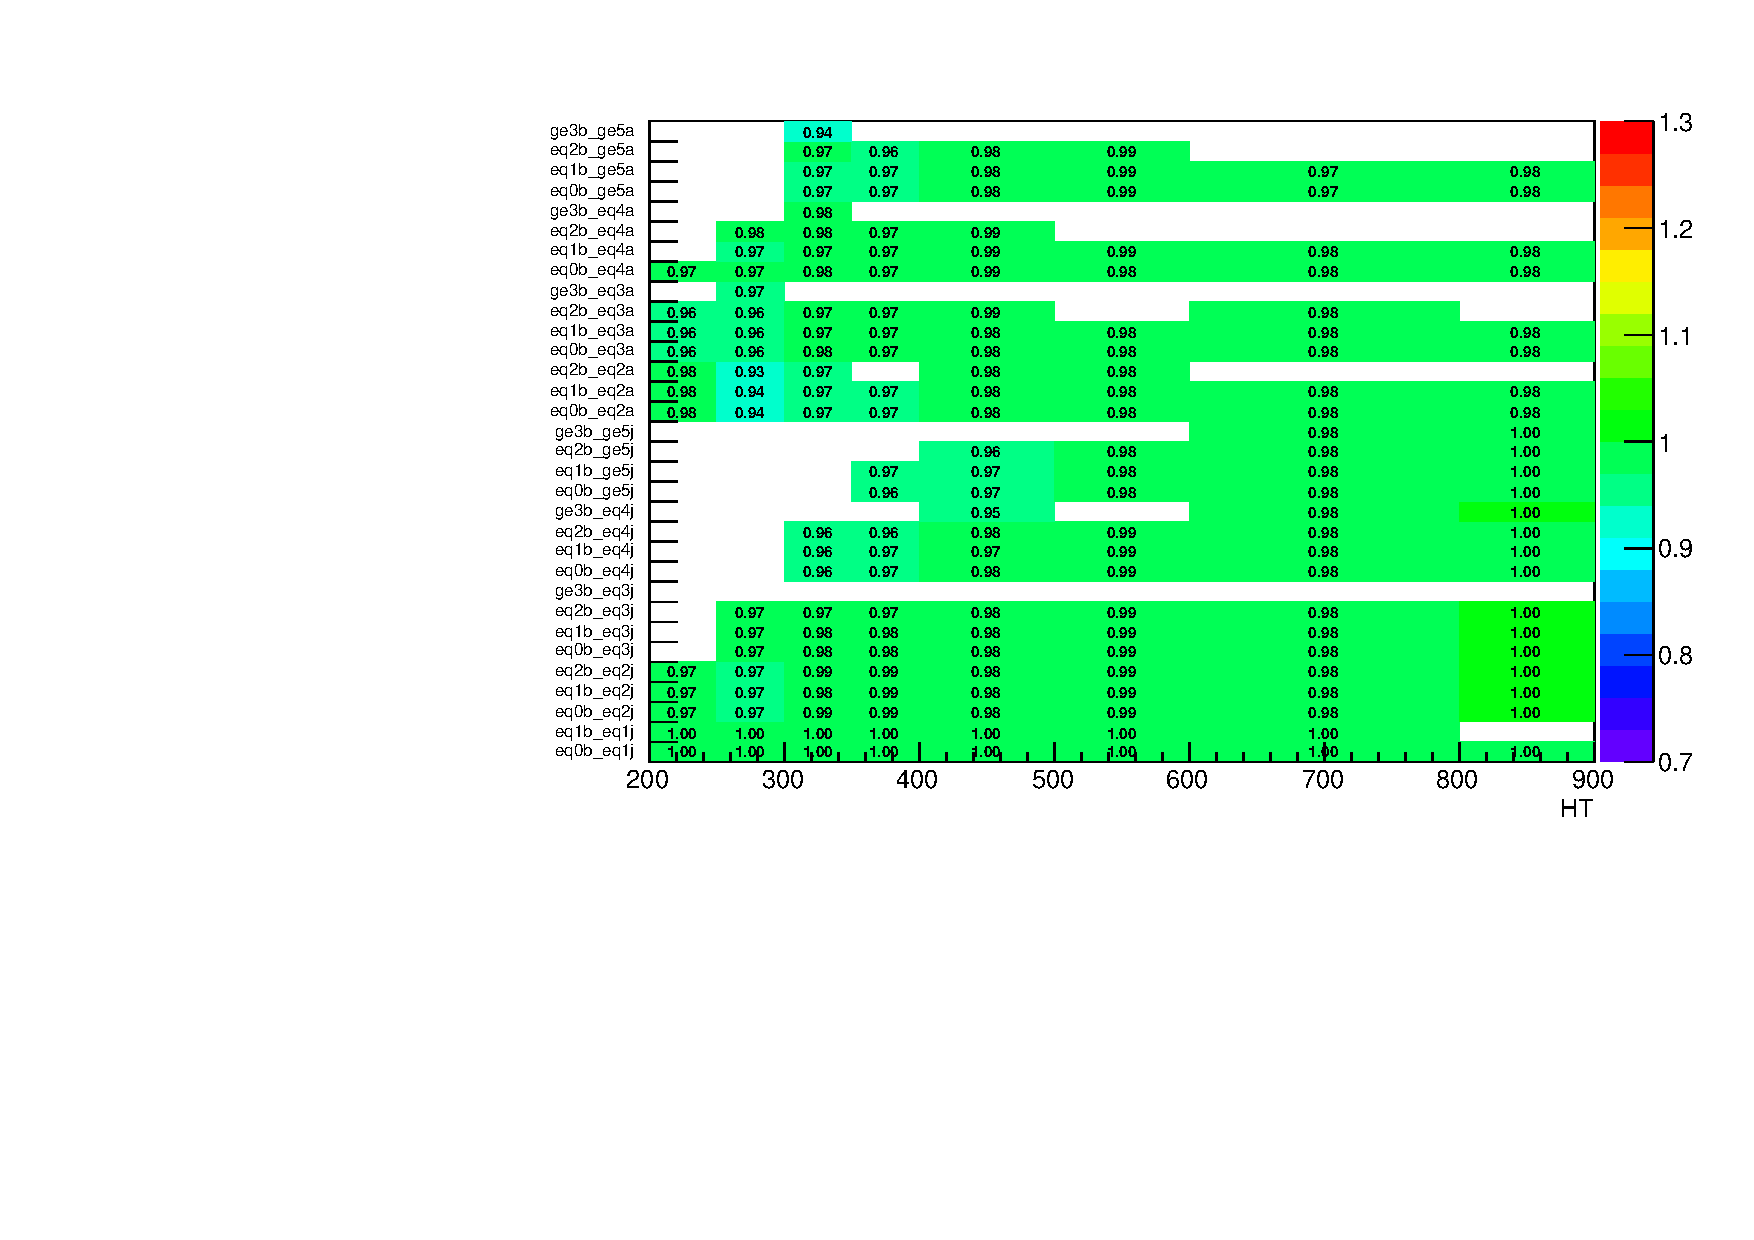
\includegraphics[width=0.4\textwidth]{Figures/backgroundPrediction/mcSystematics12p9fb/Zinv/mumu/ratiotfh_ht_mht_alltriggerWeight_Down.pdf}
%   }\\
%
%   \caption{\label{fig:tfSyst_trigger_mumuToZinv} The relative change in
%   the $\mmj \rightarrow (\znunu)$ transfer
%   factors when varying trigger weight in MC within its uncertainties, as a function of \scalht and jet category. 
%   Variations corresponding to $+1\sigma$ ($-1\sigma$) are shown in the left (right) figure. 
%   }
% \end{figure}
%
% \begin{figure}[!h]
%   \centering
%   \subfloat[trigger weight up variation]{
%     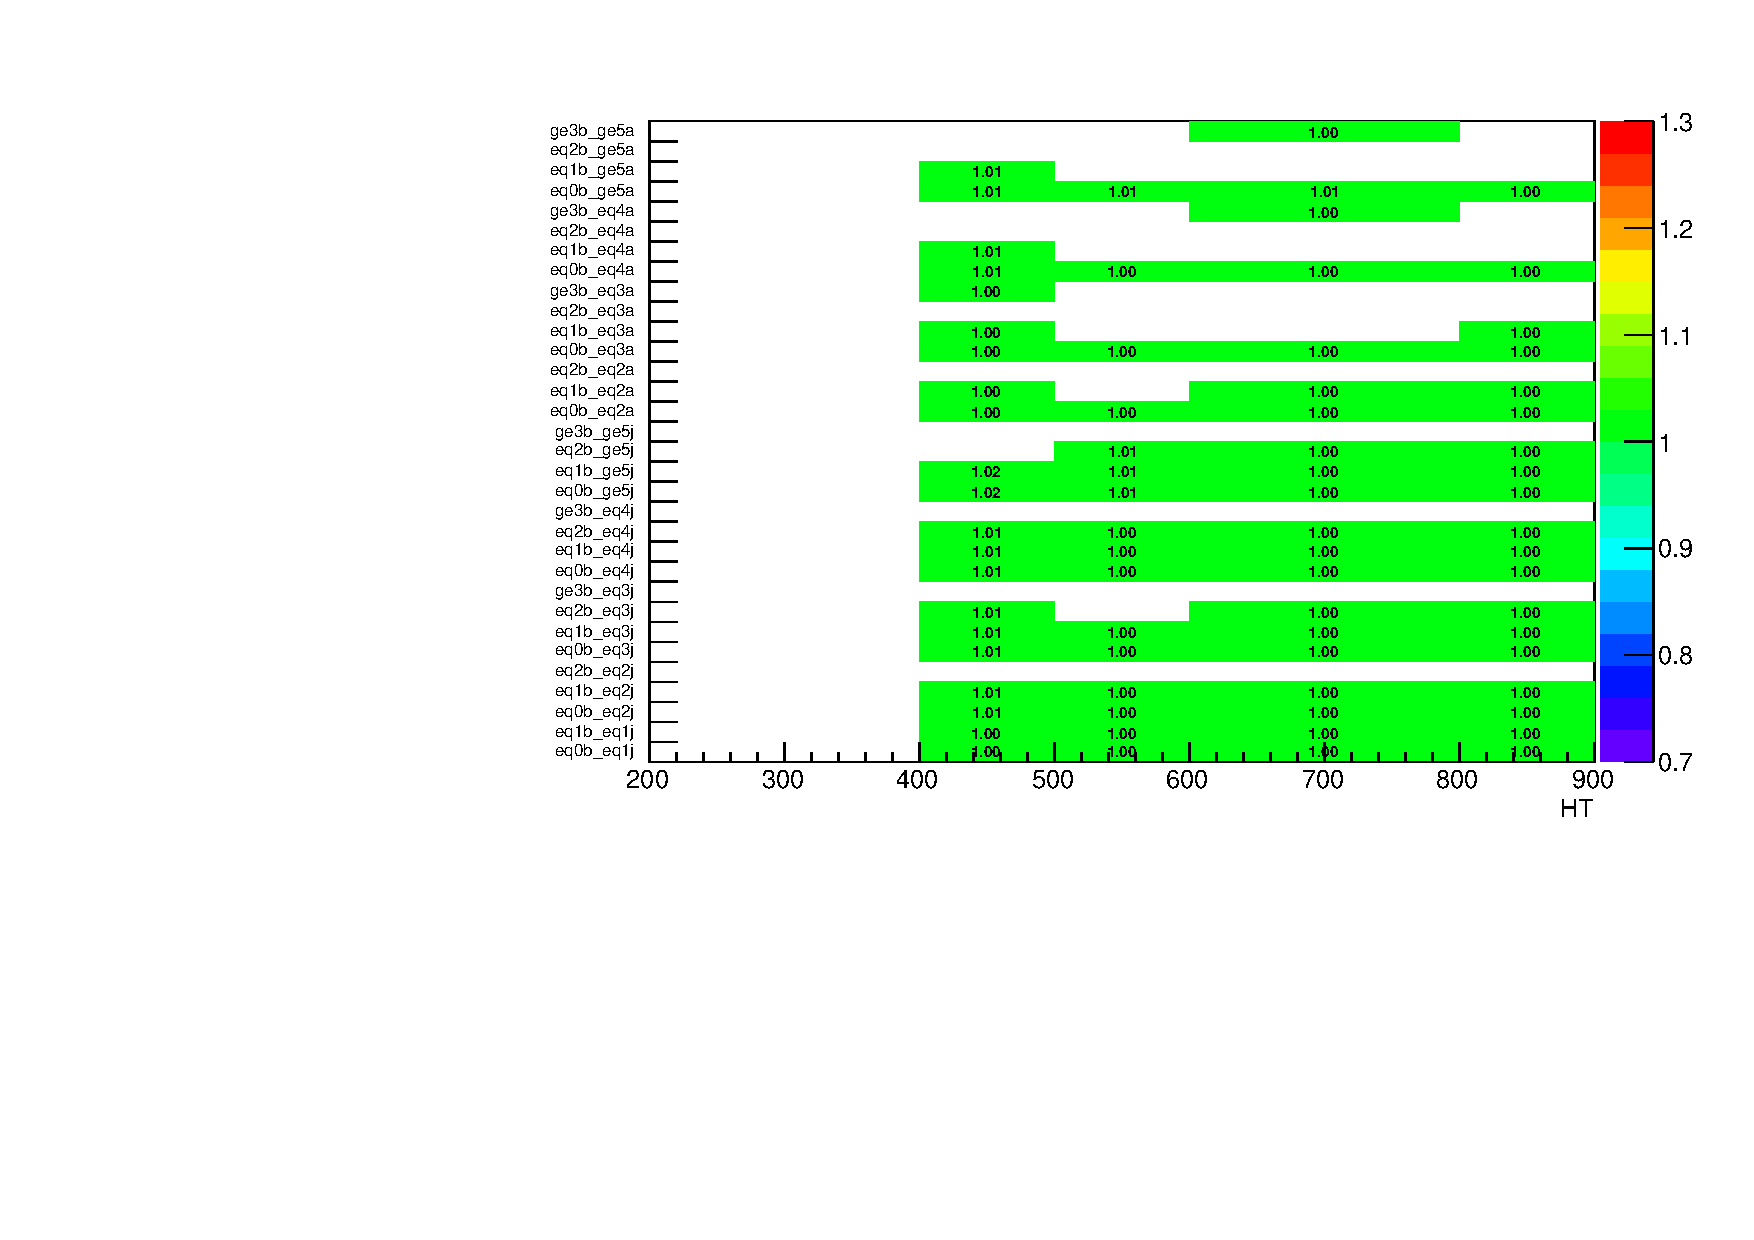
\includegraphics[width=0.4\textwidth]{Figures/backgroundPrediction/mcSystematics12p9fb/Zinv/gj/ratiotfh_ht_mht_alltriggerWeight_Up.pdf}
%   } ~~
%   \subfloat[trigger weight down variation]{
%     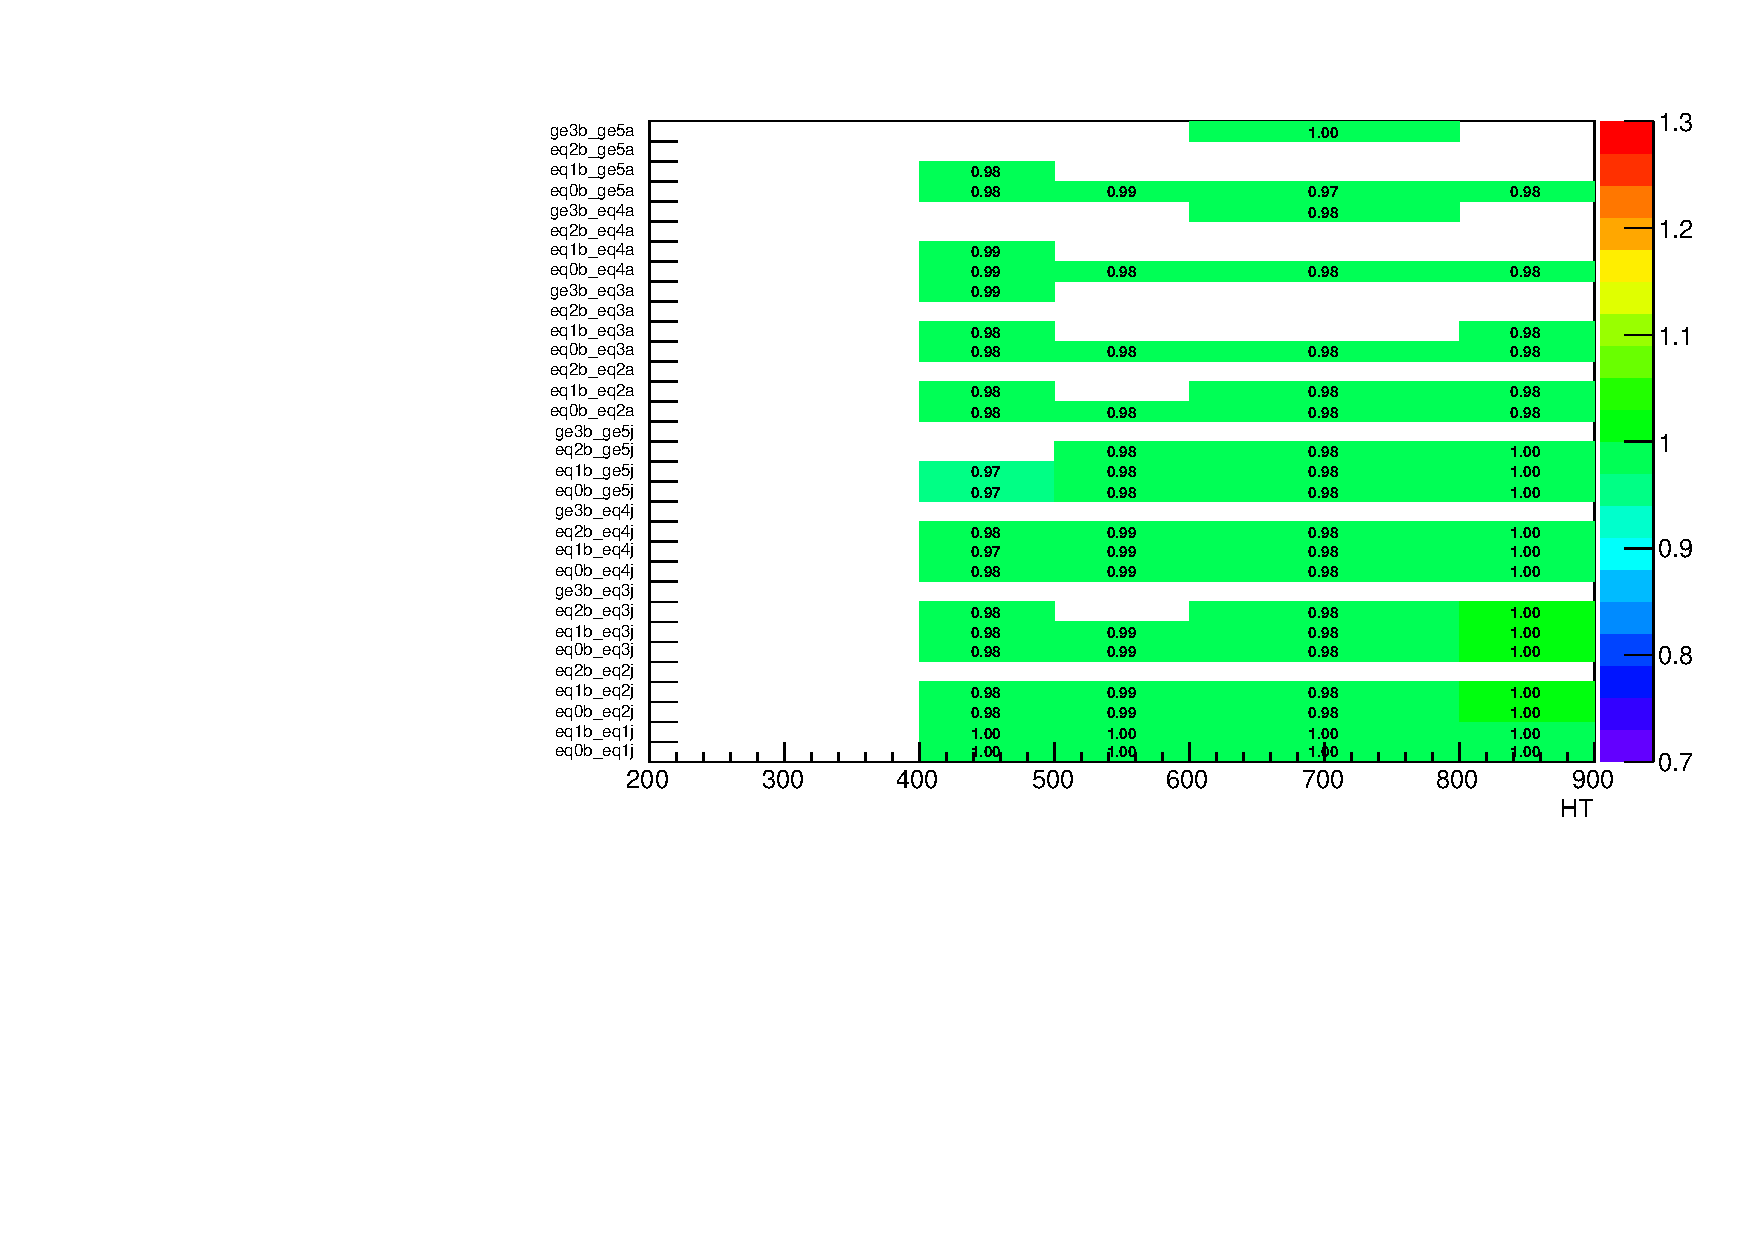
\includegraphics[width=0.4\textwidth]{Figures/backgroundPrediction/mcSystematics12p9fb/Zinv/gj/ratiotfh_ht_mht_alltriggerWeight_Down.pdf}
%   }\\
%
%   \caption{\label{fig:tfSyst_trigger_gjToZinv} The relative change in
%   the $\gj \rightarrow (\znunu)$ transfer
%   factors when varying trigger weight in MC within its uncertainties, as a function of \scalht and jet category. 
%   Variations corresponding to $+1\sigma$ ($-1\sigma$) are shown in the left (right) figure. 
%   }
% \end{figure}
%
% \begin{figure}[!h]
%   \centering
%   \subfloat[trigger weight up variation]{
%     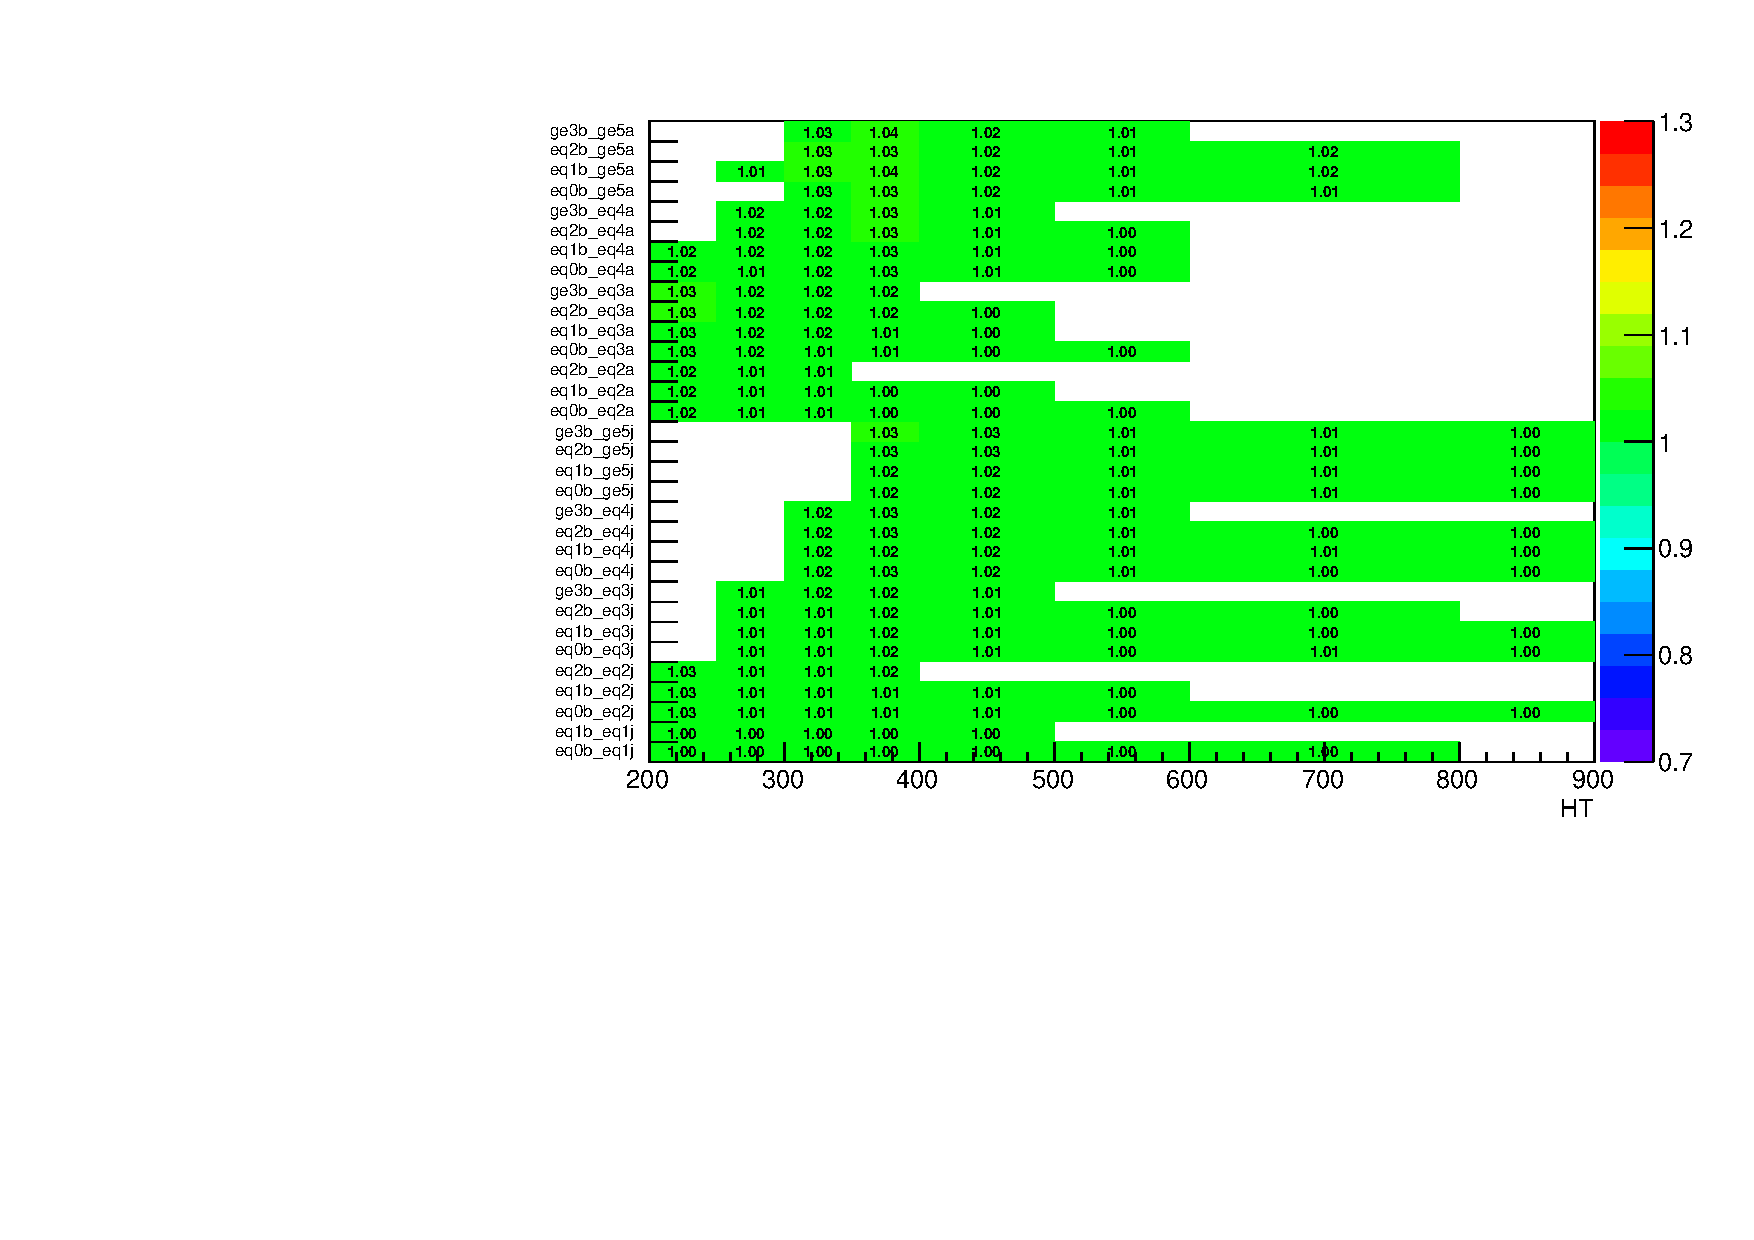
\includegraphics[width=0.4\textwidth]{Figures/backgroundPrediction/mcSystematics12p9fb/Ttw/mu/ratiotfh_ht_mht_alltriggerWeight_Up.pdf}
%   } ~~
%   \subfloat[trigger weight down variation]{
%     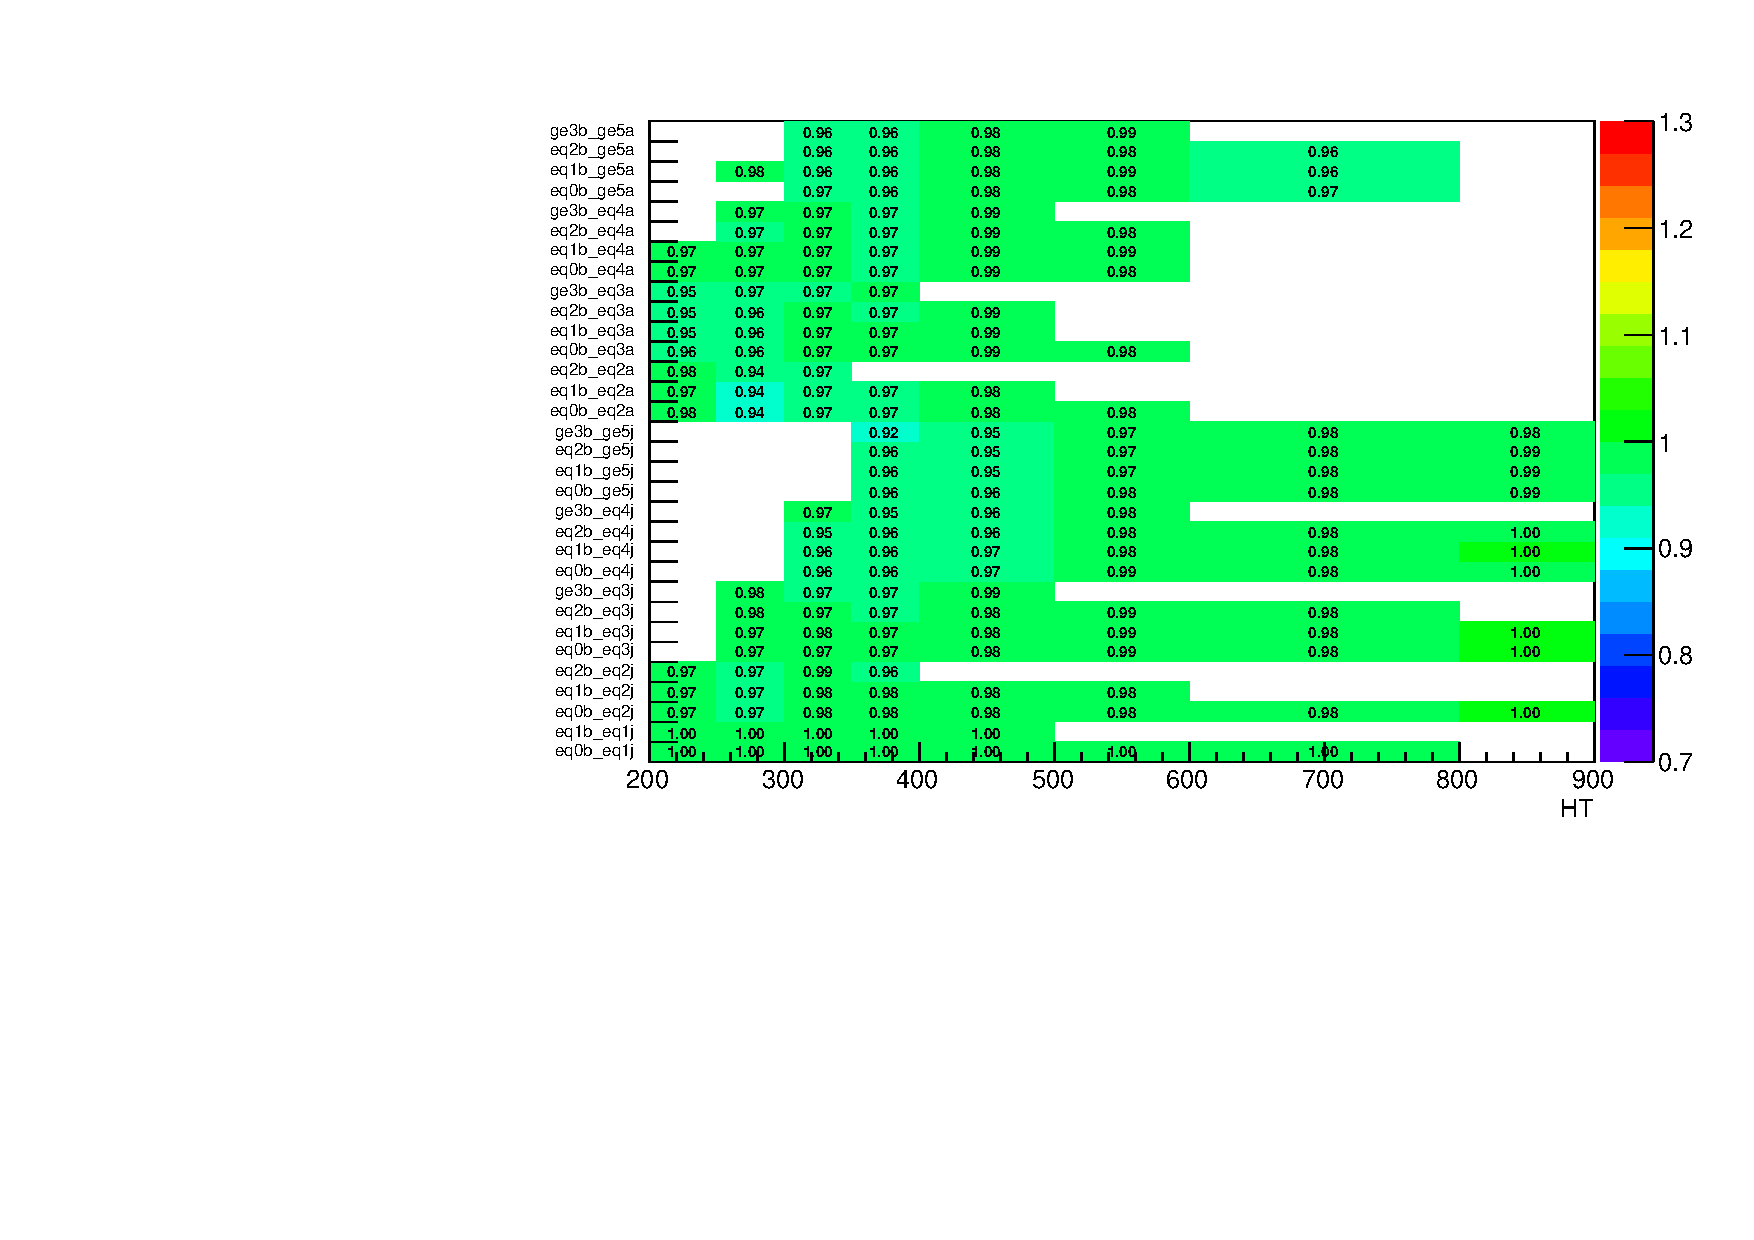
\includegraphics[width=0.4\textwidth]{Figures/backgroundPrediction/mcSystematics12p9fb/Ttw/mu/ratiotfh_ht_mht_alltriggerWeight_Down.pdf}
%   }\\
%
%   \caption{\label{fig:tfSyst_trigger_muToTtw} The relative change in the $\mj \rightarrow \mathrm{tt+W}$ transfer
%   factors when varying trigger weight in MC within its uncertainties, as a function of \scalht and jet category. 
%   Variations corresponding to $+1\sigma$ ($-1\sigma$) are shown in the left (right) figure. 
%   }
% \end{figure}
%
% \section{Top $p_T$ reweighting}
%
% \begin{figure}[!h]
%  \centering
%  \subfloat[top $p_{T}$ weight up variation]{
%    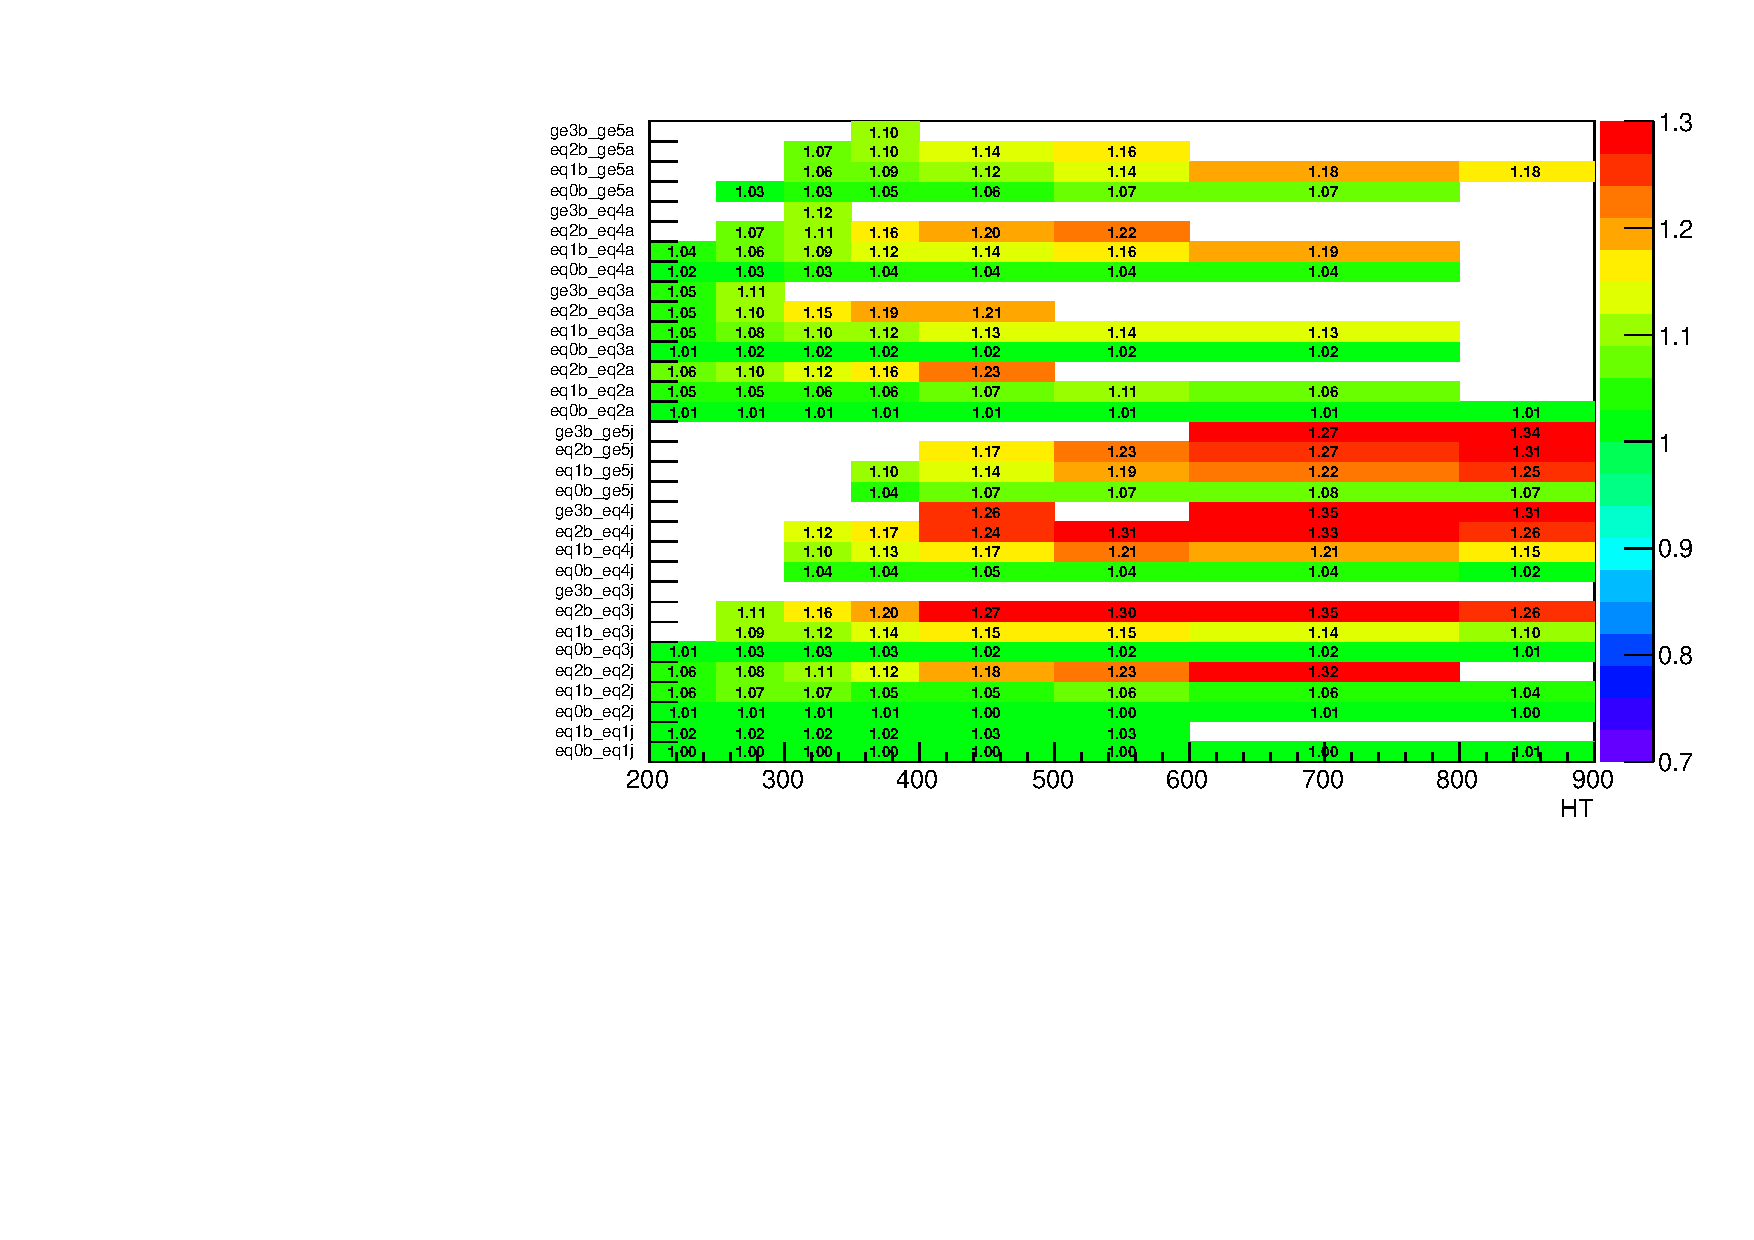
\includegraphics[width=0.4\textwidth]{Figures/backgroundPrediction/mcSystematics12p9fb/Zinv/mu/ratiotfh_ht_mht_alltopPtWeight_Up.pdf}
%  } ~~
%  \subfloat[top $p_{T}$ weight down variation]{
%    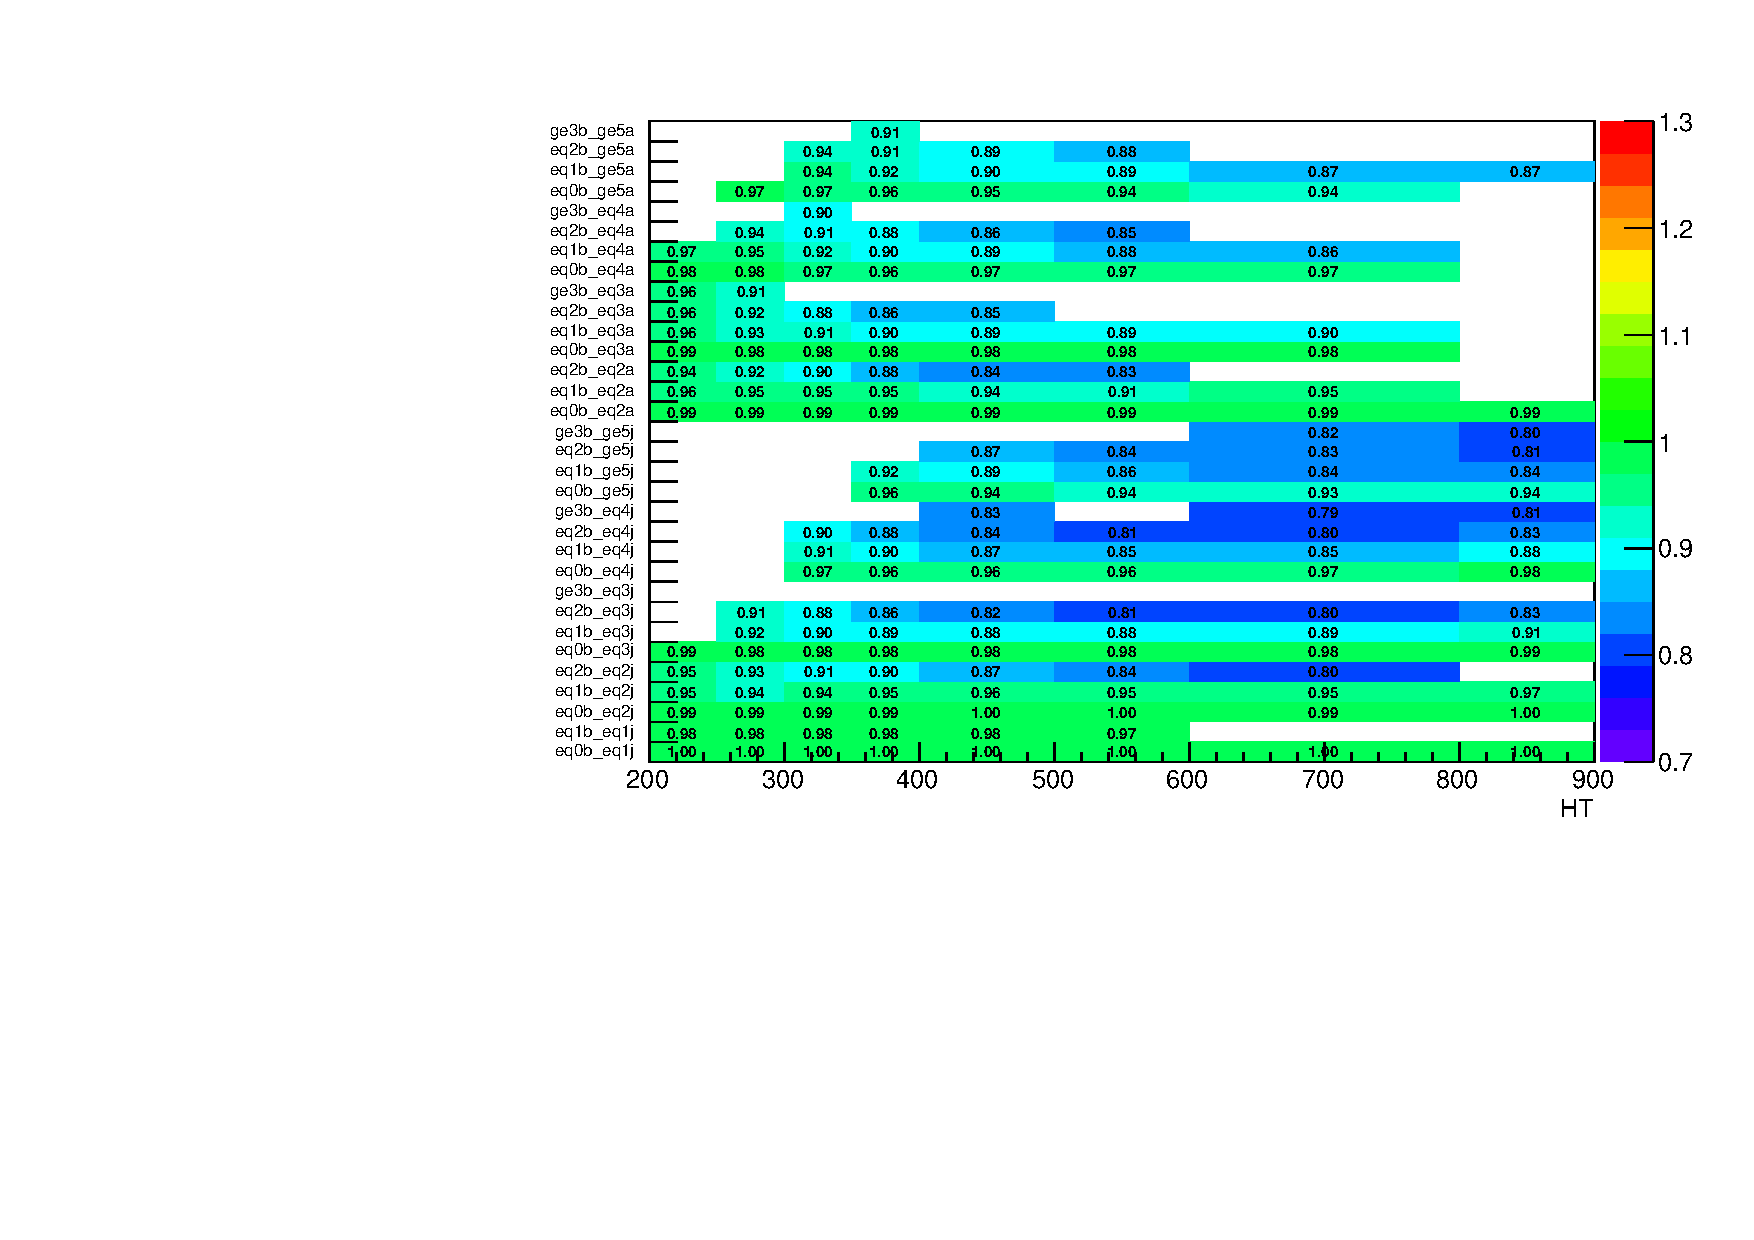
\includegraphics[width=0.4\textwidth]{Figures/backgroundPrediction/mcSystematics12p9fb/Zinv/mu/ratiotfh_ht_mht_alltopPtWeight_Down.pdf}
%  }\\
%
%  \caption{\label{fig:tfSyst_topPt_muToZinv} The relative change in
%  the $\mj \rightarrow (\znunu)$ transfer
%  factors when varying top $p_{T}$ weight in MC within its uncertainties, as a function of \scalht and jet category. 
%  Variations corresponding to $+1\sigma$ ($-1\sigma$) are shown in the left (right) figure. 
%  }
% \end{figure}
%
% \begin{figure}[!h]
%  \centering
%  \subfloat[top $p_{T}$ weight up variation]{
%    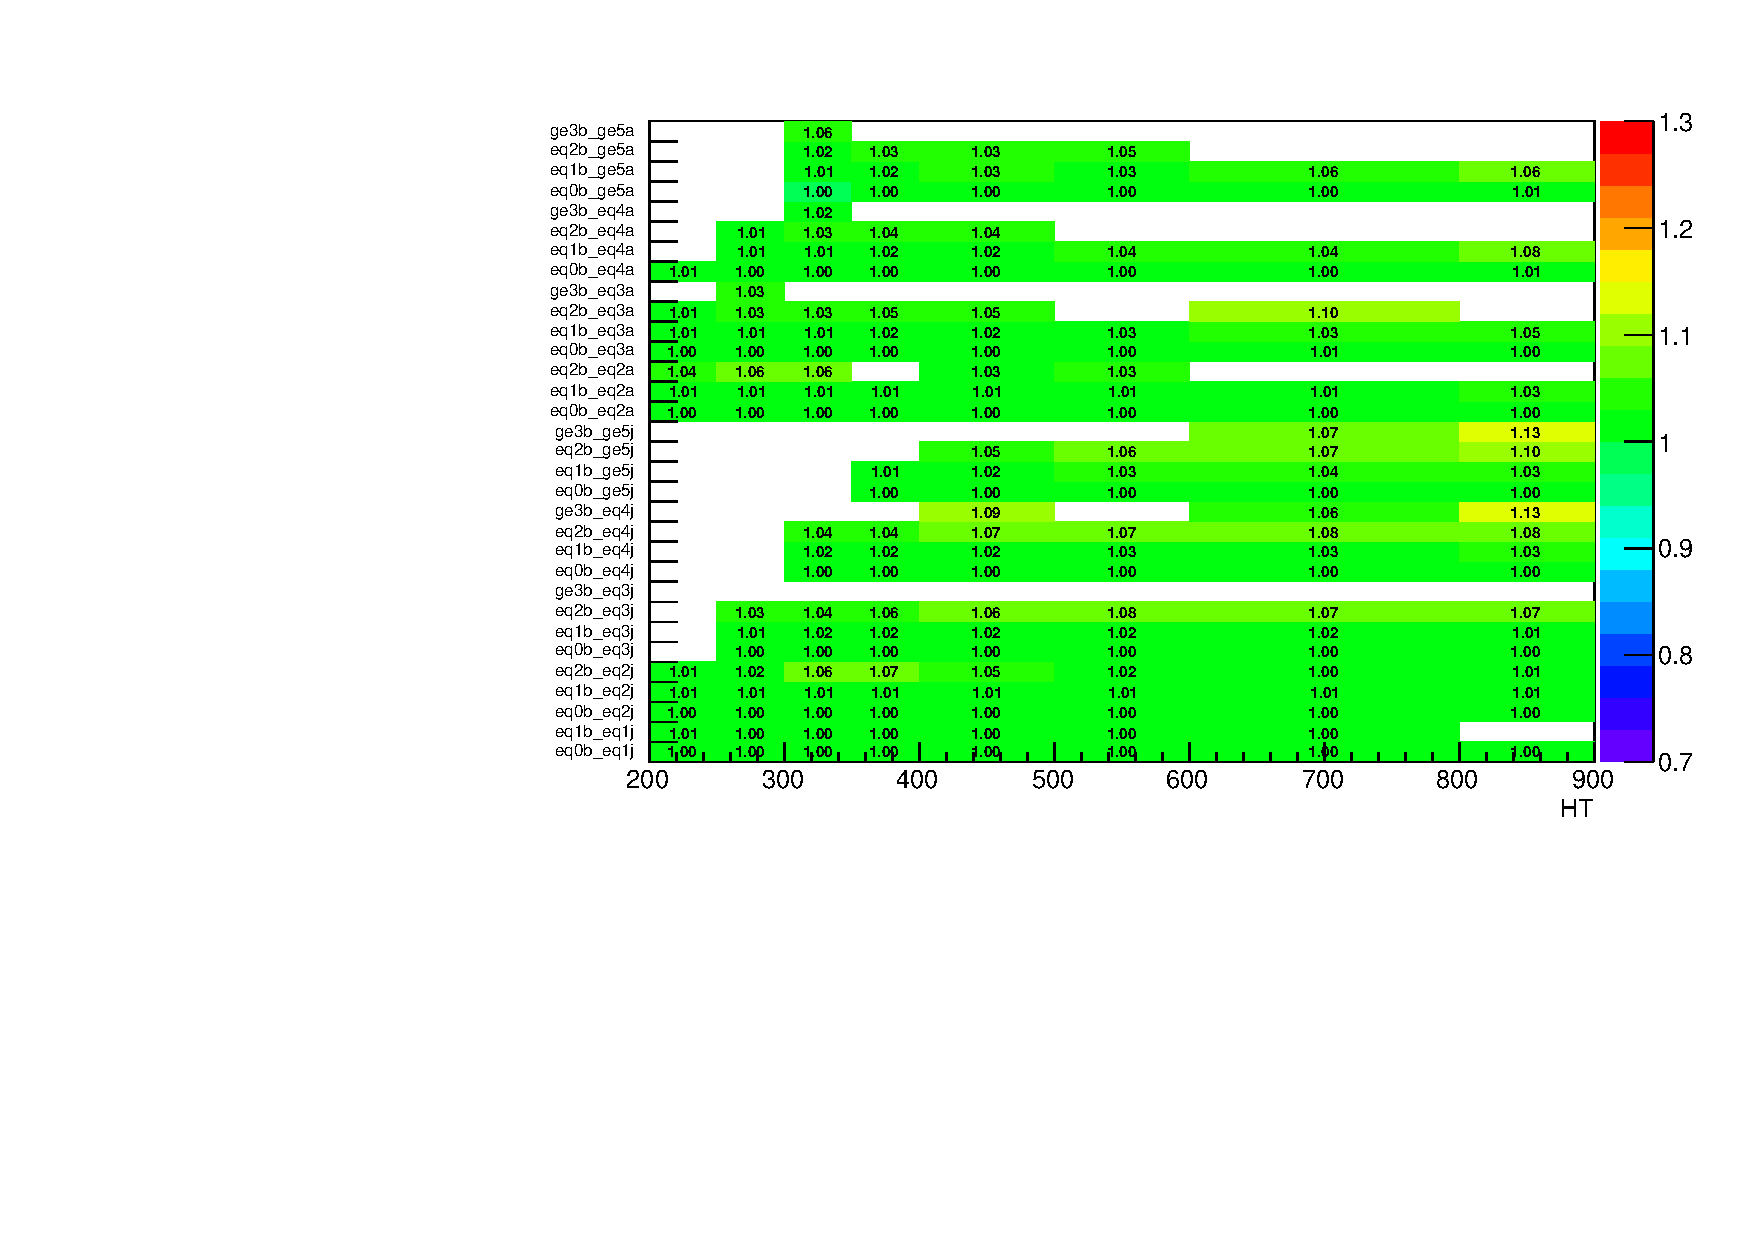
\includegraphics[width=0.4\textwidth]{Figures/backgroundPrediction/mcSystematics12p9fb/Zinv/mumu/ratiotfh_ht_mht_alltopPtWeight_Up.pdf}
%  } ~~
%  \subfloat[top $p_{T}$ weight down variation]{
%    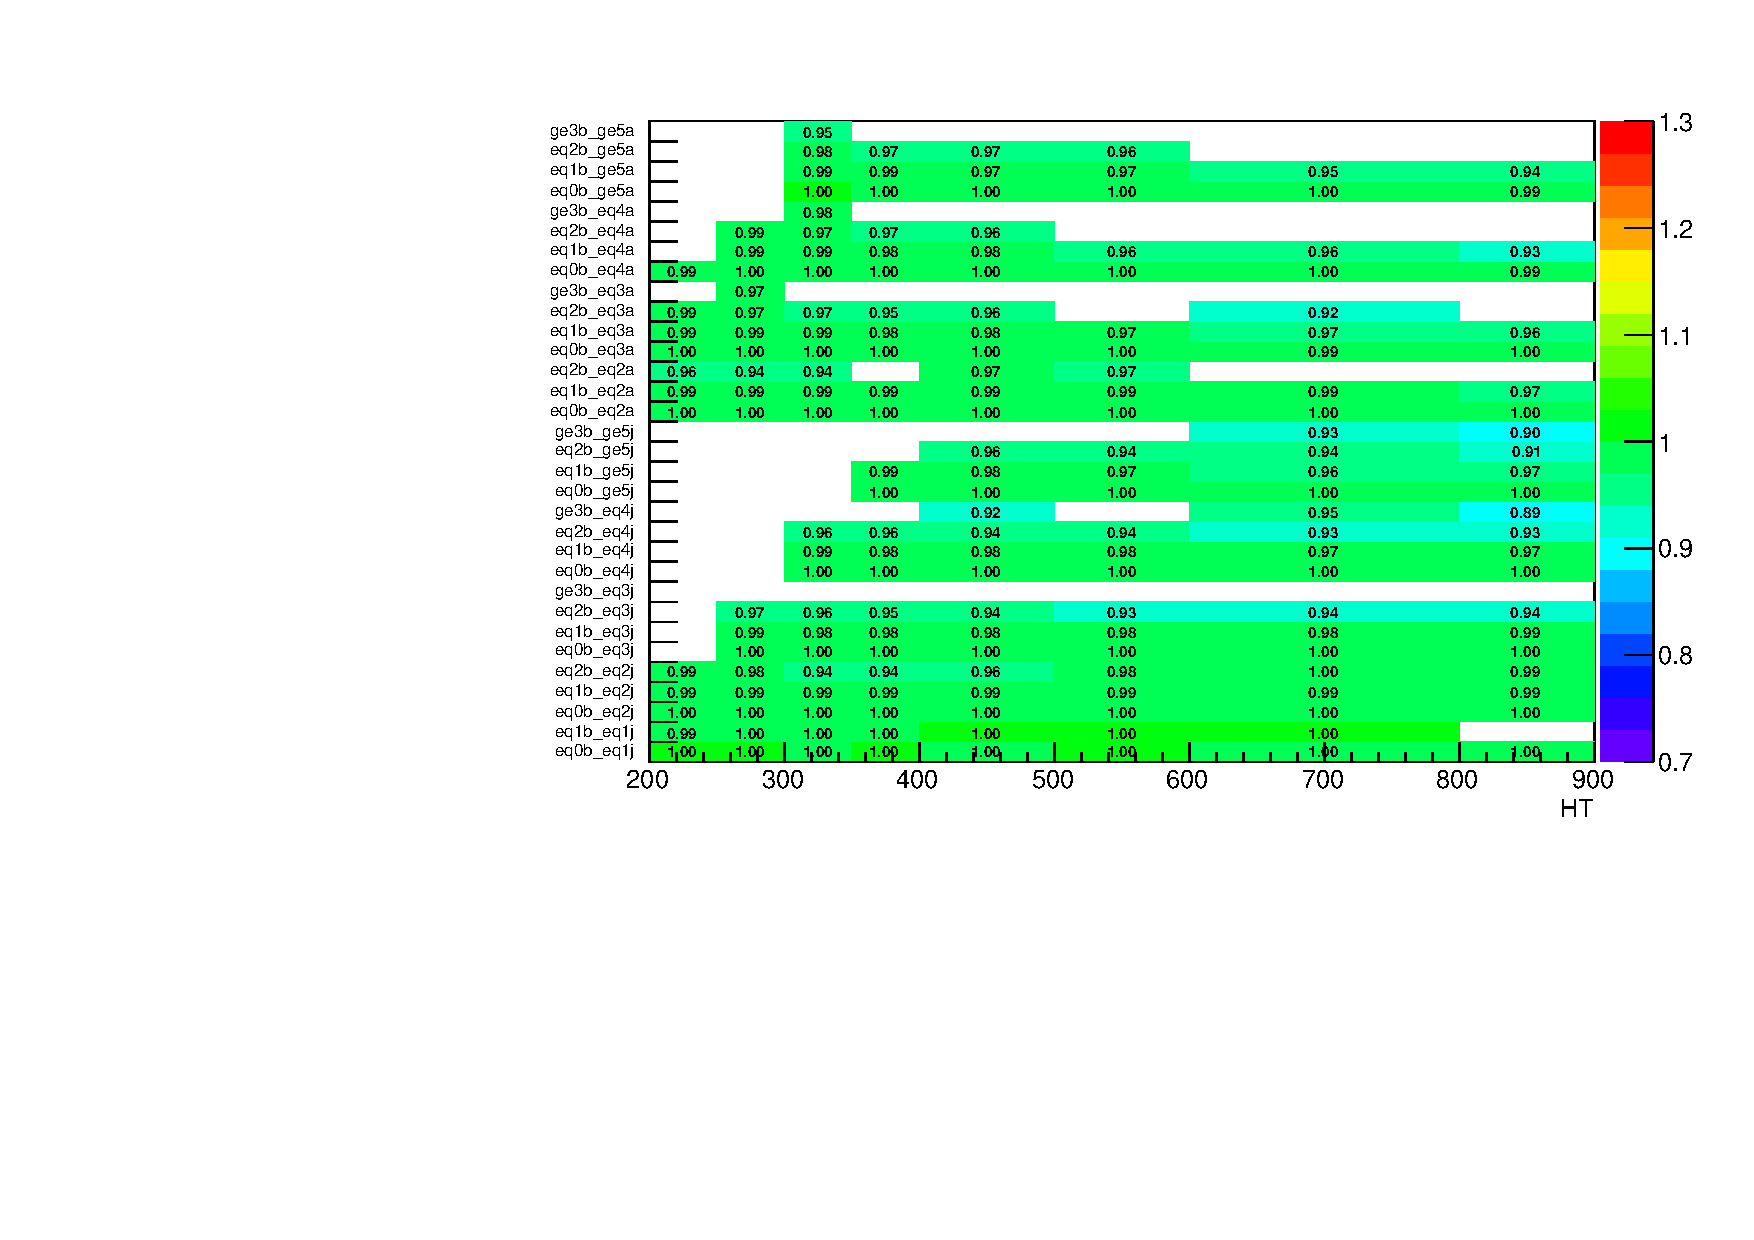
\includegraphics[width=0.4\textwidth]{Figures/backgroundPrediction/mcSystematics12p9fb/Zinv/mumu/ratiotfh_ht_mht_alltopPtWeight_Down.pdf}
%  }\\
%
%  \caption{\label{fig:tfSyst_topPt_mumuToZinv} The relative change in
%  the $\mmj \rightarrow (\znunu)$ transfer
%  factors when varying top $p_{T}$ weight in MC within its uncertainties, as a function of \scalht and jet category. 
%  Variations corresponding to $+1\sigma$ ($-1\sigma$) are shown in the left (right) figure. 
%  }
% \end{figure}
%
% \begin{figure}[!h]
%  \centering
%  \subfloat[top $p_{T}$ weight up variation]{
%    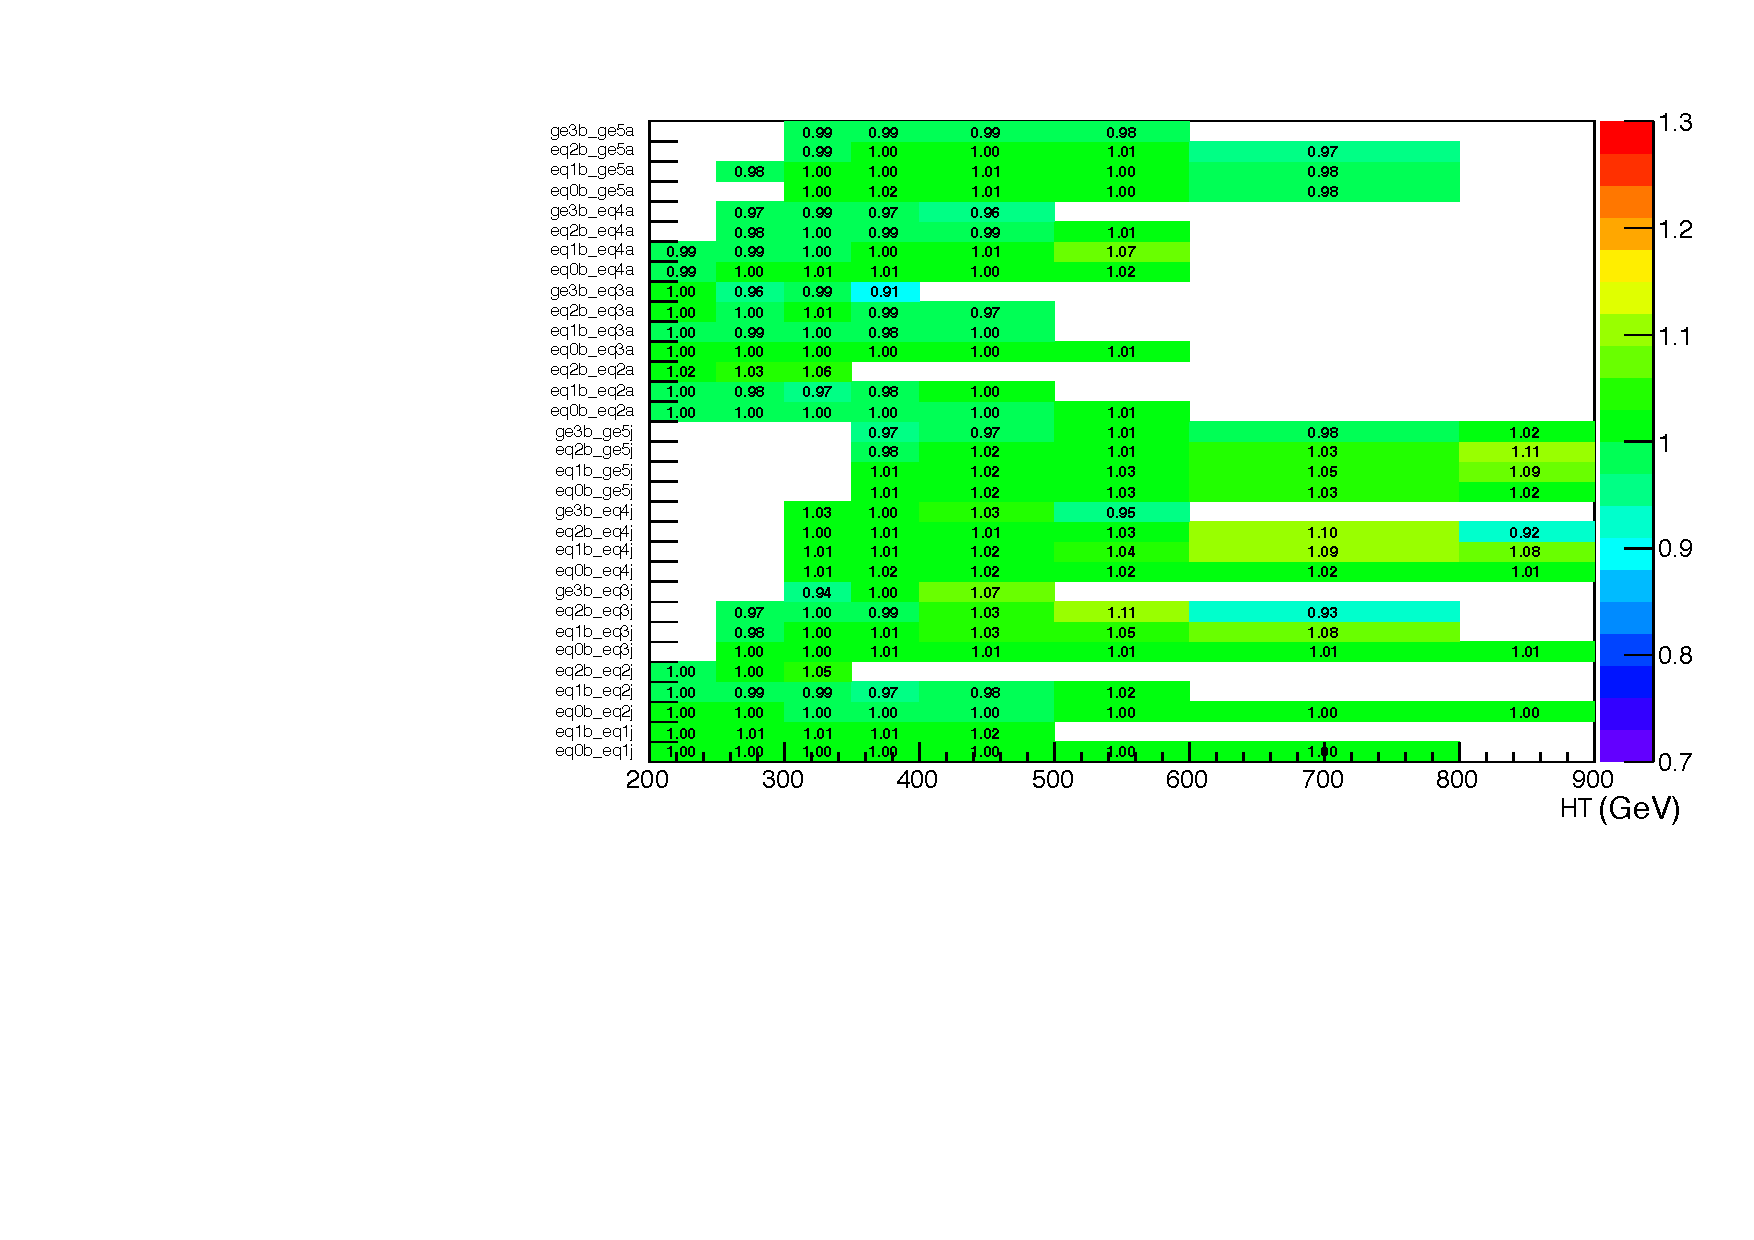
\includegraphics[width=0.4\textwidth]{Figures/backgroundPrediction/mcSystematics12p9fb/Ttw/mu/ratiotfh_ht_mht_alltopPtWeight_Up.pdf}
%  } ~~
%  \subfloat[top $p_{T}$ weight down variation]{
%    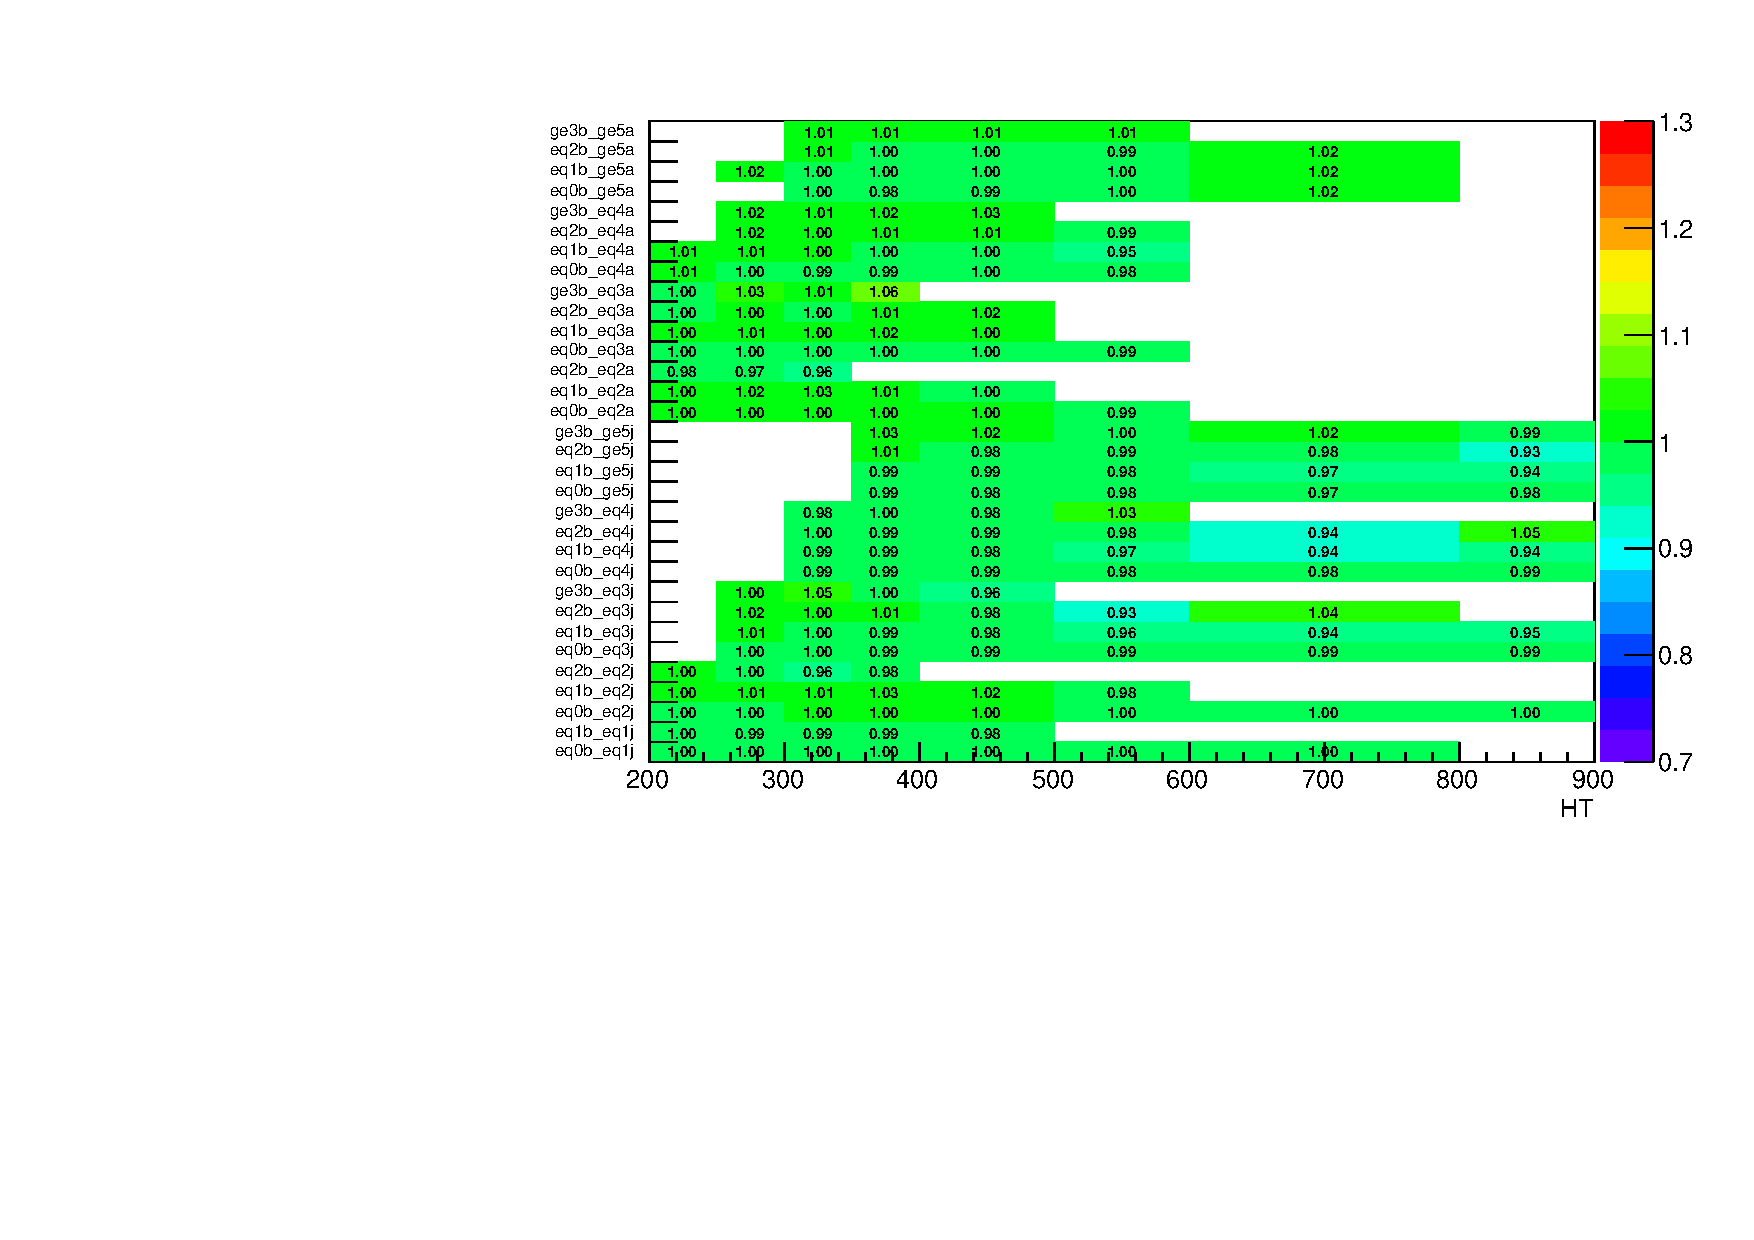
\includegraphics[width=0.4\textwidth]{Figures/backgroundPrediction/mcSystematics12p9fb/Ttw/mu/ratiotfh_ht_mht_alltopPtWeight_Down.pdf}
%  }\\
%
%  \caption{\label{fig:tfSyst_topPt_muToTtw} The relative change in the $\mj \rightarrow \mathrm{tt+W}$ transfer
%  factors when varying top $p_{T}$ weight in MC within its uncertainties, as a function of \scalht and jet category. 
%  Variations corresponding to $+1\sigma$ ($-1\sigma$) are shown in the left (right) figure. 
%  }
% \end{figure}
%
% \clearpage
% \section{PU reweighting}
%
% \begin{figure}[!h]
%   \centering
%   \subfloat[PU weight up variation]{
%     \includegraphics[width=0.4\textwidth]{Figures/backgroundPrediction/mcSystematics12p9fb/Zinv/mu/ratiotfh_ht_mht_allpuWeight_Up.pdf}
%   } ~~
%   \subfloat[PU weight down variation]{
%     \includegraphics[width=0.4\textwidth]{Figures/backgroundPrediction/mcSystematics12p9fb/Zinv/mu/ratiotfh_ht_mht_allpuWeight_Down.pdf}
%   }\\
%
%   \caption{\label{fig:tfSyst_pu_muToZinv} The relative change in the
%   $\mj \rightarrow (\znunu)$ transfer
%   factors when varying PU weight in MC within its uncertainties, as a function of \scalht and jet category. 
%   Variations corresponding to $+1\sigma$ ($-1\sigma$) are shown in the left (right) figure. 
%   }
% \end{figure}
%
% \begin{figure}[!h]
%   \centering
%   \subfloat[PU weight up variation]{
%     \includegraphics[width=0.4\textwidth]{Figures/backgroundPrediction/mcSystematics12p9fb/Zinv/mumu/ratiotfh_ht_mht_allpuWeight_Up.pdf}
%   } ~~
%   \subfloat[PU weight down variation]{
%     \includegraphics[width=0.4\textwidth]{Figures/backgroundPrediction/mcSystematics12p9fb/Zinv/mumu/ratiotfh_ht_mht_allpuWeight_Down.pdf}
%   }\\
%
%   \caption{\label{fig:tfSyst_pu_mumuToZinv} The relative change in the
%   $\mmj \rightarrow (\znunu)$ transfer
%   factors when varying PU weight in MC within its uncertainties, as a function of \scalht and jet category. 
%   Variations corresponding to $+1\sigma$ ($-1\sigma$) are shown in the left (right) figure. 
%   }
% \end{figure}
%
% \begin{figure}[!h]
%   \centering
%   \subfloat[PU weight up variation]{
%     \includegraphics[width=0.4\textwidth]{Figures/backgroundPrediction/mcSystematics12p9fb/Zinv/gj/ratiotfh_ht_mht_allpuWeight_Up.pdf}
%   } ~~
%   \subfloat[PU weight down variation]{
%     \includegraphics[width=0.4\textwidth]{Figures/backgroundPrediction/mcSystematics12p9fb/Zinv/gj/ratiotfh_ht_mht_allpuWeight_Down.pdf}
%   }\\
%
%   \caption{\label{fig:tfSyst_pu_gjToZinv} The relative change in the
%   $\gj \rightarrow (\znunu)$ transfer
%   factors when varying PU weight in MC within its uncertainties, as a function of \scalht and jet category. 
%   Variations corresponding to $+1\sigma$ ($-1\sigma$) are shown in the left (right) figure. 
%   }
% \end{figure}
%
% \begin{figure}[!h]
%   \centering
%   \subfloat[PU weight up variation]{
%     \includegraphics[width=0.4\textwidth]{Figures/backgroundPrediction/mcSystematics12p9fb/Ttw/mu/ratiotfh_ht_mht_allpuWeight_Up.pdf}
%   } ~~
%   \subfloat[PU weight down variation]{
%     \includegraphics[width=0.4\textwidth]{Figures/backgroundPrediction/mcSystematics12p9fb/Ttw/mu/ratiotfh_ht_mht_allpuWeight_Down.pdf}
%   }\\
%
%   \caption{\label{fig:tfSyst_pu_muToTtw} The relative change in the $\mj \rightarrow \mathrm{tt+W}$ transfer
%   factors when varying PU weight in MC within its uncertainties, as a function of \scalht and jet category. 
%   Variations corresponding to $+1\sigma$ ($-1\sigma$) are shown in the left (right) figure. 
%   }
% \end{figure}
